\documentclass[twoside]{book}

% Packages required by doxygen
\usepackage{fixltx2e}
\usepackage{calc}
\usepackage{doxygen}
\usepackage[export]{adjustbox} % also loads graphicx
\usepackage{graphicx}
\usepackage[utf8]{inputenc}
\usepackage{makeidx}
\usepackage{multicol}
\usepackage{multirow}
\PassOptionsToPackage{warn}{textcomp}
\usepackage{textcomp}
\usepackage[nointegrals]{wasysym}
\usepackage[table]{xcolor}

% Font selection
\usepackage[T1]{fontenc}
\usepackage[scaled=.90]{helvet}
\usepackage{courier}
\usepackage{amssymb}
\usepackage{sectsty}
\renewcommand{\familydefault}{\sfdefault}
\allsectionsfont{%
  \fontseries{bc}\selectfont%
  \color{darkgray}%
}
\renewcommand{\DoxyLabelFont}{%
  \fontseries{bc}\selectfont%
  \color{darkgray}%
}
\newcommand{\+}{\discretionary{\mbox{\scriptsize$\hookleftarrow$}}{}{}}

% Page & text layout
\usepackage{geometry}
\geometry{%
  a4paper,%
  top=2.5cm,%
  bottom=2.5cm,%
  left=2.5cm,%
  right=2.5cm%
}
\tolerance=750
\hfuzz=15pt
\hbadness=750
\setlength{\emergencystretch}{15pt}
\setlength{\parindent}{0cm}
\setlength{\parskip}{3ex plus 2ex minus 2ex}
\makeatletter
\renewcommand{\paragraph}{%
  \@startsection{paragraph}{4}{0ex}{-1.0ex}{1.0ex}{%
    \normalfont\normalsize\bfseries\SS@parafont%
  }%
}
\renewcommand{\subparagraph}{%
  \@startsection{subparagraph}{5}{0ex}{-1.0ex}{1.0ex}{%
    \normalfont\normalsize\bfseries\SS@subparafont%
  }%
}
\makeatother

% Headers & footers
\usepackage{fancyhdr}
\pagestyle{fancyplain}
\fancyhead[LE]{\fancyplain{}{\bfseries\thepage}}
\fancyhead[CE]{\fancyplain{}{}}
\fancyhead[RE]{\fancyplain{}{\bfseries\leftmark}}
\fancyhead[LO]{\fancyplain{}{\bfseries\rightmark}}
\fancyhead[CO]{\fancyplain{}{}}
\fancyhead[RO]{\fancyplain{}{\bfseries\thepage}}
\fancyfoot[LE]{\fancyplain{}{}}
\fancyfoot[CE]{\fancyplain{}{}}
\fancyfoot[RE]{\fancyplain{}{\bfseries\scriptsize Generated by Doxygen }}
\fancyfoot[LO]{\fancyplain{}{\bfseries\scriptsize Generated by Doxygen }}
\fancyfoot[CO]{\fancyplain{}{}}
\fancyfoot[RO]{\fancyplain{}{}}
\renewcommand{\footrulewidth}{0.4pt}
\renewcommand{\chaptermark}[1]{%
  \markboth{#1}{}%
}
\renewcommand{\sectionmark}[1]{%
  \markright{\thesection\ #1}%
}

% Indices & bibliography
\usepackage{natbib}
\usepackage[titles]{tocloft}
\setcounter{tocdepth}{3}
\setcounter{secnumdepth}{5}
\makeindex

% Hyperlinks (required, but should be loaded last)
\usepackage{ifpdf}
\ifpdf
  \usepackage[pdftex,pagebackref=true]{hyperref}
\else
  \usepackage[ps2pdf,pagebackref=true]{hyperref}
\fi
\hypersetup{%
  colorlinks=true,%
  linkcolor=blue,%
  citecolor=blue,%
  unicode%
}

% Custom commands
\newcommand{\clearemptydoublepage}{%
  \newpage{\pagestyle{empty}\cleardoublepage}%
}

\usepackage{caption}
\captionsetup{labelsep=space,justification=centering,font={bf},singlelinecheck=off,skip=4pt,position=top}

%===== C O N T E N T S =====

\begin{document}

% Titlepage & ToC
\hypersetup{pageanchor=false,
             bookmarksnumbered=true,
             pdfencoding=unicode
            }
\pagenumbering{alph}
\begin{titlepage}
\vspace*{7cm}
\begin{center}%
{\Large Byggern }\\
\vspace*{1cm}
{\large Generated by Doxygen 1.8.13}\\
\end{center}
\end{titlepage}
\clearemptydoublepage
\pagenumbering{roman}
\tableofcontents
\clearemptydoublepage
\pagenumbering{arabic}
\hypersetup{pageanchor=true}

%--- Begin generated contents ---
\chapter{Byggern}
\label{md__r_e_a_d_m_e}
\hypertarget{md__r_e_a_d_m_e}{}
This is the Byggern project...

This team is made up of Johan Lofstad, Sondre Baugstø and Sondre Vincent Russvoll. 



Documentation is available at \href{https://srussvoll.github.io/byggern/}{\tt https\-://srussvoll.\-github.\-io/byggern/}. 



The 'build' folder contains all build files like .hex and .elf. The 'include' folder contains all header files. The 'lib' folder contains folders with libraries containing both source and header files. The 'src' folder contains the source files. 



Added C++ support. Note that the S\-T\-L isn't implemented. More specifically, only the C standard library is available... The new and delete operators are not implemented either, so just don't use dynamic allocation without malloc(). Also remember that I\-S\-Rs are implemented in C with no support for overloading... Because of this interrupt handlers must be friends of the originator class. 
\chapter{Namespace Index}
\section{Namespace List}
Here is a list of all documented namespaces with brief descriptions\-:\begin{DoxyCompactList}
\item\contentsline{section}{\hyperlink{namespace_menu}{Menu} \\*This is a namespace containing everything needed to implement a menu. This namespace contains data types for describing a menu, and a controller class to control it and display it on a \hyperlink{class_o_l_e_d}{O\-L\-E\-D} (library class). The menu allocates \hyperlink{namespace_menu}{Menu} and \hyperlink{struct_menu_1_1_item}{Item} objects on the heap. Thus you should declare these objects O\-N T\-H\-E S\-T\-A\-C\-K I\-N\-S\-I\-D\-E A L\-O\-C\-A\-L S\-C\-O\-P\-E so the menus and menu items aren't stored both on the heap and in the main (or where the menu is created) stack! }{\pageref{namespace_menu}}{}
\item\contentsline{section}{\hyperlink{namespace_utilities}{Utilities} \\*Contains useful utilities for both the main program and libraries }{\pageref{namespace_utilities}}{}
\end{DoxyCompactList}

\chapter{Hierarchical Index}
\section{Class Hierarchy}
This inheritance list is sorted roughly, but not completely, alphabetically\+:\begin{DoxyCompactList}
\item \contentsline{section}{Menu\+:\+:Controller}{\pageref{class_menu_1_1_controller}}{}
\item \contentsline{section}{Menu\+:\+:Item}{\pageref{struct_menu_1_1_item}}{}
\item \contentsline{section}{Menu\+:\+:Menu}{\pageref{struct_menu_1_1_menu}}{}
\item \contentsline{section}{Stream}{\pageref{class_stream}}{}
\begin{DoxyCompactList}
\item \contentsline{section}{A\+DC}{\pageref{class_a_d_c}}{}
\item \contentsline{section}{O\+L\+ED}{\pageref{class_o_l_e_d}}{}
\item \contentsline{section}{U\+A\+RT}{\pageref{class_u_a_r_t}}{}
\end{DoxyCompactList}
\end{DoxyCompactList}

\chapter{Class Index}
\section{Class List}
Here are the classes, structs, unions and interfaces with brief descriptions\-:\begin{DoxyCompactList}
\item\contentsline{section}{\hyperlink{class_stream}{Stream} }{\pageref{class_stream}}{}
\item\contentsline{section}{\hyperlink{class_test_stream}{Test\-Stream} }{\pageref{class_test_stream}}{}
\end{DoxyCompactList}

\chapter{File Index}
\section{File List}
Here is a list of all documented files with brief descriptions\-:\begin{DoxyCompactList}
\item\contentsline{section}{include/{\bfseries init.\-h} }{\pageref{init_8h}}{}
\item\contentsline{section}{lib/adc/{\bfseries adc.\-h} }{\pageref{adc_8h}}{}
\item\contentsline{section}{lib/can/{\bfseries can.\-h} }{\pageref{can_8h}}{}
\item\contentsline{section}{lib/mcp2515/{\bfseries mcp2515.\-h} }{\pageref{mcp2515_8h}}{}
\item\contentsline{section}{lib/mcp2515/{\bfseries mcp2515\-\_\-regisers.\-h} }{\pageref{mcp2515__regisers_8h}}{}
\item\contentsline{section}{lib/menu/{\bfseries menu.\-h} }{\pageref{menu_8h}}{}
\item\contentsline{section}{lib/oled/\hyperlink{oled_8h}{oled.\-h} }{\pageref{oled_8h}}{}
\item\contentsline{section}{lib/spi/\hyperlink{spi_8h}{spi.\-h} }{\pageref{spi_8h}}{}
\item\contentsline{section}{lib/stream/\hyperlink{stream_8h}{stream.\-h} }{\pageref{stream_8h}}{}
\item\contentsline{section}{lib/uart/\hyperlink{uart_8h}{uart.\-h} }{\pageref{uart_8h}}{}
\item\contentsline{section}{lib/utilities/{\bfseries fonts.\-h} }{\pageref{fonts_8h}}{}
\item\contentsline{section}{lib/utilities/{\bfseries memory.\-h} }{\pageref{memory_8h}}{}
\item\contentsline{section}{lib/utilities/{\bfseries new.\-h} }{\pageref{new_8h}}{}
\item\contentsline{section}{lib/utilities/{\bfseries printf.\-h} }{\pageref{printf_8h}}{}
\item\contentsline{section}{lib/utilities/{\bfseries utilities.\-h} }{\pageref{utilities_8h}}{}
\end{DoxyCompactList}

\chapter{Namespace Documentation}
\hypertarget{namespace_menu}{}\section{Menu Namespace Reference}
\label{namespace_menu}\index{Menu@{Menu}}


This is a namespace containing everything needed to implement a menu.  


\subsection*{Classes}
\begin{DoxyCompactItemize}
\item 
class \hyperlink{class_menu_1_1_controller}{Controller}
\begin{DoxyCompactList}\small\item\em This class contains everything needed to create and manage a menu and display it on an \hyperlink{class_o_l_e_d}{O\+L\+ED}. \end{DoxyCompactList}\item 
struct \hyperlink{struct_menu_1_1_item}{Item}
\begin{DoxyCompactList}\small\item\em Struct containing a sigle menu item. \end{DoxyCompactList}\item 
struct \hyperlink{struct_menu_1_1_menu}{Menu}
\begin{DoxyCompactList}\small\item\em Contains all necessary information about a menu (which could be a sub menu). \end{DoxyCompactList}\end{DoxyCompactItemize}


\subsection{Detailed Description}
This is a namespace containing everything needed to implement a menu. 

This namespace contains data types for describing a menu, and a controller class to control it and display it on a \hyperlink{class_o_l_e_d}{O\+L\+ED} (library class). The menu allocates \hyperlink{namespace_menu}{Menu} and \hyperlink{struct_menu_1_1_item}{Item} objects on the heap. Thus you should declare these objects ON T\+HE S\+T\+A\+CK I\+N\+S\+I\+DE A L\+O\+C\+AL S\+C\+O\+PE so the menus and menu items aren\textquotesingle{}t stored both on the heap and in the main (or where the menu is created) stack!

The whole menu is implemented as a one way linked list. 
\hypertarget{namespace_utilities}{\section{Utilities Namespace Reference}
\label{namespace_utilities}\index{Utilities@{Utilities}}
}


Contains useful utilities for both the main program and libraries.  


\subsection*{Functions}
\begin{DoxyCompactItemize}
\item 
void \hyperlink{namespace_utilities_a7175bc91000cbd130685885c6a24ea9a}{Enable\-Printf} (\hyperlink{class_stream}{Stream} \&stream)
\end{DoxyCompactItemize}


\subsection{Detailed Description}
Contains useful utilities for both the main program and libraries. 

\subsection{Function Documentation}
\hypertarget{namespace_utilities_a7175bc91000cbd130685885c6a24ea9a}{\index{Utilities@{Utilities}!Enable\-Printf@{Enable\-Printf}}
\index{Enable\-Printf@{Enable\-Printf}!Utilities@{Utilities}}
\subsubsection[{Enable\-Printf}]{\setlength{\rightskip}{0pt plus 5cm}void Utilities\-::\-Enable\-Printf (
\begin{DoxyParamCaption}
\item[{{\bf Stream} \&}]{stream}
\end{DoxyParamCaption}
)}}\label{namespace_utilities_a7175bc91000cbd130685885c6a24ea9a}
Connects stdout to the specified stream, enabling printf(). 
\begin{DoxyParams}{Parameters}
{\em stream} & The stream stdio (printf) should use. \\
\hline
\end{DoxyParams}

\chapter{Class Documentation}
\hypertarget{class_a_d_c}{}\section{A\+DC Class Reference}
\label{class_a_d_c}\index{A\+DC@{A\+DC}}
Inheritance diagram for A\+DC\+:\begin{figure}[H]
\begin{center}
\leavevmode
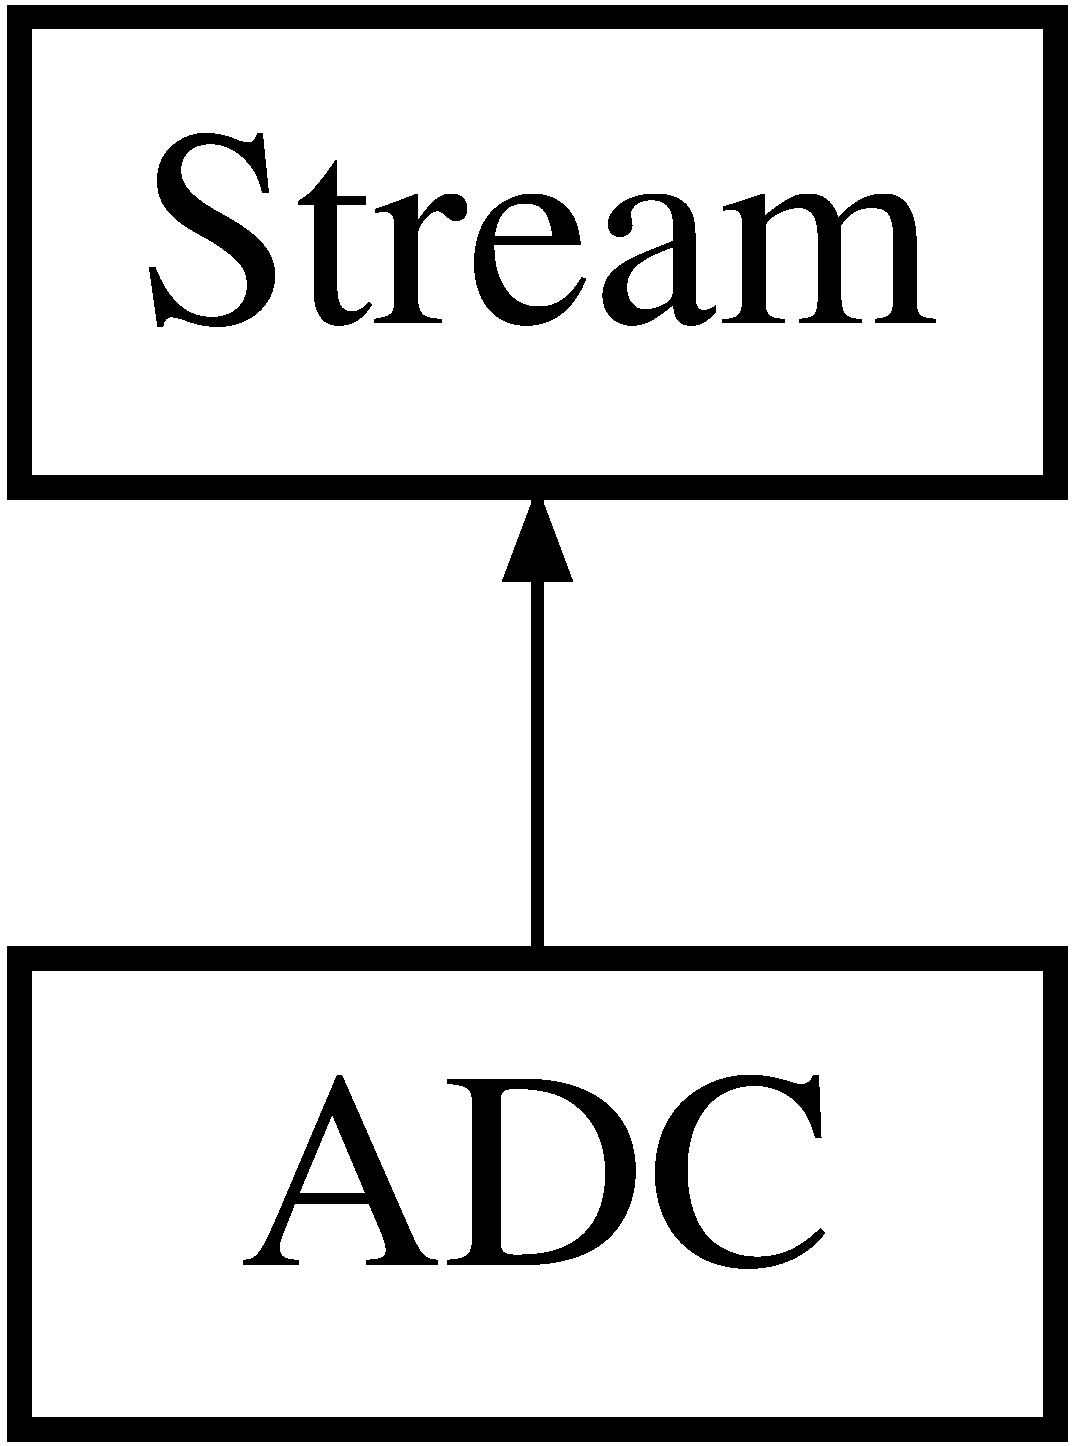
\includegraphics[height=2.000000cm]{class_a_d_c}
\end{center}
\end{figure}
\subsection*{Public Member Functions}
\begin{DoxyCompactItemize}
\item 
\hyperlink{class_a_d_c_a50cb1d4e5bb8e3812732d9efdde4af67}{A\+DC} (const \hyperlink{class_a_d_c}{A\+DC} \&)=delete
\item 
void \hyperlink{class_a_d_c_a8cc7efa85ad7492480bdfd9f49039150}{operator=} (const \hyperlink{class_a_d_c}{A\+DC} \&)=delete
\item 
bool \hyperlink{class_a_d_c_a8264cbf9141f229f5117718e78f01173}{request\+\_\+sample} ()
\end{DoxyCompactItemize}
\subsection*{Static Public Member Functions}
\begin{DoxyCompactItemize}
\item 
static \hyperlink{class_a_d_c}{A\+DC} \& \hyperlink{class_a_d_c_aa9294ebc0b114898aa33d9e09537bdb5}{Get\+Instance} (uint16\+\_\+t adc\+\_\+number, uint8\+\_\+t int\+\_\+pin)
\end{DoxyCompactItemize}
\subsection*{Static Public Attributes}
\begin{DoxyCompactItemize}
\item 
static bool \hyperlink{class_a_d_c_a861d0d9bd4dc73f9811c129548fb9a48}{adc\+\_\+in\+\_\+use} = false
\item 
\hypertarget{class_a_d_c_a472fee5492ee8e10d5baf38b67db18af}{}\label{class_a_d_c_a472fee5492ee8e10d5baf38b67db18af} 
static volatile uint8\+\_\+t $\ast$ {\bfseries adc\+\_\+waiting} = nullptr
\end{DoxyCompactItemize}
\subsection*{Private Member Functions}
\begin{DoxyCompactItemize}
\item 
\hyperlink{class_a_d_c_a0818050dee0dd8789966db0f429ef0bd}{A\+DC} (uint16\+\_\+t address, uint8\+\_\+t int\+\_\+pin)
\end{DoxyCompactItemize}
\subsection*{Private Attributes}
\begin{DoxyCompactItemize}
\item 
\hypertarget{class_a_d_c_aa58c27581281db4bd8537df9ea2b49f2}{}\label{class_a_d_c_aa58c27581281db4bd8537df9ea2b49f2} 
volatile uint8\+\_\+t $\ast$ {\bfseries address}
\end{DoxyCompactItemize}
\subsection*{Static Private Attributes}
\begin{DoxyCompactItemize}
\item 
\hypertarget{class_a_d_c_a6e0562436e7b39f0e53435ed5cc393a3}{}\label{class_a_d_c_a6e0562436e7b39f0e53435ed5cc393a3} 
static uint8\+\_\+t {\bfseries int\+\_\+pin} = 0
\end{DoxyCompactItemize}
\subsection*{Friends}
\begin{DoxyCompactItemize}
\item 
void \hyperlink{class_a_d_c_a8f7964aad4550f29972483135452c811}{I\+N\+T2\+\_\+vect} ()
\end{DoxyCompactItemize}
\subsection*{Additional Inherited Members}


\subsection{Constructor \& Destructor Documentation}
\hypertarget{class_a_d_c_a0818050dee0dd8789966db0f429ef0bd}{}\label{class_a_d_c_a0818050dee0dd8789966db0f429ef0bd} 
\index{A\+DC@{A\+DC}!A\+DC@{A\+DC}}
\index{A\+DC@{A\+DC}!A\+DC@{A\+DC}}
\subsubsection{\texorpdfstring{A\+D\+C()}{ADC()}\hspace{0.1cm}{\footnotesize\ttfamily [1/2]}}
{\footnotesize\ttfamily A\+D\+C\+::\+A\+DC (\begin{DoxyParamCaption}\item[{uint16\+\_\+t}]{address,  }\item[{uint8\+\_\+t}]{int\+\_\+pin }\end{DoxyParamCaption})\hspace{0.3cm}{\ttfamily [private]}}

Constructor for \hyperlink{class_a_d_c}{A\+DC} class. Singleton implementation 
\begin{DoxyParams}{Parameters}
{\em address} & The address the \hyperlink{class_a_d_c}{A\+DC} is located at. Channel on the adc is determined by the L\+SB. We use 0x1404 for channel 1 and 0x1405 for channel 2 \\
\hline
\end{DoxyParams}
\hypertarget{class_a_d_c_a50cb1d4e5bb8e3812732d9efdde4af67}{}\label{class_a_d_c_a50cb1d4e5bb8e3812732d9efdde4af67} 
\index{A\+DC@{A\+DC}!A\+DC@{A\+DC}}
\index{A\+DC@{A\+DC}!A\+DC@{A\+DC}}
\subsubsection{\texorpdfstring{A\+D\+C()}{ADC()}\hspace{0.1cm}{\footnotesize\ttfamily [2/2]}}
{\footnotesize\ttfamily A\+D\+C\+::\+A\+DC (\begin{DoxyParamCaption}\item[{const \hyperlink{class_a_d_c}{A\+DC} \&}]{ }\end{DoxyParamCaption})\hspace{0.3cm}{\ttfamily [delete]}}

Beacause of singleton -\/ makes sure its not copied etc. 

\subsection{Member Function Documentation}
\hypertarget{class_a_d_c_aa9294ebc0b114898aa33d9e09537bdb5}{}\label{class_a_d_c_aa9294ebc0b114898aa33d9e09537bdb5} 
\index{A\+DC@{A\+DC}!Get\+Instance@{Get\+Instance}}
\index{Get\+Instance@{Get\+Instance}!A\+DC@{A\+DC}}
\subsubsection{\texorpdfstring{Get\+Instance()}{GetInstance()}}
{\footnotesize\ttfamily static \hyperlink{class_a_d_c}{A\+DC}\& A\+D\+C\+::\+Get\+Instance (\begin{DoxyParamCaption}\item[{uint16\+\_\+t}]{adc\+\_\+number,  }\item[{uint8\+\_\+t}]{int\+\_\+pin }\end{DoxyParamCaption})\hspace{0.3cm}{\ttfamily [inline]}, {\ttfamily [static]}}

A Singleton implementation of this class. See \hyperlink{class_a_d_c}{A\+D\+C(uint16\+\_\+t address)} for more information. \hypertarget{class_a_d_c_a8cc7efa85ad7492480bdfd9f49039150}{}\label{class_a_d_c_a8cc7efa85ad7492480bdfd9f49039150} 
\index{A\+DC@{A\+DC}!operator=@{operator=}}
\index{operator=@{operator=}!A\+DC@{A\+DC}}
\subsubsection{\texorpdfstring{operator=()}{operator=()}}
{\footnotesize\ttfamily void A\+D\+C\+::operator= (\begin{DoxyParamCaption}\item[{const \hyperlink{class_a_d_c}{A\+DC} \&}]{ }\end{DoxyParamCaption})\hspace{0.3cm}{\ttfamily [delete]}}

Beacause of singleton -\/ makes sure its not copied etc. \hypertarget{class_a_d_c_a8264cbf9141f229f5117718e78f01173}{}\label{class_a_d_c_a8264cbf9141f229f5117718e78f01173} 
\index{A\+DC@{A\+DC}!request\+\_\+sample@{request\+\_\+sample}}
\index{request\+\_\+sample@{request\+\_\+sample}!A\+DC@{A\+DC}}
\subsubsection{\texorpdfstring{request\+\_\+sample()}{request\_sample()}}
{\footnotesize\ttfamily bool A\+D\+C\+::request\+\_\+sample (\begin{DoxyParamCaption}{ }\end{DoxyParamCaption})}

Request the \hyperlink{class_a_d_c}{A\+DC} to get a sample. This sample can be read from the buffer using \hyperlink{class_stream_a6db4180f5834073f992608b856bddca2}{Read\+Byte(uint8\+\_\+t\& byte)}; 

\subsection{Friends And Related Function Documentation}
\hypertarget{class_a_d_c_a8f7964aad4550f29972483135452c811}{}\label{class_a_d_c_a8f7964aad4550f29972483135452c811} 
\index{A\+DC@{A\+DC}!I\+N\+T2\+\_\+vect@{I\+N\+T2\+\_\+vect}}
\index{I\+N\+T2\+\_\+vect@{I\+N\+T2\+\_\+vect}!A\+DC@{A\+DC}}
\subsubsection{\texorpdfstring{I\+N\+T2\+\_\+vect}{INT2\_vect}}
{\footnotesize\ttfamily void I\+N\+T2\+\_\+vect (\begin{DoxyParamCaption}{ }\end{DoxyParamCaption})\hspace{0.3cm}{\ttfamily [friend]}}

The interrupt vector for \hyperlink{class_a_d_c}{A\+DC} done 

\subsection{Member Data Documentation}
\hypertarget{class_a_d_c_a861d0d9bd4dc73f9811c129548fb9a48}{}\label{class_a_d_c_a861d0d9bd4dc73f9811c129548fb9a48} 
\index{A\+DC@{A\+DC}!adc\+\_\+in\+\_\+use@{adc\+\_\+in\+\_\+use}}
\index{adc\+\_\+in\+\_\+use@{adc\+\_\+in\+\_\+use}!A\+DC@{A\+DC}}
\subsubsection{\texorpdfstring{adc\+\_\+in\+\_\+use}{adc\_in\_use}}
{\footnotesize\ttfamily bool A\+D\+C\+::adc\+\_\+in\+\_\+use = false\hspace{0.3cm}{\ttfamily [static]}}

A flag indicating if the \hyperlink{class_a_d_c}{A\+DC} is currently used 

The documentation for this class was generated from the following files\+:\begin{DoxyCompactItemize}
\item 
lib/adc/adc.\+h\item 
lib/adc/adc.\+cpp\end{DoxyCompactItemize}

\hypertarget{class_menu_1_1_controller}{}\section{Menu\+:\+:Controller Class Reference}
\label{class_menu_1_1_controller}\index{Menu\+::\+Controller@{Menu\+::\+Controller}}


{\ttfamily \#include $<$menu.\+h$>$}

\subsection*{Public Member Functions}
\begin{DoxyCompactItemize}
\item 
\hyperlink{class_menu_1_1_controller_afcbda47e43a9753875631f0d4106f604}{Controller} (\hyperlink{class_o_l_e_d}{O\+L\+ED} \&\hyperlink{class_menu_1_1_controller_aaa0388123d9e3bb0d4f546336e2b502d}{oled}, uint8\+\_\+t \hyperlink{class_menu_1_1_controller_a80d614a66d1ffa2612688776842f1f31}{num\+\_\+lines})
\item 
void \hyperlink{class_menu_1_1_controller_a4d270009fff9dfc6baa4433f219626c4}{Control\+Go\+To\+Root} ()
\item 
void \hyperlink{class_menu_1_1_controller_a0dae623388e9bb9e651385d0ef9a2394}{Control\+Go\+To\+Item} (uint8\+\_\+t index)
\item 
void \hyperlink{class_menu_1_1_controller_a9a4c0ccd822f485834ec9abb4133a059}{Control\+Enter\+Sub\+Menu} ()
\item 
void \hyperlink{class_menu_1_1_controller_a8bc1d62574e86a08d5a60652370dd21a}{Control\+Enter\+Sub\+Menu} (uint8\+\_\+t index)
\item 
void \hyperlink{class_menu_1_1_controller_ad4bcb0925c933dce2cceacdbd1b26294}{Control\+Go\+To\+Parent} ()
\item 
void \hyperlink{class_menu_1_1_controller_ab530ec11f04b96254b93961d26152d3c}{Add\+Menu} (\hyperlink{struct_menu_1_1_item}{Item} $\ast$$\ast$items, uint8\+\_\+t length)
\item 
void \hyperlink{class_menu_1_1_controller_ad28e732923bf111fd26a7ea031885f70}{Add\+Menu\+Items} (\hyperlink{struct_menu_1_1_item}{Item} $\ast$$\ast$items, uint8\+\_\+t length)
\item 
void \hyperlink{class_menu_1_1_controller_a777d65ba4f168aed6c1c44022ca4c658}{Add\+Menu\+Item} (\hyperlink{struct_menu_1_1_item}{Item} $\ast$item)
\item 
void \hyperlink{class_menu_1_1_controller_a9e5366f182975680e88749f03d249a0a}{Add\+Menu\+Item} (\hyperlink{struct_menu_1_1_item}{Item} $\ast$item, uint8\+\_\+t index)
\item 
void \hyperlink{class_menu_1_1_controller_a1df8e49520c77372d479903c3ec93341}{Go\+To\+Menu} (\hyperlink{struct_menu_1_1_menu}{Menu} $\ast$menu)
\item 
void \hyperlink{class_menu_1_1_controller_a787911ef46ca1968c2fd667af1f9ac27}{Go\+To\+Root} ()
\item 
void \hyperlink{class_menu_1_1_controller_ab30a038c4e4e3cb102d419c11a6813f6}{Go\+To\+Parent} ()
\item 
void \hyperlink{class_menu_1_1_controller_a9aabc6ba652c29efa7a02e12f51ce0b1}{Select\+Next} ()
\item 
void \hyperlink{class_menu_1_1_controller_a04e3448cfe4341ad7209a9f16bbcb449}{Select\+Previous} ()
\item 
void \hyperlink{class_menu_1_1_controller_a0dda40652b8802a8fe39c1ce61a66f1a}{Execute\+Item} ()
\item 
void \hyperlink{class_menu_1_1_controller_af46abb3d242c76822c0e8ea8ab777fa5}{Render} ()
\end{DoxyCompactItemize}
\subsection*{Private Member Functions}
\begin{DoxyCompactItemize}
\item 
uint8\+\_\+t \hyperlink{class_menu_1_1_controller_a24009cee76b147079041b2130a806027}{Get\+Menu\+Length} (\hyperlink{struct_menu_1_1_menu}{Menu} $\ast$menu)
\item 
void \hyperlink{class_menu_1_1_controller_afa4a1e26efe90dd5d9479bb8c84404b6}{Go\+To\+Item} (uint8\+\_\+t index)
\item 
bool \hyperlink{class_menu_1_1_controller_ad93989bb6a9ed55f67ad5c15e666cf39}{Go\+To\+Next\+Item} ()
\end{DoxyCompactItemize}
\subsection*{Private Attributes}
\begin{DoxyCompactItemize}
\item 
\hyperlink{class_o_l_e_d}{O\+L\+ED} $\ast$ \hyperlink{class_menu_1_1_controller_aaa0388123d9e3bb0d4f546336e2b502d}{oled} = nullptr
\item 
uint8\+\_\+t \hyperlink{class_menu_1_1_controller_a80d614a66d1ffa2612688776842f1f31}{num\+\_\+lines}
\item 
\hyperlink{struct_menu_1_1_menu}{Menu} $\ast$ \hyperlink{class_menu_1_1_controller_a211b6de05f7eed25f3a7f504c42316e0}{root}
\item 
\hyperlink{struct_menu_1_1_menu}{Menu} $\ast$ \hyperlink{class_menu_1_1_controller_a912ad4ad6b2c30e7cddf44547585a909}{current\+\_\+menu\+\_\+control} = nullptr
\item 
\hyperlink{struct_menu_1_1_item}{Item} $\ast$ \hyperlink{class_menu_1_1_controller_a288e26b1efe4fd953b5514de72a1c508}{current\+\_\+item\+\_\+control} = nullptr
\item 
\hyperlink{struct_menu_1_1_menu}{Menu} $\ast$ \hyperlink{class_menu_1_1_controller_a66ffabf19a4423ccca536762f0b9df88}{current\+\_\+menu\+\_\+navigate} = nullptr
\item 
\hyperlink{struct_menu_1_1_item}{Item} $\ast$ \hyperlink{class_menu_1_1_controller_a6dfb1678cc8fd44570806ff680ac27cf}{current\+\_\+item\+\_\+navigate} = nullptr
\item 
uint8\+\_\+t \hyperlink{class_menu_1_1_controller_a86055b66afbad89c5a0b8a0a1713f9d3}{current\+\_\+index\+\_\+navigate} = 0
\item 
uint8\+\_\+t \hyperlink{class_menu_1_1_controller_ab3bdee08f22d55f8fa0cb9e29bb27d66}{current\+\_\+index\+\_\+selected} = 0
\end{DoxyCompactItemize}


\subsection{Detailed Description}
This class contains everything needed to create and manage a menu and display it on an \hyperlink{class_o_l_e_d}{O\+L\+ED}. 

\subsection{Constructor \& Destructor Documentation}
\index{Menu\+::\+Controller@{Menu\+::\+Controller}!Controller@{Controller}}
\index{Controller@{Controller}!Menu\+::\+Controller@{Menu\+::\+Controller}}
\subsubsection[{\texorpdfstring{Controller(\+O\+L\+E\+D \&oled, uint8\+\_\+t num\+\_\+lines)}{Controller(OLED &oled, uint8_t num_lines)}}]{\setlength{\rightskip}{0pt plus 5cm}Menu\+::\+Controller\+::\+Controller (
\begin{DoxyParamCaption}
\item[{{\bf O\+L\+ED} \&}]{oled, }
\item[{uint8\+\_\+t}]{num\+\_\+lines}
\end{DoxyParamCaption}
)}\hypertarget{class_menu_1_1_controller_afcbda47e43a9753875631f0d4106f604}{}\label{class_menu_1_1_controller_afcbda47e43a9753875631f0d4106f604}
Sets up the menu. 
\begin{DoxyParams}{Parameters}
{\em oled} & This is the oled object the menu should use for display. \\
\hline
{\em num\+\_\+lines} & This is the number of lines that the display should use when displaying the menu. \\
\hline
\end{DoxyParams}


\subsection{Member Function Documentation}
\index{Menu\+::\+Controller@{Menu\+::\+Controller}!Add\+Menu@{Add\+Menu}}
\index{Add\+Menu@{Add\+Menu}!Menu\+::\+Controller@{Menu\+::\+Controller}}
\subsubsection[{\texorpdfstring{Add\+Menu(\+Item $\ast$$\ast$items, uint8\+\_\+t length)}{AddMenu(Item **items, uint8_t length)}}]{\setlength{\rightskip}{0pt plus 5cm}void Menu\+::\+Controller\+::\+Add\+Menu (
\begin{DoxyParamCaption}
\item[{{\bf Item} $\ast$$\ast$}]{items, }
\item[{uint8\+\_\+t}]{length}
\end{DoxyParamCaption}
)}\hypertarget{class_menu_1_1_controller_ab530ec11f04b96254b93961d26152d3c}{}\label{class_menu_1_1_controller_ab530ec11f04b96254b93961d26152d3c}
Adds a sub menu to the currently selected item. Assumes an item is selected. Internally it creates a menu, and invokes Add\+Menu\+Item to add the items. Thus you could create an empty menu and add items using Add\+Menu\+Item instead. Do N\+OT use this to create the root menu; it is already made. Use Add\+Menu\+Item to add items to it. 
\begin{DoxyParams}{Parameters}
{\em items} & An array of items to add to the newly created menu. \\
\hline
{\em length} & The length of the array. \\
\hline
\end{DoxyParams}
\index{Menu\+::\+Controller@{Menu\+::\+Controller}!Add\+Menu\+Item@{Add\+Menu\+Item}}
\index{Add\+Menu\+Item@{Add\+Menu\+Item}!Menu\+::\+Controller@{Menu\+::\+Controller}}
\subsubsection[{\texorpdfstring{Add\+Menu\+Item(\+Item $\ast$item)}{AddMenuItem(Item *item)}}]{\setlength{\rightskip}{0pt plus 5cm}void Menu\+::\+Controller\+::\+Add\+Menu\+Item (
\begin{DoxyParamCaption}
\item[{{\bf Item} $\ast$}]{item}
\end{DoxyParamCaption}
)}\hypertarget{class_menu_1_1_controller_a777d65ba4f168aed6c1c44022ca4c658}{}\label{class_menu_1_1_controller_a777d65ba4f168aed6c1c44022ca4c658}
Adds the item after the currently selected item. If no item is selected, the item is inserted as the first item. 
\begin{DoxyParams}{Parameters}
{\em item} & The item to insert. \\
\hline
\end{DoxyParams}
\index{Menu\+::\+Controller@{Menu\+::\+Controller}!Add\+Menu\+Item@{Add\+Menu\+Item}}
\index{Add\+Menu\+Item@{Add\+Menu\+Item}!Menu\+::\+Controller@{Menu\+::\+Controller}}
\subsubsection[{\texorpdfstring{Add\+Menu\+Item(\+Item $\ast$item, uint8\+\_\+t index)}{AddMenuItem(Item *item, uint8_t index)}}]{\setlength{\rightskip}{0pt plus 5cm}void Menu\+::\+Controller\+::\+Add\+Menu\+Item (
\begin{DoxyParamCaption}
\item[{{\bf Item} $\ast$}]{item, }
\item[{uint8\+\_\+t}]{index}
\end{DoxyParamCaption}
)}\hypertarget{class_menu_1_1_controller_a9e5366f182975680e88749f03d249a0a}{}\label{class_menu_1_1_controller_a9e5366f182975680e88749f03d249a0a}
Adds the item at the specified index. Thus index 0 will place it as the first element in the menu. 
\begin{DoxyParams}{Parameters}
{\em item} & The item to insert. \\
\hline
{\em index} & The index the inserted item should have. \\
\hline
\end{DoxyParams}
\index{Menu\+::\+Controller@{Menu\+::\+Controller}!Add\+Menu\+Items@{Add\+Menu\+Items}}
\index{Add\+Menu\+Items@{Add\+Menu\+Items}!Menu\+::\+Controller@{Menu\+::\+Controller}}
\subsubsection[{\texorpdfstring{Add\+Menu\+Items(\+Item $\ast$$\ast$items, uint8\+\_\+t length)}{AddMenuItems(Item **items, uint8_t length)}}]{\setlength{\rightskip}{0pt plus 5cm}void Menu\+::\+Controller\+::\+Add\+Menu\+Items (
\begin{DoxyParamCaption}
\item[{{\bf Item} $\ast$$\ast$}]{items, }
\item[{uint8\+\_\+t}]{length}
\end{DoxyParamCaption}
)}\hypertarget{class_menu_1_1_controller_ad28e732923bf111fd26a7ea031885f70}{}\label{class_menu_1_1_controller_ad28e732923bf111fd26a7ea031885f70}
Internally invokes Add\+Menu\+Item to add the items. Adds to the selected item. 
\begin{DoxyParams}{Parameters}
{\em items} & An array of items to add to the menu. \\
\hline
{\em length} & The length of the array. \\
\hline
\end{DoxyParams}
\index{Menu\+::\+Controller@{Menu\+::\+Controller}!Control\+Enter\+Sub\+Menu@{Control\+Enter\+Sub\+Menu}}
\index{Control\+Enter\+Sub\+Menu@{Control\+Enter\+Sub\+Menu}!Menu\+::\+Controller@{Menu\+::\+Controller}}
\subsubsection[{\texorpdfstring{Control\+Enter\+Sub\+Menu()}{ControlEnterSubMenu()}}]{\setlength{\rightskip}{0pt plus 5cm}void Menu\+::\+Controller\+::\+Control\+Enter\+Sub\+Menu (
\begin{DoxyParamCaption}
{}
\end{DoxyParamCaption}
)}\hypertarget{class_menu_1_1_controller_a9a4c0ccd822f485834ec9abb4133a059}{}\label{class_menu_1_1_controller_a9a4c0ccd822f485834ec9abb4133a059}
Enters the sub menu the selected item links to (\hyperlink{struct_menu_1_1_item_a247e140fed2addf80986ba5a3506b9dd}{Item\+::action}). Assumes the current item has a sub menu... \index{Menu\+::\+Controller@{Menu\+::\+Controller}!Control\+Enter\+Sub\+Menu@{Control\+Enter\+Sub\+Menu}}
\index{Control\+Enter\+Sub\+Menu@{Control\+Enter\+Sub\+Menu}!Menu\+::\+Controller@{Menu\+::\+Controller}}
\subsubsection[{\texorpdfstring{Control\+Enter\+Sub\+Menu(uint8\+\_\+t index)}{ControlEnterSubMenu(uint8_t index)}}]{\setlength{\rightskip}{0pt plus 5cm}void Menu\+::\+Controller\+::\+Control\+Enter\+Sub\+Menu (
\begin{DoxyParamCaption}
\item[{uint8\+\_\+t}]{index}
\end{DoxyParamCaption}
)}\hypertarget{class_menu_1_1_controller_a8bc1d62574e86a08d5a60652370dd21a}{}\label{class_menu_1_1_controller_a8bc1d62574e86a08d5a60652370dd21a}
Same as Control\+Enter\+Sub\+Menu, except accesses the menu item with index index instead of the currently selected item. 
\begin{DoxyParams}{Parameters}
{\em index} & The index of the item whose sub menu will be entered. \\
\hline
\end{DoxyParams}
\index{Menu\+::\+Controller@{Menu\+::\+Controller}!Control\+Go\+To\+Item@{Control\+Go\+To\+Item}}
\index{Control\+Go\+To\+Item@{Control\+Go\+To\+Item}!Menu\+::\+Controller@{Menu\+::\+Controller}}
\subsubsection[{\texorpdfstring{Control\+Go\+To\+Item(uint8\+\_\+t index)}{ControlGoToItem(uint8_t index)}}]{\setlength{\rightskip}{0pt plus 5cm}void Menu\+::\+Controller\+::\+Control\+Go\+To\+Item (
\begin{DoxyParamCaption}
\item[{uint8\+\_\+t}]{index}
\end{DoxyParamCaption}
)}\hypertarget{class_menu_1_1_controller_a0dae623388e9bb9e651385d0ef9a2394}{}\label{class_menu_1_1_controller_a0dae623388e9bb9e651385d0ef9a2394}
Sets the item to be controlled to the item with index index of the selected menu. 
\begin{DoxyParams}{Parameters}
{\em index} & The index of the item to be selected. \\
\hline
\end{DoxyParams}
\index{Menu\+::\+Controller@{Menu\+::\+Controller}!Control\+Go\+To\+Parent@{Control\+Go\+To\+Parent}}
\index{Control\+Go\+To\+Parent@{Control\+Go\+To\+Parent}!Menu\+::\+Controller@{Menu\+::\+Controller}}
\subsubsection[{\texorpdfstring{Control\+Go\+To\+Parent()}{ControlGoToParent()}}]{\setlength{\rightskip}{0pt plus 5cm}void Menu\+::\+Controller\+::\+Control\+Go\+To\+Parent (
\begin{DoxyParamCaption}
{}
\end{DoxyParamCaption}
)}\hypertarget{class_menu_1_1_controller_ad4bcb0925c933dce2cceacdbd1b26294}{}\label{class_menu_1_1_controller_ad4bcb0925c933dce2cceacdbd1b26294}
Sets the menu to be controlled to the parent of the current menu. Assumes the currently selected menu isn\textquotesingle{}t the root menu. \index{Menu\+::\+Controller@{Menu\+::\+Controller}!Control\+Go\+To\+Root@{Control\+Go\+To\+Root}}
\index{Control\+Go\+To\+Root@{Control\+Go\+To\+Root}!Menu\+::\+Controller@{Menu\+::\+Controller}}
\subsubsection[{\texorpdfstring{Control\+Go\+To\+Root()}{ControlGoToRoot()}}]{\setlength{\rightskip}{0pt plus 5cm}void Menu\+::\+Controller\+::\+Control\+Go\+To\+Root (
\begin{DoxyParamCaption}
{}
\end{DoxyParamCaption}
)}\hypertarget{class_menu_1_1_controller_a4d270009fff9dfc6baa4433f219626c4}{}\label{class_menu_1_1_controller_a4d270009fff9dfc6baa4433f219626c4}
Sets the menu to be controlled to root. The item selected will be none. \index{Menu\+::\+Controller@{Menu\+::\+Controller}!Execute\+Item@{Execute\+Item}}
\index{Execute\+Item@{Execute\+Item}!Menu\+::\+Controller@{Menu\+::\+Controller}}
\subsubsection[{\texorpdfstring{Execute\+Item()}{ExecuteItem()}}]{\setlength{\rightskip}{0pt plus 5cm}void Menu\+::\+Controller\+::\+Execute\+Item (
\begin{DoxyParamCaption}
{}
\end{DoxyParamCaption}
)}\hypertarget{class_menu_1_1_controller_a0dda40652b8802a8fe39c1ce61a66f1a}{}\label{class_menu_1_1_controller_a0dda40652b8802a8fe39c1ce61a66f1a}
Executes the currently selected items action (calling cb or entering sub menu). Use this as a handler for navigating the menu (for instance \char`\"{}clicking\char`\"{} an item). \index{Menu\+::\+Controller@{Menu\+::\+Controller}!Get\+Menu\+Length@{Get\+Menu\+Length}}
\index{Get\+Menu\+Length@{Get\+Menu\+Length}!Menu\+::\+Controller@{Menu\+::\+Controller}}
\subsubsection[{\texorpdfstring{Get\+Menu\+Length(\+Menu $\ast$menu)}{GetMenuLength(Menu *menu)}}]{\setlength{\rightskip}{0pt plus 5cm}uint8\+\_\+t Menu\+::\+Controller\+::\+Get\+Menu\+Length (
\begin{DoxyParamCaption}
\item[{{\bf Menu} $\ast$}]{menu}
\end{DoxyParamCaption}
)\hspace{0.3cm}{\ttfamily [private]}}\hypertarget{class_menu_1_1_controller_a24009cee76b147079041b2130a806027}{}\label{class_menu_1_1_controller_a24009cee76b147079041b2130a806027}
This calculates the total length of a menu. It is used to for instance figure out what will be the first displayed menu option so that you cannot try to navigate below the menu. 
\begin{DoxyParams}{Parameters}
{\em menu} & The menu to calculate the length of. \\
\hline
\end{DoxyParams}
\begin{DoxyReturn}{Returns}
The menu length. 
\end{DoxyReturn}
\index{Menu\+::\+Controller@{Menu\+::\+Controller}!Go\+To\+Item@{Go\+To\+Item}}
\index{Go\+To\+Item@{Go\+To\+Item}!Menu\+::\+Controller@{Menu\+::\+Controller}}
\subsubsection[{\texorpdfstring{Go\+To\+Item(uint8\+\_\+t index)}{GoToItem(uint8_t index)}}]{\setlength{\rightskip}{0pt plus 5cm}void Menu\+::\+Controller\+::\+Go\+To\+Item (
\begin{DoxyParamCaption}
\item[{uint8\+\_\+t}]{index}
\end{DoxyParamCaption}
)\hspace{0.3cm}{\ttfamily [private]}}\hypertarget{class_menu_1_1_controller_afa4a1e26efe90dd5d9479bb8c84404b6}{}\label{class_menu_1_1_controller_afa4a1e26efe90dd5d9479bb8c84404b6}
Sets the currently selected navigate item to the item with this item. This will only update the item, not the navigate index. This is because this method is only used to select the item so it can be rendered or its action executed. 
\begin{DoxyParams}{Parameters}
{\em index} & The index of the item to be selected. \\
\hline
\end{DoxyParams}
\index{Menu\+::\+Controller@{Menu\+::\+Controller}!Go\+To\+Menu@{Go\+To\+Menu}}
\index{Go\+To\+Menu@{Go\+To\+Menu}!Menu\+::\+Controller@{Menu\+::\+Controller}}
\subsubsection[{\texorpdfstring{Go\+To\+Menu(\+Menu $\ast$menu)}{GoToMenu(Menu *menu)}}]{\setlength{\rightskip}{0pt plus 5cm}void Menu\+::\+Controller\+::\+Go\+To\+Menu (
\begin{DoxyParamCaption}
\item[{{\bf Menu} $\ast$}]{menu}
\end{DoxyParamCaption}
)}\hypertarget{class_menu_1_1_controller_a1df8e49520c77372d479903c3ec93341}{}\label{class_menu_1_1_controller_a1df8e49520c77372d479903c3ec93341}
Sets the specified menu as the current navigate menu. Thus calling this and rendering the menu will go to this menu. 
\begin{DoxyParams}{Parameters}
{\em menu} & The menu to go to. \\
\hline
\end{DoxyParams}
\index{Menu\+::\+Controller@{Menu\+::\+Controller}!Go\+To\+Next\+Item@{Go\+To\+Next\+Item}}
\index{Go\+To\+Next\+Item@{Go\+To\+Next\+Item}!Menu\+::\+Controller@{Menu\+::\+Controller}}
\subsubsection[{\texorpdfstring{Go\+To\+Next\+Item()}{GoToNextItem()}}]{\setlength{\rightskip}{0pt plus 5cm}bool Menu\+::\+Controller\+::\+Go\+To\+Next\+Item (
\begin{DoxyParamCaption}
{}
\end{DoxyParamCaption}
)\hspace{0.3cm}{\ttfamily [private]}}\hypertarget{class_menu_1_1_controller_ad93989bb6a9ed55f67ad5c15e666cf39}{}\label{class_menu_1_1_controller_ad93989bb6a9ed55f67ad5c15e666cf39}
This will try to set the next item as the navigate item. It does not update the navigate index. \begin{DoxyReturn}{Returns}
Whether there was another menu item. 
\end{DoxyReturn}
\index{Menu\+::\+Controller@{Menu\+::\+Controller}!Go\+To\+Parent@{Go\+To\+Parent}}
\index{Go\+To\+Parent@{Go\+To\+Parent}!Menu\+::\+Controller@{Menu\+::\+Controller}}
\subsubsection[{\texorpdfstring{Go\+To\+Parent()}{GoToParent()}}]{\setlength{\rightskip}{0pt plus 5cm}void Menu\+::\+Controller\+::\+Go\+To\+Parent (
\begin{DoxyParamCaption}
{}
\end{DoxyParamCaption}
)}\hypertarget{class_menu_1_1_controller_ab30a038c4e4e3cb102d419c11a6813f6}{}\label{class_menu_1_1_controller_ab30a038c4e4e3cb102d419c11a6813f6}
Sets the navigation to the parent menu. Used to go one menu up. Use this as a handler for navigating one level up in the menu. \index{Menu\+::\+Controller@{Menu\+::\+Controller}!Go\+To\+Root@{Go\+To\+Root}}
\index{Go\+To\+Root@{Go\+To\+Root}!Menu\+::\+Controller@{Menu\+::\+Controller}}
\subsubsection[{\texorpdfstring{Go\+To\+Root()}{GoToRoot()}}]{\setlength{\rightskip}{0pt plus 5cm}void Menu\+::\+Controller\+::\+Go\+To\+Root (
\begin{DoxyParamCaption}
{}
\end{DoxyParamCaption}
)}\hypertarget{class_menu_1_1_controller_a787911ef46ca1968c2fd667af1f9ac27}{}\label{class_menu_1_1_controller_a787911ef46ca1968c2fd667af1f9ac27}
Sets the currently selected navigate item to the root. Also updates the navigate index and selected index. This is used to return the navigation to the root. Use this as a handler for navigating to the root in the menu. \index{Menu\+::\+Controller@{Menu\+::\+Controller}!Render@{Render}}
\index{Render@{Render}!Menu\+::\+Controller@{Menu\+::\+Controller}}
\subsubsection[{\texorpdfstring{Render()}{Render()}}]{\setlength{\rightskip}{0pt plus 5cm}void Menu\+::\+Controller\+::\+Render (
\begin{DoxyParamCaption}
{}
\end{DoxyParamCaption}
)}\hypertarget{class_menu_1_1_controller_af46abb3d242c76822c0e8ea8ab777fa5}{}\label{class_menu_1_1_controller_af46abb3d242c76822c0e8ea8ab777fa5}
Renders the menu to the screen. A normal use case would be to create the menu, add menus to it. Then bind listeners to the menu controls (e.\+g. buttons or joystick) and render the menu when you want to display it. \index{Menu\+::\+Controller@{Menu\+::\+Controller}!Select\+Next@{Select\+Next}}
\index{Select\+Next@{Select\+Next}!Menu\+::\+Controller@{Menu\+::\+Controller}}
\subsubsection[{\texorpdfstring{Select\+Next()}{SelectNext()}}]{\setlength{\rightskip}{0pt plus 5cm}void Menu\+::\+Controller\+::\+Select\+Next (
\begin{DoxyParamCaption}
{}
\end{DoxyParamCaption}
)}\hypertarget{class_menu_1_1_controller_a9aabc6ba652c29efa7a02e12f51ce0b1}{}\label{class_menu_1_1_controller_a9aabc6ba652c29efa7a02e12f51ce0b1}
Updates the selected index. If there is no next item it will not update anything. Use this as a handler for navigating downwards in the menu. \index{Menu\+::\+Controller@{Menu\+::\+Controller}!Select\+Previous@{Select\+Previous}}
\index{Select\+Previous@{Select\+Previous}!Menu\+::\+Controller@{Menu\+::\+Controller}}
\subsubsection[{\texorpdfstring{Select\+Previous()}{SelectPrevious()}}]{\setlength{\rightskip}{0pt plus 5cm}void Menu\+::\+Controller\+::\+Select\+Previous (
\begin{DoxyParamCaption}
{}
\end{DoxyParamCaption}
)}\hypertarget{class_menu_1_1_controller_a04e3448cfe4341ad7209a9f16bbcb449}{}\label{class_menu_1_1_controller_a04e3448cfe4341ad7209a9f16bbcb449}
Updates the selected index. If there is no previous item it will not update anything. Use this as a handler for navigating upwards in the menu. 

\subsection{Member Data Documentation}
\index{Menu\+::\+Controller@{Menu\+::\+Controller}!current\+\_\+index\+\_\+navigate@{current\+\_\+index\+\_\+navigate}}
\index{current\+\_\+index\+\_\+navigate@{current\+\_\+index\+\_\+navigate}!Menu\+::\+Controller@{Menu\+::\+Controller}}
\subsubsection[{\texorpdfstring{current\+\_\+index\+\_\+navigate}{current_index_navigate}}]{\setlength{\rightskip}{0pt plus 5cm}uint8\+\_\+t Menu\+::\+Controller\+::current\+\_\+index\+\_\+navigate = 0\hspace{0.3cm}{\ttfamily [private]}}\hypertarget{class_menu_1_1_controller_a86055b66afbad89c5a0b8a0a1713f9d3}{}\label{class_menu_1_1_controller_a86055b66afbad89c5a0b8a0a1713f9d3}
This stores the index of the first menu item to be displayed on screen. This will change as the user navigates downwards on a menu higher than the number of lines on the screen. When rendering it will be calculated such that the cursor, if possible, does not end up on the first or last lines of the menu. This ensures the user always sees the next item to be selected before it is selected. \index{Menu\+::\+Controller@{Menu\+::\+Controller}!current\+\_\+index\+\_\+selected@{current\+\_\+index\+\_\+selected}}
\index{current\+\_\+index\+\_\+selected@{current\+\_\+index\+\_\+selected}!Menu\+::\+Controller@{Menu\+::\+Controller}}
\subsubsection[{\texorpdfstring{current\+\_\+index\+\_\+selected}{current_index_selected}}]{\setlength{\rightskip}{0pt plus 5cm}uint8\+\_\+t Menu\+::\+Controller\+::current\+\_\+index\+\_\+selected = 0\hspace{0.3cm}{\ttfamily [private]}}\hypertarget{class_menu_1_1_controller_ab3bdee08f22d55f8fa0cb9e29bb27d66}{}\label{class_menu_1_1_controller_ab3bdee08f22d55f8fa0cb9e29bb27d66}
This stores the index of the currently selected menu item. \index{Menu\+::\+Controller@{Menu\+::\+Controller}!current\+\_\+item\+\_\+control@{current\+\_\+item\+\_\+control}}
\index{current\+\_\+item\+\_\+control@{current\+\_\+item\+\_\+control}!Menu\+::\+Controller@{Menu\+::\+Controller}}
\subsubsection[{\texorpdfstring{current\+\_\+item\+\_\+control}{current_item_control}}]{\setlength{\rightskip}{0pt plus 5cm}{\bf Item}$\ast$ Menu\+::\+Controller\+::current\+\_\+item\+\_\+control = nullptr\hspace{0.3cm}{\ttfamily [private]}}\hypertarget{class_menu_1_1_controller_a288e26b1efe4fd953b5514de72a1c508}{}\label{class_menu_1_1_controller_a288e26b1efe4fd953b5514de72a1c508}
This stores the current item to be controlled. Should point to an item inside of current\+\_\+menu\+\_\+control. \index{Menu\+::\+Controller@{Menu\+::\+Controller}!current\+\_\+item\+\_\+navigate@{current\+\_\+item\+\_\+navigate}}
\index{current\+\_\+item\+\_\+navigate@{current\+\_\+item\+\_\+navigate}!Menu\+::\+Controller@{Menu\+::\+Controller}}
\subsubsection[{\texorpdfstring{current\+\_\+item\+\_\+navigate}{current_item_navigate}}]{\setlength{\rightskip}{0pt plus 5cm}{\bf Item}$\ast$ Menu\+::\+Controller\+::current\+\_\+item\+\_\+navigate = nullptr\hspace{0.3cm}{\ttfamily [private]}}\hypertarget{class_menu_1_1_controller_a6dfb1678cc8fd44570806ff680ac27cf}{}\label{class_menu_1_1_controller_a6dfb1678cc8fd44570806ff680ac27cf}
This stores the item needed to for instance render the menu or execute the action of the item. \index{Menu\+::\+Controller@{Menu\+::\+Controller}!current\+\_\+menu\+\_\+control@{current\+\_\+menu\+\_\+control}}
\index{current\+\_\+menu\+\_\+control@{current\+\_\+menu\+\_\+control}!Menu\+::\+Controller@{Menu\+::\+Controller}}
\subsubsection[{\texorpdfstring{current\+\_\+menu\+\_\+control}{current_menu_control}}]{\setlength{\rightskip}{0pt plus 5cm}{\bf Menu}$\ast$ Menu\+::\+Controller\+::current\+\_\+menu\+\_\+control = nullptr\hspace{0.3cm}{\ttfamily [private]}}\hypertarget{class_menu_1_1_controller_a912ad4ad6b2c30e7cddf44547585a909}{}\label{class_menu_1_1_controller_a912ad4ad6b2c30e7cddf44547585a909}
When administrating the menu (control), you use methods to navigate to the item you want to change (e.\+g. add a menu item). This stores the menu to be controlled. \index{Menu\+::\+Controller@{Menu\+::\+Controller}!current\+\_\+menu\+\_\+navigate@{current\+\_\+menu\+\_\+navigate}}
\index{current\+\_\+menu\+\_\+navigate@{current\+\_\+menu\+\_\+navigate}!Menu\+::\+Controller@{Menu\+::\+Controller}}
\subsubsection[{\texorpdfstring{current\+\_\+menu\+\_\+navigate}{current_menu_navigate}}]{\setlength{\rightskip}{0pt plus 5cm}{\bf Menu}$\ast$ Menu\+::\+Controller\+::current\+\_\+menu\+\_\+navigate = nullptr\hspace{0.3cm}{\ttfamily [private]}}\hypertarget{class_menu_1_1_controller_a66ffabf19a4423ccca536762f0b9df88}{}\label{class_menu_1_1_controller_a66ffabf19a4423ccca536762f0b9df88}
When using the menu (navigate), you use methods to navigate. This stores the menu you are navigating (on screen). \index{Menu\+::\+Controller@{Menu\+::\+Controller}!num\+\_\+lines@{num\+\_\+lines}}
\index{num\+\_\+lines@{num\+\_\+lines}!Menu\+::\+Controller@{Menu\+::\+Controller}}
\subsubsection[{\texorpdfstring{num\+\_\+lines}{num_lines}}]{\setlength{\rightskip}{0pt plus 5cm}uint8\+\_\+t Menu\+::\+Controller\+::num\+\_\+lines\hspace{0.3cm}{\ttfamily [private]}}\hypertarget{class_menu_1_1_controller_a80d614a66d1ffa2612688776842f1f31}{}\label{class_menu_1_1_controller_a80d614a66d1ffa2612688776842f1f31}
Specifies how many lines the menu should use (always uses the whole screen). \index{Menu\+::\+Controller@{Menu\+::\+Controller}!oled@{oled}}
\index{oled@{oled}!Menu\+::\+Controller@{Menu\+::\+Controller}}
\subsubsection[{\texorpdfstring{oled}{oled}}]{\setlength{\rightskip}{0pt plus 5cm}{\bf O\+L\+ED}$\ast$ Menu\+::\+Controller\+::oled = nullptr\hspace{0.3cm}{\ttfamily [private]}}\hypertarget{class_menu_1_1_controller_aaa0388123d9e3bb0d4f546336e2b502d}{}\label{class_menu_1_1_controller_aaa0388123d9e3bb0d4f546336e2b502d}
Pointer to the oled object. \index{Menu\+::\+Controller@{Menu\+::\+Controller}!root@{root}}
\index{root@{root}!Menu\+::\+Controller@{Menu\+::\+Controller}}
\subsubsection[{\texorpdfstring{root}{root}}]{\setlength{\rightskip}{0pt plus 5cm}{\bf Menu}$\ast$ Menu\+::\+Controller\+::root\hspace{0.3cm}{\ttfamily [private]}}\hypertarget{class_menu_1_1_controller_a211b6de05f7eed25f3a7f504c42316e0}{}\label{class_menu_1_1_controller_a211b6de05f7eed25f3a7f504c42316e0}
This is the root menu, in other words the first/main menu. 

The documentation for this class was generated from the following files\+:\begin{DoxyCompactItemize}
\item 
lib/menu/menu.\+h\item 
lib/menu/menu.\+cpp\end{DoxyCompactItemize}

\hypertarget{struct_menu_1_1_item}{}\section{Menu\+:\+:Item Struct Reference}
\label{struct_menu_1_1_item}\index{Menu\+::\+Item@{Menu\+::\+Item}}


Struct containing a sigle menu item.  




{\ttfamily \#include $<$menu.\+h$>$}

\subsection*{Public Member Functions}
\begin{DoxyCompactItemize}
\item 
{\bfseries Item} (char $\ast$\hyperlink{struct_menu_1_1_item_a378723382fc64c752a85ffe6fec9707e}{label}, uint8\+\_\+t \hyperlink{struct_menu_1_1_item_a46749d046bbbde8d5308848d5394c2dc}{label\+\_\+length})\hypertarget{struct_menu_1_1_item_ad87fb2f4d51e4c095b93af5ea4bd2275}{}\label{struct_menu_1_1_item_ad87fb2f4d51e4c095b93af5ea4bd2275}

\end{DoxyCompactItemize}
\subsection*{Public Attributes}
\begin{DoxyCompactItemize}
\item 
char $\ast$ \hyperlink{struct_menu_1_1_item_a378723382fc64c752a85ffe6fec9707e}{label} = nullptr
\item 
uint8\+\_\+t \hyperlink{struct_menu_1_1_item_a46749d046bbbde8d5308848d5394c2dc}{label\+\_\+length}
\item 
void $\ast$ \hyperlink{struct_menu_1_1_item_a247e140fed2addf80986ba5a3506b9dd}{action} = nullptr
\item 
bool \hyperlink{struct_menu_1_1_item_a5c9895a137458b9a12dafd447ac7430b}{has\+\_\+sub\+\_\+menu} = false
\item 
\hyperlink{struct_menu_1_1_item}{Item} $\ast$ \hyperlink{struct_menu_1_1_item_aadcc1e4e824296c6b72ac7d053f06869}{next} = nullptr
\end{DoxyCompactItemize}


\subsection{Detailed Description}
Struct containing a sigle menu item. 

This struct contains all the necessary information about a menu item. 

\subsection{Member Data Documentation}
\index{Menu\+::\+Item@{Menu\+::\+Item}!action@{action}}
\index{action@{action}!Menu\+::\+Item@{Menu\+::\+Item}}
\subsubsection[{\texorpdfstring{action}{action}}]{\setlength{\rightskip}{0pt plus 5cm}void$\ast$ Menu\+::\+Item\+::action = nullptr}\hypertarget{struct_menu_1_1_item_a247e140fed2addf80986ba5a3506b9dd}{}\label{struct_menu_1_1_item_a247e140fed2addf80986ba5a3506b9dd}
The action is a pointer to either the cb (callback) function, or it is a pointer to another menu (for instance a sub menu or the parent menu). \index{Menu\+::\+Item@{Menu\+::\+Item}!has\+\_\+sub\+\_\+menu@{has\+\_\+sub\+\_\+menu}}
\index{has\+\_\+sub\+\_\+menu@{has\+\_\+sub\+\_\+menu}!Menu\+::\+Item@{Menu\+::\+Item}}
\subsubsection[{\texorpdfstring{has\+\_\+sub\+\_\+menu}{has_sub_menu}}]{\setlength{\rightskip}{0pt plus 5cm}bool Menu\+::\+Item\+::has\+\_\+sub\+\_\+menu = false}\hypertarget{struct_menu_1_1_item_a5c9895a137458b9a12dafd447ac7430b}{}\label{struct_menu_1_1_item_a5c9895a137458b9a12dafd447ac7430b}
Decides wether the action points to a sub menu or a cb. \index{Menu\+::\+Item@{Menu\+::\+Item}!label@{label}}
\index{label@{label}!Menu\+::\+Item@{Menu\+::\+Item}}
\subsubsection[{\texorpdfstring{label}{label}}]{\setlength{\rightskip}{0pt plus 5cm}char$\ast$ Menu\+::\+Item\+::label = nullptr}\hypertarget{struct_menu_1_1_item_a378723382fc64c752a85ffe6fec9707e}{}\label{struct_menu_1_1_item_a378723382fc64c752a85ffe6fec9707e}
This is the label that will show up in the menu. \index{Menu\+::\+Item@{Menu\+::\+Item}!label\+\_\+length@{label\+\_\+length}}
\index{label\+\_\+length@{label\+\_\+length}!Menu\+::\+Item@{Menu\+::\+Item}}
\subsubsection[{\texorpdfstring{label\+\_\+length}{label_length}}]{\setlength{\rightskip}{0pt plus 5cm}uint8\+\_\+t Menu\+::\+Item\+::label\+\_\+length}\hypertarget{struct_menu_1_1_item_a46749d046bbbde8d5308848d5394c2dc}{}\label{struct_menu_1_1_item_a46749d046bbbde8d5308848d5394c2dc}
This is the length of the label. \index{Menu\+::\+Item@{Menu\+::\+Item}!next@{next}}
\index{next@{next}!Menu\+::\+Item@{Menu\+::\+Item}}
\subsubsection[{\texorpdfstring{next}{next}}]{\setlength{\rightskip}{0pt plus 5cm}{\bf Item}$\ast$ Menu\+::\+Item\+::next = nullptr}\hypertarget{struct_menu_1_1_item_aadcc1e4e824296c6b72ac7d053f06869}{}\label{struct_menu_1_1_item_aadcc1e4e824296c6b72ac7d053f06869}
This is a pointer to the next menu item in the menu (linked list). 

The documentation for this struct was generated from the following files\+:\begin{DoxyCompactItemize}
\item 
lib/menu/menu.\+h\item 
lib/menu/menu.\+cpp\end{DoxyCompactItemize}

\hypertarget{class_m_c_p2515}{\section{M\-C\-P2515 Class Reference}
\label{class_m_c_p2515}\index{M\-C\-P2515@{M\-C\-P2515}}
}


{\ttfamily \#include $<$mcp2515.\-h$>$}

Inheritance diagram for M\-C\-P2515\-:\begin{figure}[H]
\begin{center}
\leavevmode
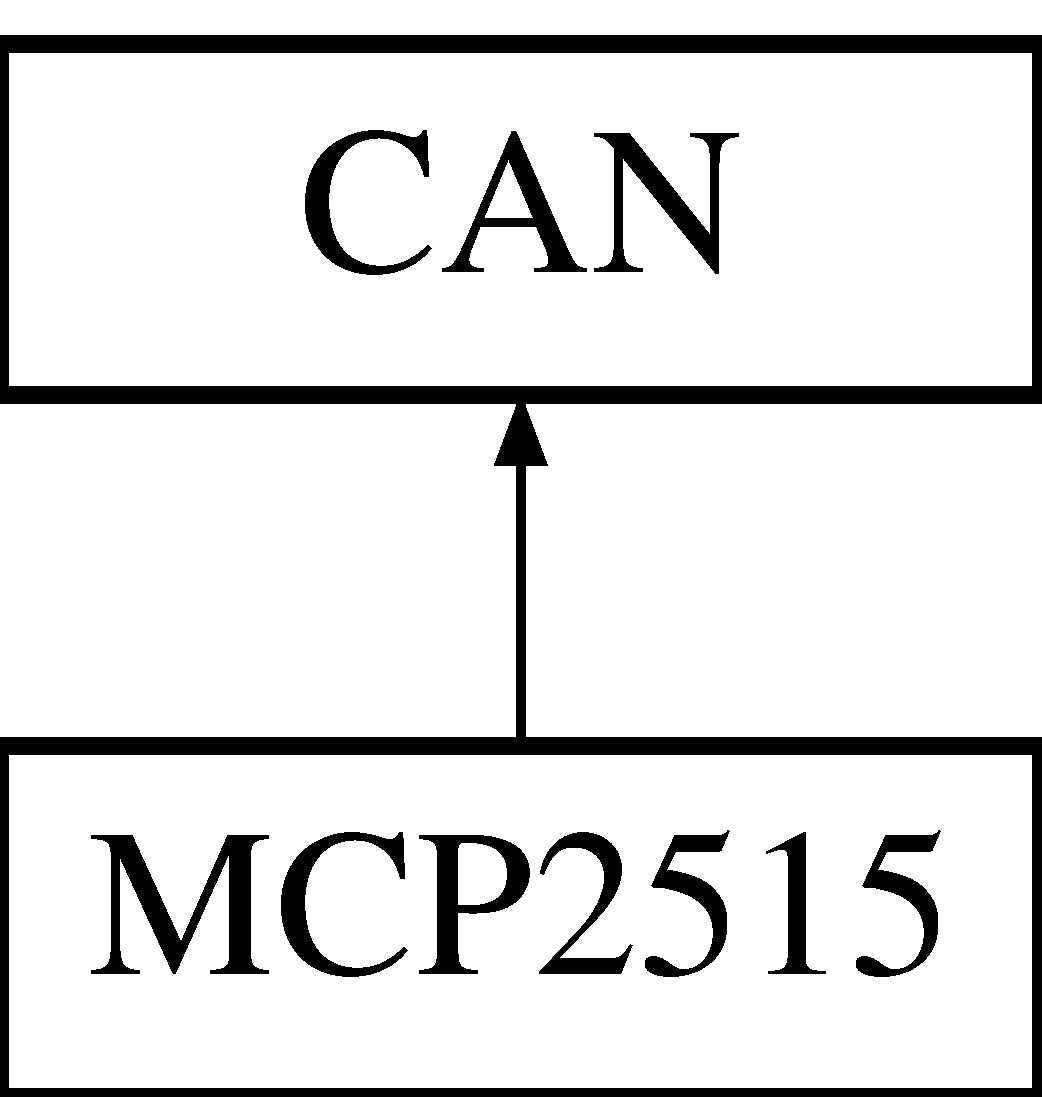
\includegraphics[height=2.000000cm]{class_m_c_p2515}
\end{center}
\end{figure}
\subsection*{Public Member Functions}
\begin{DoxyCompactItemize}
\item 
\hyperlink{class_m_c_p2515_a8cd4111604b740feb758bd4d077f4fb8}{M\-C\-P2515} (const \hyperlink{class_m_c_p2515}{M\-C\-P2515} \&)=delete
\item 
void \hyperlink{class_m_c_p2515_aa8c9fe944f7e6e99feb3f56a1c099a29}{Send\-Message} (\hyperlink{struct_c_a_n___m_e_s_s_a_g_e}{C\-A\-N\-\_\-\-M\-E\-S\-S\-A\-G\-E} \&message)
\item 
void \hyperlink{class_m_c_p2515_a7aac5fdb713b83933391348f1188f2b9}{Set\-Loopback} ()
\item 
void \hyperlink{class_m_c_p2515_a58601a9d30863ebac441d641ddfac44e}{Set\-Normal} ()
\item 
void \hyperlink{class_m_c_p2515_a60a93ccc1a0b21caaba5fda5f88117d2}{Initialize} (\hyperlink{class_s_p_i___n_1_1_s_p_i}{S\-P\-I\-\_\-\-N\-::\-S\-P\-I} $\ast$spi, uint16\-\_\-t identifier)
\end{DoxyCompactItemize}
\subsection*{Static Public Member Functions}
\begin{DoxyCompactItemize}
\item 
static \hyperlink{class_m_c_p2515}{M\-C\-P2515} \& \hyperlink{class_m_c_p2515_a3f53839a9258086fd21e2fc4190de60d}{Get\-Instance} ()
\end{DoxyCompactItemize}
\subsection*{Private Member Functions}
\begin{DoxyCompactItemize}
\item 
void \hyperlink{class_m_c_p2515_a5a218199ca1dfcb25cb95890bc0220fc}{Request\-To\-Send} ()
\item 
void \hyperlink{class_m_c_p2515_adbc005a5975b77b0aef74363f3832f9b}{Write\-To\-Register} (uint8\-\_\-t register\-\_\-address, uint8\-\_\-t byte)
\item 
void \hyperlink{class_m_c_p2515_a09ef6973daccbf868d89986e727cfa1b}{Read\-From\-Register} (uint8\-\_\-t register\-\_\-address, uint8\-\_\-t \&byte)
\item 
void \hyperlink{class_m_c_p2515_aa4d4138b984dc87116cf72ae104acb70}{Reset} ()
\item 
void \hyperlink{class_m_c_p2515_aa9a35fe139adf1fccaaceec561544c14}{Bit\-Modify} (uint8\-\_\-t register\-\_\-address, uint8\-\_\-t mask, uint8\-\_\-t data)
\item 
void \hyperlink{class_m_c_p2515_ae466f10eea5ccf0f36439757d4baf6b5}{Read\-Status} (uint8\-\_\-t \&byte)
\item 
void \hyperlink{class_m_c_p2515_a37771e54c401a0d11b16599f4a3b85df}{Load\-Tx\-Frame} (\hyperlink{struct_c_a_n___m_e_s_s_a_g_e}{C\-A\-N\-\_\-\-M\-E\-S\-S\-A\-G\-E} \&message)
\item 
void \hyperlink{class_m_c_p2515_af6853f82074a0be19d5a0516a959515e}{Rx\-Status} (uint8\-\_\-t \&byte)
\item 
void \hyperlink{class_m_c_p2515_a2035c6707e66a98d92003a3fc99aa784}{Read\-Rx\-Frame} (\hyperlink{struct_c_a_n___m_e_s_s_a_g_e}{C\-A\-N\-\_\-\-M\-E\-S\-S\-A\-G\-E} \&message)
\end{DoxyCompactItemize}
\subsection*{Private Attributes}
\begin{DoxyCompactItemize}
\item 
\hyperlink{class_s_p_i___n_1_1_s_p_i}{S\-P\-I\-\_\-\-N\-::\-S\-P\-I} $\ast$ \hyperlink{class_m_c_p2515_a3a5ca0d606115f1551a06d871606540e}{spi\-\_\-driver}
\item 
volatile bool \hyperlink{class_m_c_p2515_a1418f0f66d9a57659809192552d5ac37}{clear\-\_\-to\-\_\-send} = true
\end{DoxyCompactItemize}
\subsection*{Friends}
\begin{DoxyCompactItemize}
\item 
void \hyperlink{class_m_c_p2515_a3e97befdad3bb95f1da9cf6ff507febe}{M\-C\-P2515\-\_\-\-I\-N\-T} ()
\end{DoxyCompactItemize}
\subsection*{Additional Inherited Members}


\subsection{Detailed Description}
A singleton class which implements the communication between the A\-V\-R and the \hyperlink{class_m_c_p2515}{M\-C\-P2515}. Throughout the documentation of this class, we will refer to the datasheet of the chip. This can be found at \href{http://ww1.microchip.com/downloads/en/DeviceDoc/21801G.pdf}{\tt Microchips site}

The S\-P\-I driver you are using must have meet the following criteria Size of output buffer $>$ 14 bytes  Size of input buffer $>$ 11 bytes 

{\bfseries Please note\-:} This implementation only uses one recieve and transmit buffer. T\-X0 and R\-X0 

\subsection{Constructor \& Destructor Documentation}
\hypertarget{class_m_c_p2515_a8cd4111604b740feb758bd4d077f4fb8}{\index{M\-C\-P2515@{M\-C\-P2515}!M\-C\-P2515@{M\-C\-P2515}}
\index{M\-C\-P2515@{M\-C\-P2515}!MCP2515@{M\-C\-P2515}}
\subsubsection[{M\-C\-P2515}]{\setlength{\rightskip}{0pt plus 5cm}M\-C\-P2515\-::\-M\-C\-P2515 (
\begin{DoxyParamCaption}
\item[{const {\bf M\-C\-P2515} \&}]{}
\end{DoxyParamCaption}
)\hspace{0.3cm}{\ttfamily [delete]}}}\label{class_m_c_p2515_a8cd4111604b740feb758bd4d077f4fb8}
Because of singleton -\/ makes sure its not copied etc. 

\subsection{Member Function Documentation}
\hypertarget{class_m_c_p2515_aa9a35fe139adf1fccaaceec561544c14}{\index{M\-C\-P2515@{M\-C\-P2515}!Bit\-Modify@{Bit\-Modify}}
\index{Bit\-Modify@{Bit\-Modify}!MCP2515@{M\-C\-P2515}}
\subsubsection[{Bit\-Modify}]{\setlength{\rightskip}{0pt plus 5cm}void M\-C\-P2515\-::\-Bit\-Modify (
\begin{DoxyParamCaption}
\item[{uint8\-\_\-t}]{register\-\_\-address, }
\item[{uint8\-\_\-t}]{mask, }
\item[{uint8\-\_\-t}]{data}
\end{DoxyParamCaption}
)\hspace{0.3cm}{\ttfamily [private]}}}\label{class_m_c_p2515_aa9a35fe139adf1fccaaceec561544c14}
Modifies the given \hyperlink{class_m_c_p2515}{M\-C\-P2515} register with a bitmask. Please see \href{http://ww1.microchip.com/downloads/en/DeviceDoc/21801G.pdf}{\tt M\-C\-P2515 datasheet} page 66 
\begin{DoxyParams}{Parameters}
{\em register\-\_\-address} & The address to the \hyperlink{class_m_c_p2515}{M\-C\-P2515} register \\
\hline
{\em mask} & Defines which bits to be modified \\
\hline
{\em data} & The byte to be written \\
\hline
\end{DoxyParams}
\hypertarget{class_m_c_p2515_a3f53839a9258086fd21e2fc4190de60d}{\index{M\-C\-P2515@{M\-C\-P2515}!Get\-Instance@{Get\-Instance}}
\index{Get\-Instance@{Get\-Instance}!MCP2515@{M\-C\-P2515}}
\subsubsection[{Get\-Instance}]{\setlength{\rightskip}{0pt plus 5cm}static {\bf M\-C\-P2515}\& M\-C\-P2515\-::\-Get\-Instance (
\begin{DoxyParamCaption}
{}
\end{DoxyParamCaption}
)\hspace{0.3cm}{\ttfamily [inline]}, {\ttfamily [static]}}}\label{class_m_c_p2515_a3f53839a9258086fd21e2fc4190de60d}
A Singleton implementation of this class \hypertarget{class_m_c_p2515_a60a93ccc1a0b21caaba5fda5f88117d2}{\index{M\-C\-P2515@{M\-C\-P2515}!Initialize@{Initialize}}
\index{Initialize@{Initialize}!MCP2515@{M\-C\-P2515}}
\subsubsection[{Initialize}]{\setlength{\rightskip}{0pt plus 5cm}void M\-C\-P2515\-::\-Initialize (
\begin{DoxyParamCaption}
\item[{{\bf S\-P\-I\-\_\-\-N\-::\-S\-P\-I} $\ast$}]{spi, }
\item[{uint16\-\_\-t}]{identifier}
\end{DoxyParamCaption}
)}}\label{class_m_c_p2515_a60a93ccc1a0b21caaba5fda5f88117d2}
Initializes the \hyperlink{class_m_c_p2515}{M\-C\-P2515} driver. 
\begin{DoxyParams}{Parameters}
{\em spi} & The singleton instance of the S\-P\-I driver \\
\hline
\end{DoxyParams}
\hypertarget{class_m_c_p2515_a37771e54c401a0d11b16599f4a3b85df}{\index{M\-C\-P2515@{M\-C\-P2515}!Load\-Tx\-Frame@{Load\-Tx\-Frame}}
\index{Load\-Tx\-Frame@{Load\-Tx\-Frame}!MCP2515@{M\-C\-P2515}}
\subsubsection[{Load\-Tx\-Frame}]{\setlength{\rightskip}{0pt plus 5cm}void M\-C\-P2515\-::\-Load\-Tx\-Frame (
\begin{DoxyParamCaption}
\item[{{\bf C\-A\-N\-\_\-\-M\-E\-S\-S\-A\-G\-E} \&}]{message}
\end{DoxyParamCaption}
)\hspace{0.3cm}{\ttfamily [private]}}}\label{class_m_c_p2515_a37771e54c401a0d11b16599f4a3b85df}
Loads the transmit frame, i.\-e. sends the \hyperlink{class_c_a_n}{C\-A\-N} data to the \hyperlink{class_m_c_p2515}{M\-C\-P2515} 
\begin{DoxyParams}{Parameters}
{\em message} & The \hyperlink{struct_c_a_n___m_e_s_s_a_g_e}{C\-A\-N\-\_\-\-M\-E\-S\-S\-A\-G\-E} to be loaded into the T\-X frame \\
\hline
\end{DoxyParams}
\hypertarget{class_m_c_p2515_a09ef6973daccbf868d89986e727cfa1b}{\index{M\-C\-P2515@{M\-C\-P2515}!Read\-From\-Register@{Read\-From\-Register}}
\index{Read\-From\-Register@{Read\-From\-Register}!MCP2515@{M\-C\-P2515}}
\subsubsection[{Read\-From\-Register}]{\setlength{\rightskip}{0pt plus 5cm}void M\-C\-P2515\-::\-Read\-From\-Register (
\begin{DoxyParamCaption}
\item[{uint8\-\_\-t}]{register\-\_\-address, }
\item[{uint8\-\_\-t \&}]{byte}
\end{DoxyParamCaption}
)\hspace{0.3cm}{\ttfamily [private]}}}\label{class_m_c_p2515_a09ef6973daccbf868d89986e727cfa1b}
Reads from the given \hyperlink{class_m_c_p2515}{M\-C\-P2515} register 
\begin{DoxyParams}{Parameters}
{\em register\-\_\-address} & The address to the \hyperlink{class_m_c_p2515}{M\-C\-P2515} register \\
\hline
{\em byte} & The byte to be written into \\
\hline
\end{DoxyParams}
\hypertarget{class_m_c_p2515_a2035c6707e66a98d92003a3fc99aa784}{\index{M\-C\-P2515@{M\-C\-P2515}!Read\-Rx\-Frame@{Read\-Rx\-Frame}}
\index{Read\-Rx\-Frame@{Read\-Rx\-Frame}!MCP2515@{M\-C\-P2515}}
\subsubsection[{Read\-Rx\-Frame}]{\setlength{\rightskip}{0pt plus 5cm}void M\-C\-P2515\-::\-Read\-Rx\-Frame (
\begin{DoxyParamCaption}
\item[{{\bf C\-A\-N\-\_\-\-M\-E\-S\-S\-A\-G\-E} \&}]{message}
\end{DoxyParamCaption}
)\hspace{0.3cm}{\ttfamily [private]}}}\label{class_m_c_p2515_a2035c6707e66a98d92003a3fc99aa784}
Reads the Rx\-Frame, i.\-e. retrieves the recieved data 
\begin{DoxyParams}{Parameters}
{\em message} & The message to be written into \\
\hline
\end{DoxyParams}
\hypertarget{class_m_c_p2515_ae466f10eea5ccf0f36439757d4baf6b5}{\index{M\-C\-P2515@{M\-C\-P2515}!Read\-Status@{Read\-Status}}
\index{Read\-Status@{Read\-Status}!MCP2515@{M\-C\-P2515}}
\subsubsection[{Read\-Status}]{\setlength{\rightskip}{0pt plus 5cm}void M\-C\-P2515\-::\-Read\-Status (
\begin{DoxyParamCaption}
\item[{uint8\-\_\-t \&}]{byte}
\end{DoxyParamCaption}
)\hspace{0.3cm}{\ttfamily [private]}}}\label{class_m_c_p2515_ae466f10eea5ccf0f36439757d4baf6b5}
Gets the status byte from the \hyperlink{class_m_c_p2515}{M\-C\-P2515}. Please see \href{http://ww1.microchip.com/downloads/en/DeviceDoc/21801G.pdf}{\tt M\-C\-P2515 datasheet} page 65, {\itshape R\-E\-A\-D S\-T\-A\-T\-U\-S instruction} 
\begin{DoxyParams}{Parameters}
{\em byte} & The byte to be written into \\
\hline
\end{DoxyParams}
\hypertarget{class_m_c_p2515_a5a218199ca1dfcb25cb95890bc0220fc}{\index{M\-C\-P2515@{M\-C\-P2515}!Request\-To\-Send@{Request\-To\-Send}}
\index{Request\-To\-Send@{Request\-To\-Send}!MCP2515@{M\-C\-P2515}}
\subsubsection[{Request\-To\-Send}]{\setlength{\rightskip}{0pt plus 5cm}void M\-C\-P2515\-::\-Request\-To\-Send (
\begin{DoxyParamCaption}
{}
\end{DoxyParamCaption}
)\hspace{0.3cm}{\ttfamily [private]}}}\label{class_m_c_p2515_a5a218199ca1dfcb25cb95890bc0220fc}
Sends a R\-T\-S (Request to Send) signal to the \hyperlink{class_m_c_p2515}{M\-C\-P2515}. \hypertarget{class_m_c_p2515_aa4d4138b984dc87116cf72ae104acb70}{\index{M\-C\-P2515@{M\-C\-P2515}!Reset@{Reset}}
\index{Reset@{Reset}!MCP2515@{M\-C\-P2515}}
\subsubsection[{Reset}]{\setlength{\rightskip}{0pt plus 5cm}void M\-C\-P2515\-::\-Reset (
\begin{DoxyParamCaption}
{}
\end{DoxyParamCaption}
)\hspace{0.3cm}{\ttfamily [private]}}}\label{class_m_c_p2515_aa4d4138b984dc87116cf72ae104acb70}
Sends a reset command to the \hyperlink{class_m_c_p2515}{M\-C\-P2515} thorugh the S\-P\-I interace (hardware reset not connected). Will put the \hyperlink{class_m_c_p2515}{M\-C\-P2515} in config mode. \hypertarget{class_m_c_p2515_af6853f82074a0be19d5a0516a959515e}{\index{M\-C\-P2515@{M\-C\-P2515}!Rx\-Status@{Rx\-Status}}
\index{Rx\-Status@{Rx\-Status}!MCP2515@{M\-C\-P2515}}
\subsubsection[{Rx\-Status}]{\setlength{\rightskip}{0pt plus 5cm}void M\-C\-P2515\-::\-Rx\-Status (
\begin{DoxyParamCaption}
\item[{uint8\-\_\-t \&}]{byte}
\end{DoxyParamCaption}
)\hspace{0.3cm}{\ttfamily [private]}}}\label{class_m_c_p2515_af6853f82074a0be19d5a0516a959515e}
Gets the Rx\-Status byte from the \hyperlink{class_m_c_p2515}{M\-C\-P2515}. Please see \href{http://ww1.microchip.com/downloads/en/DeviceDoc/21801G.pdf}{\tt M\-C\-P2515 datasheet} page 66, {\itshape R\-X S\-T\-A\-T\-U\-S instruction} 
\begin{DoxyParams}{Parameters}
{\em byte} & The byte to be written into \\
\hline
\end{DoxyParams}
\hypertarget{class_m_c_p2515_aa8c9fe944f7e6e99feb3f56a1c099a29}{\index{M\-C\-P2515@{M\-C\-P2515}!Send\-Message@{Send\-Message}}
\index{Send\-Message@{Send\-Message}!MCP2515@{M\-C\-P2515}}
\subsubsection[{Send\-Message}]{\setlength{\rightskip}{0pt plus 5cm}void M\-C\-P2515\-::\-Send\-Message (
\begin{DoxyParamCaption}
\item[{{\bf C\-A\-N\-\_\-\-M\-E\-S\-S\-A\-G\-E} \&}]{message}
\end{DoxyParamCaption}
)\hspace{0.3cm}{\ttfamily [virtual]}}}\label{class_m_c_p2515_aa8c9fe944f7e6e99feb3f56a1c099a29}
Sends a \hyperlink{class_c_a_n}{C\-A\-N} message 
\begin{DoxyParams}{Parameters}
{\em message} & The \hyperlink{class_c_a_n}{C\-A\-N} message to be sent \\
\hline
\end{DoxyParams}


Implements \hyperlink{class_c_a_n}{C\-A\-N}.

\hypertarget{class_m_c_p2515_a7aac5fdb713b83933391348f1188f2b9}{\index{M\-C\-P2515@{M\-C\-P2515}!Set\-Loopback@{Set\-Loopback}}
\index{Set\-Loopback@{Set\-Loopback}!MCP2515@{M\-C\-P2515}}
\subsubsection[{Set\-Loopback}]{\setlength{\rightskip}{0pt plus 5cm}void M\-C\-P2515\-::\-Set\-Loopback (
\begin{DoxyParamCaption}
{}
\end{DoxyParamCaption}
)}}\label{class_m_c_p2515_a7aac5fdb713b83933391348f1188f2b9}
Initiates the loopback mode of the \hyperlink{class_m_c_p2515}{M\-C\-P2515}. Please consult the \href{http://ww1.microchip.com/downloads/en/DeviceDoc/21801G.pdf}{\tt M\-C\-P2515 datasheet} \hypertarget{class_m_c_p2515_a58601a9d30863ebac441d641ddfac44e}{\index{M\-C\-P2515@{M\-C\-P2515}!Set\-Normal@{Set\-Normal}}
\index{Set\-Normal@{Set\-Normal}!MCP2515@{M\-C\-P2515}}
\subsubsection[{Set\-Normal}]{\setlength{\rightskip}{0pt plus 5cm}void M\-C\-P2515\-::\-Set\-Normal (
\begin{DoxyParamCaption}
{}
\end{DoxyParamCaption}
)}}\label{class_m_c_p2515_a58601a9d30863ebac441d641ddfac44e}
Initiates the normal mode of the \hyperlink{class_m_c_p2515}{M\-C\-P2515}. Please consult the \href{http://ww1.microchip.com/downloads/en/DeviceDoc/21801G.pdf}{\tt M\-C\-P2515 datasheet} \hypertarget{class_m_c_p2515_adbc005a5975b77b0aef74363f3832f9b}{\index{M\-C\-P2515@{M\-C\-P2515}!Write\-To\-Register@{Write\-To\-Register}}
\index{Write\-To\-Register@{Write\-To\-Register}!MCP2515@{M\-C\-P2515}}
\subsubsection[{Write\-To\-Register}]{\setlength{\rightskip}{0pt plus 5cm}void M\-C\-P2515\-::\-Write\-To\-Register (
\begin{DoxyParamCaption}
\item[{uint8\-\_\-t}]{register\-\_\-address, }
\item[{uint8\-\_\-t}]{byte}
\end{DoxyParamCaption}
)\hspace{0.3cm}{\ttfamily [private]}}}\label{class_m_c_p2515_adbc005a5975b77b0aef74363f3832f9b}
Writes to the given \hyperlink{class_m_c_p2515}{M\-C\-P2515} register 
\begin{DoxyParams}{Parameters}
{\em register\-\_\-address} & The address to the \hyperlink{class_m_c_p2515}{M\-C\-P2515} register \\
\hline
{\em byte} & The byte to be written to the given register \\
\hline
\end{DoxyParams}


\subsection{Friends And Related Function Documentation}
\hypertarget{class_m_c_p2515_a3e97befdad3bb95f1da9cf6ff507febe}{\index{M\-C\-P2515@{M\-C\-P2515}!M\-C\-P2515\-\_\-\-I\-N\-T@{M\-C\-P2515\-\_\-\-I\-N\-T}}
\index{M\-C\-P2515\-\_\-\-I\-N\-T@{M\-C\-P2515\-\_\-\-I\-N\-T}!MCP2515@{M\-C\-P2515}}
\subsubsection[{M\-C\-P2515\-\_\-\-I\-N\-T}]{\setlength{\rightskip}{0pt plus 5cm}void M\-C\-P2515\-\_\-\-I\-N\-T (
\begin{DoxyParamCaption}
{}
\end{DoxyParamCaption}
)\hspace{0.3cm}{\ttfamily [friend]}}}\label{class_m_c_p2515_a3e97befdad3bb95f1da9cf6ff507febe}
The \hyperlink{class_m_c_p2515}{M\-C\-P2515} interrupt handler 

\subsection{Member Data Documentation}
\hypertarget{class_m_c_p2515_a1418f0f66d9a57659809192552d5ac37}{\index{M\-C\-P2515@{M\-C\-P2515}!clear\-\_\-to\-\_\-send@{clear\-\_\-to\-\_\-send}}
\index{clear\-\_\-to\-\_\-send@{clear\-\_\-to\-\_\-send}!MCP2515@{M\-C\-P2515}}
\subsubsection[{clear\-\_\-to\-\_\-send}]{\setlength{\rightskip}{0pt plus 5cm}volatile bool M\-C\-P2515\-::clear\-\_\-to\-\_\-send = true\hspace{0.3cm}{\ttfamily [private]}}}\label{class_m_c_p2515_a1418f0f66d9a57659809192552d5ac37}
Flag indicating wether or not you can load the T\-X frame. \hypertarget{class_m_c_p2515_a3a5ca0d606115f1551a06d871606540e}{\index{M\-C\-P2515@{M\-C\-P2515}!spi\-\_\-driver@{spi\-\_\-driver}}
\index{spi\-\_\-driver@{spi\-\_\-driver}!MCP2515@{M\-C\-P2515}}
\subsubsection[{spi\-\_\-driver}]{\setlength{\rightskip}{0pt plus 5cm}{\bf S\-P\-I\-\_\-\-N\-::\-S\-P\-I}$\ast$ M\-C\-P2515\-::spi\-\_\-driver\hspace{0.3cm}{\ttfamily [private]}}}\label{class_m_c_p2515_a3a5ca0d606115f1551a06d871606540e}
The S\-P\-I Driver the \hyperlink{class_m_c_p2515}{M\-C\-P2515} uses. 

The documentation for this class was generated from the following files\-:\begin{DoxyCompactItemize}
\item 
lib/mcp2515/mcp2515.\-h\item 
lib/mcp2515/mcp2515.\-cpp\end{DoxyCompactItemize}

\hypertarget{struct_menu_1_1_menu}{}\section{Menu\+:\+:Menu Struct Reference}
\label{struct_menu_1_1_menu}\index{Menu\+::\+Menu@{Menu\+::\+Menu}}


Contains all necessary information about a menu (which could be a sub menu).  




{\ttfamily \#include $<$menu.\+h$>$}

\subsection*{Public Attributes}
\begin{DoxyCompactItemize}
\item 
\hyperlink{struct_menu_1_1_menu}{Menu} $\ast$ \hyperlink{struct_menu_1_1_menu_accedb5340f42f80cf0876b4d1e4df512}{parent} = nullptr
\item 
\hyperlink{struct_menu_1_1_item}{Item} $\ast$ \hyperlink{struct_menu_1_1_menu_aa9cb1f287490ac21ebac38e997c21af0}{first} = nullptr
\end{DoxyCompactItemize}


\subsection{Detailed Description}
Contains all necessary information about a menu (which could be a sub menu). 

\subsection{Member Data Documentation}
\hypertarget{struct_menu_1_1_menu_aa9cb1f287490ac21ebac38e997c21af0}{}\label{struct_menu_1_1_menu_aa9cb1f287490ac21ebac38e997c21af0} 
\index{Menu\+::\+Menu@{Menu\+::\+Menu}!first@{first}}
\index{first@{first}!Menu\+::\+Menu@{Menu\+::\+Menu}}
\subsubsection{\texorpdfstring{first}{first}}
{\footnotesize\ttfamily \hyperlink{struct_menu_1_1_item}{Item}$\ast$ Menu\+::\+Menu\+::first = nullptr}

This is the first menu item in the menu. \hypertarget{struct_menu_1_1_menu_accedb5340f42f80cf0876b4d1e4df512}{}\label{struct_menu_1_1_menu_accedb5340f42f80cf0876b4d1e4df512} 
\index{Menu\+::\+Menu@{Menu\+::\+Menu}!parent@{parent}}
\index{parent@{parent}!Menu\+::\+Menu@{Menu\+::\+Menu}}
\subsubsection{\texorpdfstring{parent}{parent}}
{\footnotesize\ttfamily \hyperlink{struct_menu_1_1_menu}{Menu}$\ast$ Menu\+::\+Menu\+::parent = nullptr}

If it is a sub menu, this points to its parent menu. Else it is nullptr. 

The documentation for this struct was generated from the following file\+:\begin{DoxyCompactItemize}
\item 
lib/menu/menu.\+h\end{DoxyCompactItemize}

\hypertarget{class_o_l_e_d}{}\section{O\+L\+ED Class Reference}
\label{class_o_l_e_d}\index{O\+L\+ED@{O\+L\+ED}}


An interface to communicate with the \hyperlink{class_o_l_e_d}{O\+L\+ED} display.  




{\ttfamily \#include $<$oled.\+h$>$}

Inheritance diagram for O\+L\+ED\+:\begin{figure}[H]
\begin{center}
\leavevmode
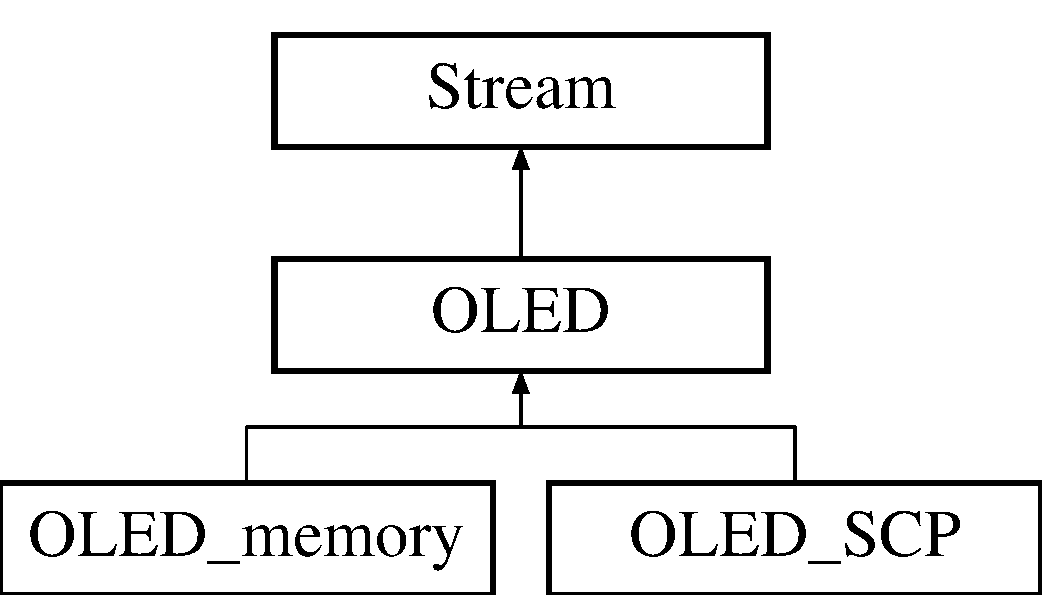
\includegraphics[height=3.000000cm]{class_o_l_e_d}
\end{center}
\end{figure}
\subsection*{Public Member Functions}
\begin{DoxyCompactItemize}
\item 
void \hyperlink{class_o_l_e_d_a2c8205c8eac9d7a2b181657561e9b4d2}{Init} (uint8\+\_\+t width, uint8\+\_\+t height)
\item 
void \hyperlink{class_o_l_e_d_a8d314130676b104ed959b92ab4bac25e}{Go\+To\+Line} (uint8\+\_\+t line)
\item 
void \hyperlink{class_o_l_e_d_a6c7bb1fc91b3e574a275f90643da140a}{Clear} ()
\item 
void \hyperlink{class_o_l_e_d_a3a571f5ea7a183fa14932cd5b2c423eb}{Clear\+Line} ()
\item 
void \hyperlink{class_o_l_e_d_a7fa307269dbd2e80a6e48a1442df83d2}{Write\+Byte} (uint8\+\_\+t page, uint8\+\_\+t column, uint8\+\_\+t byte)
\item 
void \hyperlink{class_o_l_e_d_a7fffc17a5439300d361414c15a7a2dbe}{Write\+Byte\+Array} (uint8\+\_\+t page, uint8\+\_\+t column, uint8\+\_\+t $\ast$byte\+\_\+array, uint8\+\_\+t length)
\item 
void \hyperlink{class_o_l_e_d_a3efa34861b4ae0bc5323f6b7cf1d8a01}{Repaint} ()
\item 
void \hyperlink{class_o_l_e_d_aa3c88e19f05340036ea5ac9e2d1ea5dc}{Set\+Number\+Of\+Lines} (uint8\+\_\+t \hyperlink{class_o_l_e_d_a9ea1c55112deede1a61142af276a6bc9}{number\+\_\+of\+\_\+lines})
\item 
void \hyperlink{class_o_l_e_d_a3cb468f16387343f6db387a86cded8af}{Write\+Bitmap} (uint8\+\_\+t $\ast$$\ast$pixels, uint8\+\_\+t bitmap\+\_\+width, uint8\+\_\+t bitmap\+\_\+height, uint8\+\_\+t x, uint8\+\_\+t y, bool is\+\_\+progmem)
\item 
void \hyperlink{class_o_l_e_d_abe6073c961cadc4c9b693eb8dc8198bd}{Set\+Font} (uint8\+\_\+t $\ast$\hyperlink{class_o_l_e_d_a29ab86a4a73f4d343bf1810927f0911d}{font}, uint8\+\_\+t width, uint8\+\_\+t height)
\item 
void \hyperlink{class_o_l_e_d_a0ffccb4fd874b997c869c5d511f76df8}{Write\+Line} (char $\ast$string, uint8\+\_\+t length, uint8\+\_\+t line, uint8\+\_\+t offset)
\item 
uint8\+\_\+t \hyperlink{class_o_l_e_d_a5b6d41d5d699998f54ea6e3b6562ac5b}{Get\+Y\+Coordinate\+From\+Line\+Number} (uint8\+\_\+t line)
\item 
uint8\+\_\+t \hyperlink{class_o_l_e_d_a7bb08915b685741c60bdccdd47781560}{Get\+Max\+Line\+Characters} ()
\end{DoxyCompactItemize}
\subsection*{Protected Member Functions}
\begin{DoxyCompactItemize}
\item 
\hyperlink{class_o_l_e_d_a8eabf371b5642d99800adb759dab27fd}{O\+L\+ED} ()
\item 
virtual void \hyperlink{class_o_l_e_d_a044fdff65656804114d1d39d766099a2}{Write\+Byte\+To\+O\+L\+ED} (volatile uint8\+\_\+t $\ast$address, uint8\+\_\+t data)
\item 
void \hyperlink{class_o_l_e_d_a3bd2f2f05568441e1e0533eaf0db58f8}{Get\+Bitmap\+For\+Character} (char character, uint8\+\_\+t $\ast$\&character\+\_\+bitmap)
\end{DoxyCompactItemize}
\subsection*{Protected Attributes}
\begin{DoxyCompactItemize}
\item 
uint8\+\_\+t \hyperlink{class_o_l_e_d_aebd62601be5e2ceef6295721f17fc013}{current\+\_\+line} = 0
\item 
uint8\+\_\+t \hyperlink{class_o_l_e_d_a2e9305cb3341509bb62d61f33cae76fd}{display\+\_\+width} = 0
\item 
uint8\+\_\+t \hyperlink{class_o_l_e_d_add08b51dec0ffeebcba7902c3bd4aeea}{display\+\_\+height} = 0
\item 
uint8\+\_\+t \hyperlink{class_o_l_e_d_aaac99b0eb4e9dfe92b8571488dc89288}{number\+\_\+of\+\_\+pages} = 0
\item 
uint8\+\_\+t \hyperlink{class_o_l_e_d_a9ea1c55112deede1a61142af276a6bc9}{number\+\_\+of\+\_\+lines} = 0
\item 
volatile uint8\+\_\+t $\ast$ \hyperlink{class_o_l_e_d_af0a85ccd0274347b8c1ac77d298a14cf}{oled\+\_\+command} = (volatile uint8\+\_\+t$\ast$)0x8000
\item 
volatile uint8\+\_\+t $\ast$ \hyperlink{class_o_l_e_d_a1bc54d49808f92ddfc354511b692df6f}{oled\+\_\+data} = (volatile uint8\+\_\+t$\ast$)0x8100
\item 
uint8\+\_\+t $\ast$$\ast$ \hyperlink{class_o_l_e_d_a9d32e21189940afba24deab0a2bc0126}{matrix}
\item 
uint8\+\_\+t \hyperlink{class_o_l_e_d_a6ddac7b826eccac8c682c5246ef52b29}{pixels\+\_\+per\+\_\+line}
\item 
uint8\+\_\+t $\ast$ \hyperlink{class_o_l_e_d_a29ab86a4a73f4d343bf1810927f0911d}{font} = nullptr
\item 
uint8\+\_\+t \hyperlink{class_o_l_e_d_a3c9ea103adf6c860a2534135e9a25ba8}{font\+\_\+width}
\item 
uint8\+\_\+t \hyperlink{class_o_l_e_d_a85b91421932866dea031921799ba83a3}{font\+\_\+height}
\end{DoxyCompactItemize}


\subsection{Detailed Description}
An interface to communicate with the \hyperlink{class_o_l_e_d}{O\+L\+ED} display. 

\subsection{Constructor \& Destructor Documentation}
\hypertarget{class_o_l_e_d_a8eabf371b5642d99800adb759dab27fd}{}\label{class_o_l_e_d_a8eabf371b5642d99800adb759dab27fd} 
\index{O\+L\+ED@{O\+L\+ED}!O\+L\+ED@{O\+L\+ED}}
\index{O\+L\+ED@{O\+L\+ED}!O\+L\+ED@{O\+L\+ED}}
\subsubsection{\texorpdfstring{O\+L\+E\+D()}{OLED()}}
{\footnotesize\ttfamily O\+L\+E\+D\+::\+O\+L\+ED (\begin{DoxyParamCaption}{ }\end{DoxyParamCaption})\hspace{0.3cm}{\ttfamily [protected]}}

Singleton constructor. 

\subsection{Member Function Documentation}
\hypertarget{class_o_l_e_d_a6c7bb1fc91b3e574a275f90643da140a}{}\label{class_o_l_e_d_a6c7bb1fc91b3e574a275f90643da140a} 
\index{O\+L\+ED@{O\+L\+ED}!Clear@{Clear}}
\index{Clear@{Clear}!O\+L\+ED@{O\+L\+ED}}
\subsubsection{\texorpdfstring{Clear()}{Clear()}}
{\footnotesize\ttfamily void O\+L\+E\+D\+::\+Clear (\begin{DoxyParamCaption}{ }\end{DoxyParamCaption})}

Clears the whole screen. \hypertarget{class_o_l_e_d_a3a571f5ea7a183fa14932cd5b2c423eb}{}\label{class_o_l_e_d_a3a571f5ea7a183fa14932cd5b2c423eb} 
\index{O\+L\+ED@{O\+L\+ED}!Clear\+Line@{Clear\+Line}}
\index{Clear\+Line@{Clear\+Line}!O\+L\+ED@{O\+L\+ED}}
\subsubsection{\texorpdfstring{Clear\+Line()}{ClearLine()}}
{\footnotesize\ttfamily void O\+L\+E\+D\+::\+Clear\+Line (\begin{DoxyParamCaption}{ }\end{DoxyParamCaption})}

Clears the current line. \hypertarget{class_o_l_e_d_a3bd2f2f05568441e1e0533eaf0db58f8}{}\label{class_o_l_e_d_a3bd2f2f05568441e1e0533eaf0db58f8} 
\index{O\+L\+ED@{O\+L\+ED}!Get\+Bitmap\+For\+Character@{Get\+Bitmap\+For\+Character}}
\index{Get\+Bitmap\+For\+Character@{Get\+Bitmap\+For\+Character}!O\+L\+ED@{O\+L\+ED}}
\subsubsection{\texorpdfstring{Get\+Bitmap\+For\+Character()}{GetBitmapForCharacter()}}
{\footnotesize\ttfamily void O\+L\+E\+D\+::\+Get\+Bitmap\+For\+Character (\begin{DoxyParamCaption}\item[{char}]{character,  }\item[{uint8\+\_\+t $\ast$\&}]{character\+\_\+bitmap }\end{DoxyParamCaption})\hspace{0.3cm}{\ttfamily [protected]}}

Fetches a pointer to P\+R\+O\+G\+M\+EM for the bitmap for the given font and character. Emphasis on that it points to P\+R\+O\+G\+M\+EM. \hypertarget{class_o_l_e_d_a7bb08915b685741c60bdccdd47781560}{}\label{class_o_l_e_d_a7bb08915b685741c60bdccdd47781560} 
\index{O\+L\+ED@{O\+L\+ED}!Get\+Max\+Line\+Characters@{Get\+Max\+Line\+Characters}}
\index{Get\+Max\+Line\+Characters@{Get\+Max\+Line\+Characters}!O\+L\+ED@{O\+L\+ED}}
\subsubsection{\texorpdfstring{Get\+Max\+Line\+Characters()}{GetMaxLineCharacters()}}
{\footnotesize\ttfamily uint8\+\_\+t O\+L\+E\+D\+::\+Get\+Max\+Line\+Characters (\begin{DoxyParamCaption}{ }\end{DoxyParamCaption})}

Returns how wide a line is in characters. \begin{DoxyReturn}{Returns}
How wide a line is in characters. 
\end{DoxyReturn}
\hypertarget{class_o_l_e_d_a5b6d41d5d699998f54ea6e3b6562ac5b}{}\label{class_o_l_e_d_a5b6d41d5d699998f54ea6e3b6562ac5b} 
\index{O\+L\+ED@{O\+L\+ED}!Get\+Y\+Coordinate\+From\+Line\+Number@{Get\+Y\+Coordinate\+From\+Line\+Number}}
\index{Get\+Y\+Coordinate\+From\+Line\+Number@{Get\+Y\+Coordinate\+From\+Line\+Number}!O\+L\+ED@{O\+L\+ED}}
\subsubsection{\texorpdfstring{Get\+Y\+Coordinate\+From\+Line\+Number()}{GetYCoordinateFromLineNumber()}}
{\footnotesize\ttfamily uint8\+\_\+t O\+L\+E\+D\+::\+Get\+Y\+Coordinate\+From\+Line\+Number (\begin{DoxyParamCaption}\item[{uint8\+\_\+t}]{line }\end{DoxyParamCaption})}

Returns the y coordinate of the line. 
\begin{DoxyParams}{Parameters}
{\em line} & The line to find the y coordinate of. \\
\hline
\end{DoxyParams}
\begin{DoxyReturn}{Returns}
The y coordinate of the line. 
\end{DoxyReturn}
\hypertarget{class_o_l_e_d_a8d314130676b104ed959b92ab4bac25e}{}\label{class_o_l_e_d_a8d314130676b104ed959b92ab4bac25e} 
\index{O\+L\+ED@{O\+L\+ED}!Go\+To\+Line@{Go\+To\+Line}}
\index{Go\+To\+Line@{Go\+To\+Line}!O\+L\+ED@{O\+L\+ED}}
\subsubsection{\texorpdfstring{Go\+To\+Line()}{GoToLine()}}
{\footnotesize\ttfamily void O\+L\+E\+D\+::\+Go\+To\+Line (\begin{DoxyParamCaption}\item[{uint8\+\_\+t}]{line }\end{DoxyParamCaption})}

Sets the line pointer. 
\begin{DoxyParams}{Parameters}
{\em line} & Which line to go to. \\
\hline
\end{DoxyParams}
\hypertarget{class_o_l_e_d_a2c8205c8eac9d7a2b181657561e9b4d2}{}\label{class_o_l_e_d_a2c8205c8eac9d7a2b181657561e9b4d2} 
\index{O\+L\+ED@{O\+L\+ED}!Init@{Init}}
\index{Init@{Init}!O\+L\+ED@{O\+L\+ED}}
\subsubsection{\texorpdfstring{Init()}{Init()}}
{\footnotesize\ttfamily void O\+L\+E\+D\+::\+Init (\begin{DoxyParamCaption}\item[{uint8\+\_\+t}]{width,  }\item[{uint8\+\_\+t}]{height }\end{DoxyParamCaption})}

Initializes the whole screen. 
\begin{DoxyParams}{Parameters}
{\em width} & The width of the screen in pixels. \\
\hline
{\em height} & The height of the screen in pixels. \\
\hline
\end{DoxyParams}
\hypertarget{class_o_l_e_d_a3efa34861b4ae0bc5323f6b7cf1d8a01}{}\label{class_o_l_e_d_a3efa34861b4ae0bc5323f6b7cf1d8a01} 
\index{O\+L\+ED@{O\+L\+ED}!Repaint@{Repaint}}
\index{Repaint@{Repaint}!O\+L\+ED@{O\+L\+ED}}
\subsubsection{\texorpdfstring{Repaint()}{Repaint()}}
{\footnotesize\ttfamily void O\+L\+E\+D\+::\+Repaint (\begin{DoxyParamCaption}{ }\end{DoxyParamCaption})}

Repaints the \hyperlink{class_o_l_e_d}{O\+L\+ED} \hypertarget{class_o_l_e_d_abe6073c961cadc4c9b693eb8dc8198bd}{}\label{class_o_l_e_d_abe6073c961cadc4c9b693eb8dc8198bd} 
\index{O\+L\+ED@{O\+L\+ED}!Set\+Font@{Set\+Font}}
\index{Set\+Font@{Set\+Font}!O\+L\+ED@{O\+L\+ED}}
\subsubsection{\texorpdfstring{Set\+Font()}{SetFont()}}
{\footnotesize\ttfamily void O\+L\+E\+D\+::\+Set\+Font (\begin{DoxyParamCaption}\item[{uint8\+\_\+t $\ast$}]{font,  }\item[{uint8\+\_\+t}]{width,  }\item[{uint8\+\_\+t}]{height }\end{DoxyParamCaption})}

Sets the font to be used when writing to the screen.


\begin{DoxyParams}{Parameters}
{\em font} & A pointer to the font. Put this on the P\+R\+O\+G\+M\+EM only if possible to save R\+AM space. \\
\hline
{\em width} & The width of the font in pixels. \\
\hline
{\em height} & The height of the font in pixels. \\
\hline
\end{DoxyParams}
\hypertarget{class_o_l_e_d_aa3c88e19f05340036ea5ac9e2d1ea5dc}{}\label{class_o_l_e_d_aa3c88e19f05340036ea5ac9e2d1ea5dc} 
\index{O\+L\+ED@{O\+L\+ED}!Set\+Number\+Of\+Lines@{Set\+Number\+Of\+Lines}}
\index{Set\+Number\+Of\+Lines@{Set\+Number\+Of\+Lines}!O\+L\+ED@{O\+L\+ED}}
\subsubsection{\texorpdfstring{Set\+Number\+Of\+Lines()}{SetNumberOfLines()}}
{\footnotesize\ttfamily void O\+L\+E\+D\+::\+Set\+Number\+Of\+Lines (\begin{DoxyParamCaption}\item[{uint8\+\_\+t}]{number\+\_\+of\+\_\+lines }\end{DoxyParamCaption})}

Sets the number of lines. Not to be confused with number of pages. 
\begin{DoxyParams}{Parameters}
{\em number\+\_\+of\+\_\+lines} & The number of lines. \\
\hline
\end{DoxyParams}
\hypertarget{class_o_l_e_d_a3cb468f16387343f6db387a86cded8af}{}\label{class_o_l_e_d_a3cb468f16387343f6db387a86cded8af} 
\index{O\+L\+ED@{O\+L\+ED}!Write\+Bitmap@{Write\+Bitmap}}
\index{Write\+Bitmap@{Write\+Bitmap}!O\+L\+ED@{O\+L\+ED}}
\subsubsection{\texorpdfstring{Write\+Bitmap()}{WriteBitmap()}}
{\footnotesize\ttfamily void O\+L\+E\+D\+::\+Write\+Bitmap (\begin{DoxyParamCaption}\item[{uint8\+\_\+t $\ast$$\ast$}]{pixels,  }\item[{uint8\+\_\+t}]{bitmap\+\_\+width,  }\item[{uint8\+\_\+t}]{bitmap\+\_\+height,  }\item[{uint8\+\_\+t}]{x,  }\item[{uint8\+\_\+t}]{y,  }\item[{bool}]{is\+\_\+progmem }\end{DoxyParamCaption})}

Writes a pixel matrix to the given x and y position on the display.


\begin{DoxyParams}{Parameters}
{\em pixels} & A double pointer to the matrix. \\
\hline
{\em bitmap\+\_\+width} & The width of the bitmap in pixels. \\
\hline
{\em bitmap\+\_\+height} & The height of the bitmap in pixels. \\
\hline
{\em x} & The starting position, x direction. \\
\hline
{\em y} & The starting position, y direction. \\
\hline
{\em is\+\_\+progmem} & A bool that indicates where the pixel array is located. \\
\hline
\end{DoxyParams}
\hypertarget{class_o_l_e_d_a7fa307269dbd2e80a6e48a1442df83d2}{}\label{class_o_l_e_d_a7fa307269dbd2e80a6e48a1442df83d2} 
\index{O\+L\+ED@{O\+L\+ED}!Write\+Byte@{Write\+Byte}}
\index{Write\+Byte@{Write\+Byte}!O\+L\+ED@{O\+L\+ED}}
\subsubsection{\texorpdfstring{Write\+Byte()}{WriteByte()}}
{\footnotesize\ttfamily void O\+L\+E\+D\+::\+Write\+Byte (\begin{DoxyParamCaption}\item[{uint8\+\_\+t}]{page,  }\item[{uint8\+\_\+t}]{column,  }\item[{uint8\+\_\+t}]{byte }\end{DoxyParamCaption})}

Writes a byte to the given page and column. This is a helper function mainly used for debugging. 
\begin{DoxyParams}{Parameters}
{\em page} & Which page to be written to. \\
\hline
{\em page} & Which column to be written to. \\
\hline
{\em byte} & The byte to be written. \\
\hline
\end{DoxyParams}
\hypertarget{class_o_l_e_d_a7fffc17a5439300d361414c15a7a2dbe}{}\label{class_o_l_e_d_a7fffc17a5439300d361414c15a7a2dbe} 
\index{O\+L\+ED@{O\+L\+ED}!Write\+Byte\+Array@{Write\+Byte\+Array}}
\index{Write\+Byte\+Array@{Write\+Byte\+Array}!O\+L\+ED@{O\+L\+ED}}
\subsubsection{\texorpdfstring{Write\+Byte\+Array()}{WriteByteArray()}}
{\footnotesize\ttfamily void O\+L\+E\+D\+::\+Write\+Byte\+Array (\begin{DoxyParamCaption}\item[{uint8\+\_\+t}]{page,  }\item[{uint8\+\_\+t}]{column,  }\item[{uint8\+\_\+t $\ast$}]{byte\+\_\+array,  }\item[{uint8\+\_\+t}]{length }\end{DoxyParamCaption})}

Writes a byte array starting at the given page and column. This is a helper function mainly used for debugging. 
\begin{DoxyParams}{Parameters}
{\em page} & Which page to be written to. \\
\hline
{\em page} & Which column to be written to first. \\
\hline
{\em byte\+\_\+array} & Bytes to be written. \\
\hline
{\em length} & The length of the byte array (number of columns). \\
\hline
\end{DoxyParams}
\hypertarget{class_o_l_e_d_a044fdff65656804114d1d39d766099a2}{}\label{class_o_l_e_d_a044fdff65656804114d1d39d766099a2} 
\index{O\+L\+ED@{O\+L\+ED}!Write\+Byte\+To\+O\+L\+ED@{Write\+Byte\+To\+O\+L\+ED}}
\index{Write\+Byte\+To\+O\+L\+ED@{Write\+Byte\+To\+O\+L\+ED}!O\+L\+ED@{O\+L\+ED}}
\subsubsection{\texorpdfstring{Write\+Byte\+To\+O\+L\+E\+D()}{WriteByteToOLED()}}
{\footnotesize\ttfamily virtual void O\+L\+E\+D\+::\+Write\+Byte\+To\+O\+L\+ED (\begin{DoxyParamCaption}\item[{volatile uint8\+\_\+t $\ast$}]{address,  }\item[{uint8\+\_\+t}]{data }\end{DoxyParamCaption})\hspace{0.3cm}{\ttfamily [inline]}, {\ttfamily [protected]}, {\ttfamily [virtual]}}

Writes a single byte to the \hyperlink{class_o_l_e_d}{O\+L\+ED}. This can be implemented using the external memory interface or using whatever other technology like for instance the \hyperlink{class_s_c_p}{S\+CP}. 
\begin{DoxyParams}{Parameters}
{\em address} & The address to write to. \\
\hline
{\em data} & The data to write. \\
\hline
\end{DoxyParams}


Reimplemented in \hyperlink{class_o_l_e_d___s_c_p_a5488fa5865fd8c0e83eb3c8ff7a216cf}{O\+L\+E\+D\+\_\+\+S\+CP}, and \hyperlink{class_o_l_e_d__memory_a8859cddd8c5639d43ae89bb750984291}{O\+L\+E\+D\+\_\+memory}.

\hypertarget{class_o_l_e_d_a0ffccb4fd874b997c869c5d511f76df8}{}\label{class_o_l_e_d_a0ffccb4fd874b997c869c5d511f76df8} 
\index{O\+L\+ED@{O\+L\+ED}!Write\+Line@{Write\+Line}}
\index{Write\+Line@{Write\+Line}!O\+L\+ED@{O\+L\+ED}}
\subsubsection{\texorpdfstring{Write\+Line()}{WriteLine()}}
{\footnotesize\ttfamily void O\+L\+E\+D\+::\+Write\+Line (\begin{DoxyParamCaption}\item[{char $\ast$}]{string,  }\item[{uint8\+\_\+t}]{length,  }\item[{uint8\+\_\+t}]{line,  }\item[{uint8\+\_\+t}]{offset }\end{DoxyParamCaption})}

Writes a string to the given line.


\begin{DoxyParams}{Parameters}
{\em string} & The string to be written. \\
\hline
{\em length} & Length of the string. \\
\hline
{\em line} & The line to write to. \\
\hline
{\em offset} & The offset from the left, in characters. \\
\hline
\end{DoxyParams}


\subsection{Member Data Documentation}
\hypertarget{class_o_l_e_d_aebd62601be5e2ceef6295721f17fc013}{}\label{class_o_l_e_d_aebd62601be5e2ceef6295721f17fc013} 
\index{O\+L\+ED@{O\+L\+ED}!current\+\_\+line@{current\+\_\+line}}
\index{current\+\_\+line@{current\+\_\+line}!O\+L\+ED@{O\+L\+ED}}
\subsubsection{\texorpdfstring{current\+\_\+line}{current\_line}}
{\footnotesize\ttfamily uint8\+\_\+t O\+L\+E\+D\+::current\+\_\+line = 0\hspace{0.3cm}{\ttfamily [protected]}}

The current line to write to. \hypertarget{class_o_l_e_d_add08b51dec0ffeebcba7902c3bd4aeea}{}\label{class_o_l_e_d_add08b51dec0ffeebcba7902c3bd4aeea} 
\index{O\+L\+ED@{O\+L\+ED}!display\+\_\+height@{display\+\_\+height}}
\index{display\+\_\+height@{display\+\_\+height}!O\+L\+ED@{O\+L\+ED}}
\subsubsection{\texorpdfstring{display\+\_\+height}{display\_height}}
{\footnotesize\ttfamily uint8\+\_\+t O\+L\+E\+D\+::display\+\_\+height = 0\hspace{0.3cm}{\ttfamily [protected]}}

Height of display in pixels. \hypertarget{class_o_l_e_d_a2e9305cb3341509bb62d61f33cae76fd}{}\label{class_o_l_e_d_a2e9305cb3341509bb62d61f33cae76fd} 
\index{O\+L\+ED@{O\+L\+ED}!display\+\_\+width@{display\+\_\+width}}
\index{display\+\_\+width@{display\+\_\+width}!O\+L\+ED@{O\+L\+ED}}
\subsubsection{\texorpdfstring{display\+\_\+width}{display\_width}}
{\footnotesize\ttfamily uint8\+\_\+t O\+L\+E\+D\+::display\+\_\+width = 0\hspace{0.3cm}{\ttfamily [protected]}}

Width of the display in pixels. \hypertarget{class_o_l_e_d_a29ab86a4a73f4d343bf1810927f0911d}{}\label{class_o_l_e_d_a29ab86a4a73f4d343bf1810927f0911d} 
\index{O\+L\+ED@{O\+L\+ED}!font@{font}}
\index{font@{font}!O\+L\+ED@{O\+L\+ED}}
\subsubsection{\texorpdfstring{font}{font}}
{\footnotesize\ttfamily uint8\+\_\+t$\ast$ O\+L\+E\+D\+::font = nullptr\hspace{0.3cm}{\ttfamily [protected]}}

The font to use for writing. \hypertarget{class_o_l_e_d_a85b91421932866dea031921799ba83a3}{}\label{class_o_l_e_d_a85b91421932866dea031921799ba83a3} 
\index{O\+L\+ED@{O\+L\+ED}!font\+\_\+height@{font\+\_\+height}}
\index{font\+\_\+height@{font\+\_\+height}!O\+L\+ED@{O\+L\+ED}}
\subsubsection{\texorpdfstring{font\+\_\+height}{font\_height}}
{\footnotesize\ttfamily uint8\+\_\+t O\+L\+E\+D\+::font\+\_\+height\hspace{0.3cm}{\ttfamily [protected]}}

Height of the font in pixels. \hypertarget{class_o_l_e_d_a3c9ea103adf6c860a2534135e9a25ba8}{}\label{class_o_l_e_d_a3c9ea103adf6c860a2534135e9a25ba8} 
\index{O\+L\+ED@{O\+L\+ED}!font\+\_\+width@{font\+\_\+width}}
\index{font\+\_\+width@{font\+\_\+width}!O\+L\+ED@{O\+L\+ED}}
\subsubsection{\texorpdfstring{font\+\_\+width}{font\_width}}
{\footnotesize\ttfamily uint8\+\_\+t O\+L\+E\+D\+::font\+\_\+width\hspace{0.3cm}{\ttfamily [protected]}}

Width of the font in pixels. \hypertarget{class_o_l_e_d_a9d32e21189940afba24deab0a2bc0126}{}\label{class_o_l_e_d_a9d32e21189940afba24deab0a2bc0126} 
\index{O\+L\+ED@{O\+L\+ED}!matrix@{matrix}}
\index{matrix@{matrix}!O\+L\+ED@{O\+L\+ED}}
\subsubsection{\texorpdfstring{matrix}{matrix}}
{\footnotesize\ttfamily uint8\+\_\+t$\ast$$\ast$ O\+L\+E\+D\+::matrix\hspace{0.3cm}{\ttfamily [protected]}}

The display buffer. There is also a buffer on the \hyperlink{class_o_l_e_d}{O\+L\+ED} controller, such that this implements a dual buffer. \hypertarget{class_o_l_e_d_a9ea1c55112deede1a61142af276a6bc9}{}\label{class_o_l_e_d_a9ea1c55112deede1a61142af276a6bc9} 
\index{O\+L\+ED@{O\+L\+ED}!number\+\_\+of\+\_\+lines@{number\+\_\+of\+\_\+lines}}
\index{number\+\_\+of\+\_\+lines@{number\+\_\+of\+\_\+lines}!O\+L\+ED@{O\+L\+ED}}
\subsubsection{\texorpdfstring{number\+\_\+of\+\_\+lines}{number\_of\_lines}}
{\footnotesize\ttfamily uint8\+\_\+t O\+L\+E\+D\+::number\+\_\+of\+\_\+lines = 0\hspace{0.3cm}{\ttfamily [protected]}}

Number of lines. Not to be confused with number of pages. \hypertarget{class_o_l_e_d_aaac99b0eb4e9dfe92b8571488dc89288}{}\label{class_o_l_e_d_aaac99b0eb4e9dfe92b8571488dc89288} 
\index{O\+L\+ED@{O\+L\+ED}!number\+\_\+of\+\_\+pages@{number\+\_\+of\+\_\+pages}}
\index{number\+\_\+of\+\_\+pages@{number\+\_\+of\+\_\+pages}!O\+L\+ED@{O\+L\+ED}}
\subsubsection{\texorpdfstring{number\+\_\+of\+\_\+pages}{number\_of\_pages}}
{\footnotesize\ttfamily uint8\+\_\+t O\+L\+E\+D\+::number\+\_\+of\+\_\+pages = 0\hspace{0.3cm}{\ttfamily [protected]}}

Number of pages \hypertarget{class_o_l_e_d_af0a85ccd0274347b8c1ac77d298a14cf}{}\label{class_o_l_e_d_af0a85ccd0274347b8c1ac77d298a14cf} 
\index{O\+L\+ED@{O\+L\+ED}!oled\+\_\+command@{oled\+\_\+command}}
\index{oled\+\_\+command@{oled\+\_\+command}!O\+L\+ED@{O\+L\+ED}}
\subsubsection{\texorpdfstring{oled\+\_\+command}{oled\_command}}
{\footnotesize\ttfamily volatile uint8\+\_\+t$\ast$ O\+L\+E\+D\+::oled\+\_\+command = (volatile uint8\+\_\+t$\ast$)0x8000\hspace{0.3cm}{\ttfamily [protected]}}

A pointer to where the O\+L\+E\+D\+\_\+\+C\+O\+M\+M\+A\+ND address space starts. \hypertarget{class_o_l_e_d_a1bc54d49808f92ddfc354511b692df6f}{}\label{class_o_l_e_d_a1bc54d49808f92ddfc354511b692df6f} 
\index{O\+L\+ED@{O\+L\+ED}!oled\+\_\+data@{oled\+\_\+data}}
\index{oled\+\_\+data@{oled\+\_\+data}!O\+L\+ED@{O\+L\+ED}}
\subsubsection{\texorpdfstring{oled\+\_\+data}{oled\_data}}
{\footnotesize\ttfamily volatile uint8\+\_\+t$\ast$ O\+L\+E\+D\+::oled\+\_\+data = (volatile uint8\+\_\+t$\ast$)0x8100\hspace{0.3cm}{\ttfamily [protected]}}

A pointer to where the O\+L\+E\+D\+\_\+\+D\+A\+TA address space starts. \hypertarget{class_o_l_e_d_a6ddac7b826eccac8c682c5246ef52b29}{}\label{class_o_l_e_d_a6ddac7b826eccac8c682c5246ef52b29} 
\index{O\+L\+ED@{O\+L\+ED}!pixels\+\_\+per\+\_\+line@{pixels\+\_\+per\+\_\+line}}
\index{pixels\+\_\+per\+\_\+line@{pixels\+\_\+per\+\_\+line}!O\+L\+ED@{O\+L\+ED}}
\subsubsection{\texorpdfstring{pixels\+\_\+per\+\_\+line}{pixels\_per\_line}}
{\footnotesize\ttfamily uint8\+\_\+t O\+L\+E\+D\+::pixels\+\_\+per\+\_\+line\hspace{0.3cm}{\ttfamily [protected]}}

The number of pixels per line. 

The documentation for this class was generated from the following files\+:\begin{DoxyCompactItemize}
\item 
lib/oled/oled.\+h\item 
lib/oled/oled.\+cpp\end{DoxyCompactItemize}

\hypertarget{struct_s_p_i___n_1_1_p_i_n}{}\section{S\+P\+I\+\_\+N\+:\+:P\+IN Struct Reference}
\label{struct_s_p_i___n_1_1_p_i_n}\index{S\+P\+I\+\_\+\+N\+::\+P\+IN@{S\+P\+I\+\_\+\+N\+::\+P\+IN}}


{\ttfamily \#include $<$spi.\+h$>$}

\subsection*{Public Member Functions}
\begin{DoxyCompactItemize}
\item 
{\bfseries P\+IN} (volatile uint8\+\_\+t $\ast$\hyperlink{struct_s_p_i___n_1_1_p_i_n_ae1d5f750e364d99dfa888bf2042fa6c2}{port}, volatile uint8\+\_\+t $\ast$\hyperlink{struct_s_p_i___n_1_1_p_i_n_a6ccc89a50bb2562bacdd839edd2442c5}{ddr}, uint8\+\_\+t \hyperlink{struct_s_p_i___n_1_1_p_i_n_abb2cb9d43e5af9fe7d59df75aca39b0b}{pin})\hypertarget{struct_s_p_i___n_1_1_p_i_n_a2e2dd3ca9d97fb7e08ded7ec014a936c}{}\label{struct_s_p_i___n_1_1_p_i_n_a2e2dd3ca9d97fb7e08ded7ec014a936c}

\item 
\hyperlink{struct_s_p_i___n_1_1_p_i_n}{P\+IN} {\bfseries operator=} (\hyperlink{struct_s_p_i___n_1_1_p_i_n}{P\+IN} $\ast$original\+\_\+pin)\hypertarget{struct_s_p_i___n_1_1_p_i_n_aa6478611d9f9ac35f8aa28444ba9d996}{}\label{struct_s_p_i___n_1_1_p_i_n_aa6478611d9f9ac35f8aa28444ba9d996}

\end{DoxyCompactItemize}
\subsection*{Public Attributes}
\begin{DoxyCompactItemize}
\item 
volatile uint8\+\_\+t $\ast$ \hyperlink{struct_s_p_i___n_1_1_p_i_n_ae1d5f750e364d99dfa888bf2042fa6c2}{port}
\item 
volatile uint8\+\_\+t $\ast$ \hyperlink{struct_s_p_i___n_1_1_p_i_n_a6ccc89a50bb2562bacdd839edd2442c5}{ddr}
\item 
uint8\+\_\+t \hyperlink{struct_s_p_i___n_1_1_p_i_n_abb2cb9d43e5af9fe7d59df75aca39b0b}{pin}
\end{DoxyCompactItemize}


\subsection{Detailed Description}
A struct which holds the information about a pin. Used in order to pass pin information 

\subsection{Member Data Documentation}
\index{S\+P\+I\+\_\+\+N\+::\+P\+IN@{S\+P\+I\+\_\+\+N\+::\+P\+IN}!ddr@{ddr}}
\index{ddr@{ddr}!S\+P\+I\+\_\+\+N\+::\+P\+IN@{S\+P\+I\+\_\+\+N\+::\+P\+IN}}
\subsubsection[{\texorpdfstring{ddr}{ddr}}]{\setlength{\rightskip}{0pt plus 5cm}volatile uint8\+\_\+t$\ast$ S\+P\+I\+\_\+\+N\+::\+P\+I\+N\+::ddr}\hypertarget{struct_s_p_i___n_1_1_p_i_n_a6ccc89a50bb2562bacdd839edd2442c5}{}\label{struct_s_p_i___n_1_1_p_i_n_a6ccc89a50bb2562bacdd839edd2442c5}
A pointer to the data direction register for the pin \index{S\+P\+I\+\_\+\+N\+::\+P\+IN@{S\+P\+I\+\_\+\+N\+::\+P\+IN}!pin@{pin}}
\index{pin@{pin}!S\+P\+I\+\_\+\+N\+::\+P\+IN@{S\+P\+I\+\_\+\+N\+::\+P\+IN}}
\subsubsection[{\texorpdfstring{pin}{pin}}]{\setlength{\rightskip}{0pt plus 5cm}uint8\+\_\+t S\+P\+I\+\_\+\+N\+::\+P\+I\+N\+::pin}\hypertarget{struct_s_p_i___n_1_1_p_i_n_abb2cb9d43e5af9fe7d59df75aca39b0b}{}\label{struct_s_p_i___n_1_1_p_i_n_abb2cb9d43e5af9fe7d59df75aca39b0b}
The pin number \index{S\+P\+I\+\_\+\+N\+::\+P\+IN@{S\+P\+I\+\_\+\+N\+::\+P\+IN}!port@{port}}
\index{port@{port}!S\+P\+I\+\_\+\+N\+::\+P\+IN@{S\+P\+I\+\_\+\+N\+::\+P\+IN}}
\subsubsection[{\texorpdfstring{port}{port}}]{\setlength{\rightskip}{0pt plus 5cm}volatile uint8\+\_\+t$\ast$ S\+P\+I\+\_\+\+N\+::\+P\+I\+N\+::port}\hypertarget{struct_s_p_i___n_1_1_p_i_n_ae1d5f750e364d99dfa888bf2042fa6c2}{}\label{struct_s_p_i___n_1_1_p_i_n_ae1d5f750e364d99dfa888bf2042fa6c2}
A pointer to the port register for the pin 

The documentation for this struct was generated from the following file\+:\begin{DoxyCompactItemize}
\item 
lib/spi/\hyperlink{spi_8h}{spi.\+h}\end{DoxyCompactItemize}

\hypertarget{class_s_p_i___n_1_1_s_p_i}{\section{S\-P\-I\-\_\-\-N\-:\-:S\-P\-I Class Reference}
\label{class_s_p_i___n_1_1_s_p_i}\index{S\-P\-I\-\_\-\-N\-::\-S\-P\-I@{S\-P\-I\-\_\-\-N\-::\-S\-P\-I}}
}


{\ttfamily \#include $<$spi.\-h$>$}

Inheritance diagram for S\-P\-I\-\_\-\-N\-:\-:S\-P\-I\-:\begin{figure}[H]
\begin{center}
\leavevmode
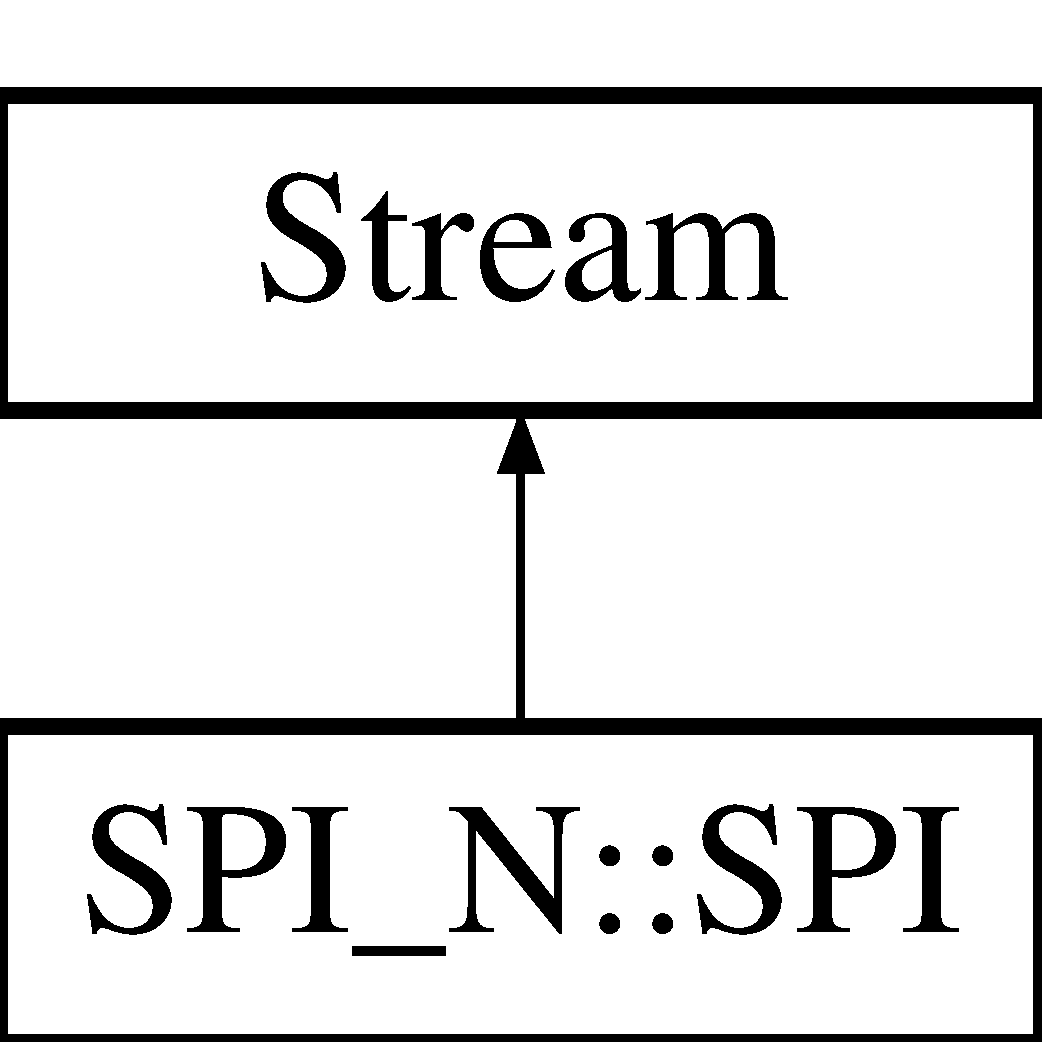
\includegraphics[height=2.000000cm]{class_s_p_i___n_1_1_s_p_i}
\end{center}
\end{figure}
\subsection*{Public Member Functions}
\begin{DoxyCompactItemize}
\item 
\hyperlink{class_s_p_i___n_1_1_s_p_i_ab486ba0f0d9ec880520e568762cc6c7d}{S\-P\-I} (const \hyperlink{class_s_p_i___n_1_1_s_p_i}{S\-P\-I} \&)=delete
\item 
\hypertarget{class_s_p_i___n_1_1_s_p_i_ad04a79c8e9139545a96af71245ce8d18}{void {\bfseries Set\-Device} (\hyperlink{struct_s_p_i___n_1_1_p_i_n}{P\-I\-N} \&pin)}\label{class_s_p_i___n_1_1_s_p_i_ad04a79c8e9139545a96af71245ce8d18}

\item 
void \hyperlink{class_s_p_i___n_1_1_s_p_i_aabc66612d396c2b70e5cbdba405dbfe5}{operator=} (const \hyperlink{class_s_p_i___n_1_1_s_p_i}{S\-P\-I} \&)=delete
\item 
void \hyperlink{class_s_p_i___n_1_1_s_p_i_a716a42a09541bb28a90a501ff54a459a}{Intiialize} (\hyperlink{struct_s_p_i___n_1_1_p_i_n}{P\-I\-N} $\ast$$\ast$pins, uint8\-\_\-t number\-\_\-of\-\_\-pins, bool clock\-\_\-polarity\-\_\-falling, bool clock\-\_\-phase\-\_\-trailing)
\item 
void \hyperlink{class_s_p_i___n_1_1_s_p_i_a3e2e2a7f02ffa5003548a1b9d820ce9a}{Write} (uint8\-\_\-t $\ast$string, uint16\-\_\-t size)
\item 
void \hyperlink{class_s_p_i___n_1_1_s_p_i_a542dc8e88203de7040ce9926d06b9463}{Write\-Byte} (uint8\-\_\-t byte, bool wait)
\item 
void \hyperlink{class_s_p_i___n_1_1_s_p_i_a05bcca2e033422b2e6ad570320d03fcb}{Write\-Byte\-And\-Throw\-Away\-Data} (uint8\-\_\-t byte, bool wait)
\item 
bool \hyperlink{class_s_p_i___n_1_1_s_p_i_a57ee9af74ec6a2d37001674f37f46344}{Read\-Byte} (uint8\-\_\-t \&data)
\item 
void \hyperlink{class_s_p_i___n_1_1_s_p_i_a6daa4720c8710e177f71ac318b96a3f8}{Reset\-S\-S\-Pin} ()
\end{DoxyCompactItemize}
\subsection*{Static Public Member Functions}
\begin{DoxyCompactItemize}
\item 
static \hyperlink{class_s_p_i___n_1_1_s_p_i}{S\-P\-I} \& \hyperlink{class_s_p_i___n_1_1_s_p_i_abc266ff9d817b8d4437d1da47fe8e7ae}{Get\-Instance} ()
\end{DoxyCompactItemize}
\subsection*{Private Member Functions}
\begin{DoxyCompactItemize}
\item 
\hyperlink{class_s_p_i___n_1_1_s_p_i_a8fec1a6e642a5758acf974b92e28a9e6}{S\-P\-I} ()
\item 
void \hyperlink{class_s_p_i___n_1_1_s_p_i_af973a5b4a970c3c01430037d578151ef}{Initialize\-Transmission} ()
\item 
void \hyperlink{class_s_p_i___n_1_1_s_p_i_a5f2091bd02e8adbe6814b12fb6e2057f}{Read\-And\-Insert\-Into\-Input\-Buffer} ()
\end{DoxyCompactItemize}
\subsection*{Private Attributes}
\begin{DoxyCompactItemize}
\item 
bool \hyperlink{class_s_p_i___n_1_1_s_p_i_aff61d4bfc6a6e0088c3653898b1e91b8}{ongoing\-\_\-transmission}
\item 
\hyperlink{struct_s_p_i___n_1_1_p_i_n}{P\-I\-N} \hyperlink{class_s_p_i___n_1_1_s_p_i_ac016c4eaed2db3f8b5523bf0d472ddd2}{current\-\_\-pin}
\item 
bool \hyperlink{class_s_p_i___n_1_1_s_p_i_a7b2d300478662920e6911cea751e1094}{throw\-\_\-away\-\_\-data}
\end{DoxyCompactItemize}
\subsection*{Friends}
\begin{DoxyCompactItemize}
\item 
void \hyperlink{class_s_p_i___n_1_1_s_p_i_a96543550133e0b0c6ae83faad5c0d68d}{S\-P\-I\-\_\-\-S\-T\-C\-\_\-vect} ()
\end{DoxyCompactItemize}


\subsection{Detailed Description}
This class is an \hyperlink{class_s_p_i___n_1_1_s_p_i}{S\-P\-I} driver which uses the 

\subsection{Constructor \& Destructor Documentation}
\hypertarget{class_s_p_i___n_1_1_s_p_i_ab486ba0f0d9ec880520e568762cc6c7d}{\index{S\-P\-I\-\_\-\-N\-::\-S\-P\-I@{S\-P\-I\-\_\-\-N\-::\-S\-P\-I}!S\-P\-I@{S\-P\-I}}
\index{S\-P\-I@{S\-P\-I}!SPI_N::SPI@{S\-P\-I\-\_\-\-N\-::\-S\-P\-I}}
\subsubsection[{S\-P\-I}]{\setlength{\rightskip}{0pt plus 5cm}S\-P\-I\-\_\-\-N\-::\-S\-P\-I\-::\-S\-P\-I (
\begin{DoxyParamCaption}
\item[{const {\bf S\-P\-I} \&}]{}
\end{DoxyParamCaption}
)\hspace{0.3cm}{\ttfamily [delete]}}}\label{class_s_p_i___n_1_1_s_p_i_ab486ba0f0d9ec880520e568762cc6c7d}
Because of singleton -\/ makes sure its not copied etc. \hypertarget{class_s_p_i___n_1_1_s_p_i_a8fec1a6e642a5758acf974b92e28a9e6}{\index{S\-P\-I\-\_\-\-N\-::\-S\-P\-I@{S\-P\-I\-\_\-\-N\-::\-S\-P\-I}!S\-P\-I@{S\-P\-I}}
\index{S\-P\-I@{S\-P\-I}!SPI_N::SPI@{S\-P\-I\-\_\-\-N\-::\-S\-P\-I}}
\subsubsection[{S\-P\-I}]{\setlength{\rightskip}{0pt plus 5cm}S\-P\-I\-\_\-\-N\-::\-S\-P\-I\-::\-S\-P\-I (
\begin{DoxyParamCaption}
{}
\end{DoxyParamCaption}
)\hspace{0.3cm}{\ttfamily [private]}}}\label{class_s_p_i___n_1_1_s_p_i_a8fec1a6e642a5758acf974b92e28a9e6}
Initializer for \hyperlink{class_s_p_i___n_1_1_s_p_i}{S\-P\-I}. Not used because of singleton 

\subsection{Member Function Documentation}
\hypertarget{class_s_p_i___n_1_1_s_p_i_abc266ff9d817b8d4437d1da47fe8e7ae}{\index{S\-P\-I\-\_\-\-N\-::\-S\-P\-I@{S\-P\-I\-\_\-\-N\-::\-S\-P\-I}!Get\-Instance@{Get\-Instance}}
\index{Get\-Instance@{Get\-Instance}!SPI_N::SPI@{S\-P\-I\-\_\-\-N\-::\-S\-P\-I}}
\subsubsection[{Get\-Instance}]{\setlength{\rightskip}{0pt plus 5cm}static {\bf S\-P\-I}\& S\-P\-I\-\_\-\-N\-::\-S\-P\-I\-::\-Get\-Instance (
\begin{DoxyParamCaption}
{}
\end{DoxyParamCaption}
)\hspace{0.3cm}{\ttfamily [inline]}, {\ttfamily [static]}}}\label{class_s_p_i___n_1_1_s_p_i_abc266ff9d817b8d4437d1da47fe8e7ae}
A Singleton implementation of this class \hypertarget{class_s_p_i___n_1_1_s_p_i_af973a5b4a970c3c01430037d578151ef}{\index{S\-P\-I\-\_\-\-N\-::\-S\-P\-I@{S\-P\-I\-\_\-\-N\-::\-S\-P\-I}!Initialize\-Transmission@{Initialize\-Transmission}}
\index{Initialize\-Transmission@{Initialize\-Transmission}!SPI_N::SPI@{S\-P\-I\-\_\-\-N\-::\-S\-P\-I}}
\subsubsection[{Initialize\-Transmission}]{\setlength{\rightskip}{0pt plus 5cm}void S\-P\-I\-\_\-\-N\-::\-S\-P\-I\-::\-Initialize\-Transmission (
\begin{DoxyParamCaption}
{}
\end{DoxyParamCaption}
)\hspace{0.3cm}{\ttfamily [private]}}}\label{class_s_p_i___n_1_1_s_p_i_af973a5b4a970c3c01430037d578151ef}
Send the data in the output buffer onto the \hyperlink{class_s_p_i___n_1_1_s_p_i}{S\-P\-I}. \hypertarget{class_s_p_i___n_1_1_s_p_i_a716a42a09541bb28a90a501ff54a459a}{\index{S\-P\-I\-\_\-\-N\-::\-S\-P\-I@{S\-P\-I\-\_\-\-N\-::\-S\-P\-I}!Intiialize@{Intiialize}}
\index{Intiialize@{Intiialize}!SPI_N::SPI@{S\-P\-I\-\_\-\-N\-::\-S\-P\-I}}
\subsubsection[{Intiialize}]{\setlength{\rightskip}{0pt plus 5cm}void S\-P\-I\-\_\-\-N\-::\-S\-P\-I\-::\-Intiialize (
\begin{DoxyParamCaption}
\item[{{\bf P\-I\-N} $\ast$$\ast$}]{pins, }
\item[{uint8\-\_\-t}]{number\-\_\-of\-\_\-pins, }
\item[{bool}]{clock\-\_\-polarity\-\_\-falling = {\ttfamily 0}, }
\item[{bool}]{clock\-\_\-phase\-\_\-trailing = {\ttfamily 0}}
\end{DoxyParamCaption}
)}}\label{class_s_p_i___n_1_1_s_p_i_a716a42a09541bb28a90a501ff54a459a}
Initializes the I\-S\-P. 
\begin{DoxyParams}{Parameters}
{\em pins} & An array with \hyperlink{struct_s_p_i___n_1_1_p_i_n}{P\-I\-N} structs, where each struct is a pin that is used by the \hyperlink{class_s_p_i___n_1_1_s_p_i}{S\-P\-I} \\
\hline
{\em number\-\_\-of\-\_\-pins} & Number of \hyperlink{struct_s_p_i___n_1_1_p_i_n}{P\-I\-N} structs in the pins array \\
\hline
{\em clock\-\_\-polarity\-\_\-falling} & If enabled, S\-C\-K is high when idle. Defaults to disabled (S\-C\-K low when idle) \\
\hline
{\em clock\-\_\-phase\-\_\-trailing} & If enabled, samples on the trailing edge of S\-C\-K\-: Defaults to disabled (sample on the leading edge) \\
\hline
\end{DoxyParams}
\hypertarget{class_s_p_i___n_1_1_s_p_i_aabc66612d396c2b70e5cbdba405dbfe5}{\index{S\-P\-I\-\_\-\-N\-::\-S\-P\-I@{S\-P\-I\-\_\-\-N\-::\-S\-P\-I}!operator=@{operator=}}
\index{operator=@{operator=}!SPI_N::SPI@{S\-P\-I\-\_\-\-N\-::\-S\-P\-I}}
\subsubsection[{operator=}]{\setlength{\rightskip}{0pt plus 5cm}void S\-P\-I\-\_\-\-N\-::\-S\-P\-I\-::operator= (
\begin{DoxyParamCaption}
\item[{const {\bf S\-P\-I} \&}]{}
\end{DoxyParamCaption}
)\hspace{0.3cm}{\ttfamily [delete]}}}\label{class_s_p_i___n_1_1_s_p_i_aabc66612d396c2b70e5cbdba405dbfe5}
Because of singleton -\/ makes sure its not copied etc. \hypertarget{class_s_p_i___n_1_1_s_p_i_a5f2091bd02e8adbe6814b12fb6e2057f}{\index{S\-P\-I\-\_\-\-N\-::\-S\-P\-I@{S\-P\-I\-\_\-\-N\-::\-S\-P\-I}!Read\-And\-Insert\-Into\-Input\-Buffer@{Read\-And\-Insert\-Into\-Input\-Buffer}}
\index{Read\-And\-Insert\-Into\-Input\-Buffer@{Read\-And\-Insert\-Into\-Input\-Buffer}!SPI_N::SPI@{S\-P\-I\-\_\-\-N\-::\-S\-P\-I}}
\subsubsection[{Read\-And\-Insert\-Into\-Input\-Buffer}]{\setlength{\rightskip}{0pt plus 5cm}void S\-P\-I\-\_\-\-N\-::\-S\-P\-I\-::\-Read\-And\-Insert\-Into\-Input\-Buffer (
\begin{DoxyParamCaption}
{}
\end{DoxyParamCaption}
)\hspace{0.3cm}{\ttfamily [private]}}}\label{class_s_p_i___n_1_1_s_p_i_a5f2091bd02e8adbe6814b12fb6e2057f}
Reads the data from the \hyperlink{class_s_p_i___n_1_1_s_p_i}{S\-P\-I} and puts it inot the input buffer \hypertarget{class_s_p_i___n_1_1_s_p_i_a57ee9af74ec6a2d37001674f37f46344}{\index{S\-P\-I\-\_\-\-N\-::\-S\-P\-I@{S\-P\-I\-\_\-\-N\-::\-S\-P\-I}!Read\-Byte@{Read\-Byte}}
\index{Read\-Byte@{Read\-Byte}!SPI_N::SPI@{S\-P\-I\-\_\-\-N\-::\-S\-P\-I}}
\subsubsection[{Read\-Byte}]{\setlength{\rightskip}{0pt plus 5cm}bool S\-P\-I\-\_\-\-N\-::\-S\-P\-I\-::\-Read\-Byte (
\begin{DoxyParamCaption}
\item[{uint8\-\_\-t \&}]{data}
\end{DoxyParamCaption}
)\hspace{0.3cm}{\ttfamily [virtual]}}}\label{class_s_p_i___n_1_1_s_p_i_a57ee9af74ec6a2d37001674f37f46344}
Reads a byte from the input stream 
\begin{DoxyParams}{Parameters}
{\em data} & Byte to insert the byte into \\
\hline
\end{DoxyParams}


Reimplemented from \hyperlink{class_stream_a6db4180f5834073f992608b856bddca2}{Stream}.

\hypertarget{class_s_p_i___n_1_1_s_p_i_a6daa4720c8710e177f71ac318b96a3f8}{\index{S\-P\-I\-\_\-\-N\-::\-S\-P\-I@{S\-P\-I\-\_\-\-N\-::\-S\-P\-I}!Reset\-S\-S\-Pin@{Reset\-S\-S\-Pin}}
\index{Reset\-S\-S\-Pin@{Reset\-S\-S\-Pin}!SPI_N::SPI@{S\-P\-I\-\_\-\-N\-::\-S\-P\-I}}
\subsubsection[{Reset\-S\-S\-Pin}]{\setlength{\rightskip}{0pt plus 5cm}void S\-P\-I\-\_\-\-N\-::\-S\-P\-I\-::\-Reset\-S\-S\-Pin (
\begin{DoxyParamCaption}
{}
\end{DoxyParamCaption}
)}}\label{class_s_p_i___n_1_1_s_p_i_a6daa4720c8710e177f71ac318b96a3f8}
Resets the S\-S pin. That is, if the S\-S pin is high, put it low and then high again. If it is low, put it high and then low again \hypertarget{class_s_p_i___n_1_1_s_p_i_a3e2e2a7f02ffa5003548a1b9d820ce9a}{\index{S\-P\-I\-\_\-\-N\-::\-S\-P\-I@{S\-P\-I\-\_\-\-N\-::\-S\-P\-I}!Write@{Write}}
\index{Write@{Write}!SPI_N::SPI@{S\-P\-I\-\_\-\-N\-::\-S\-P\-I}}
\subsubsection[{Write}]{\setlength{\rightskip}{0pt plus 5cm}void S\-P\-I\-\_\-\-N\-::\-S\-P\-I\-::\-Write (
\begin{DoxyParamCaption}
\item[{uint8\-\_\-t $\ast$}]{string, }
\item[{uint16\-\_\-t}]{size}
\end{DoxyParamCaption}
)\hspace{0.3cm}{\ttfamily [virtual]}}}\label{class_s_p_i___n_1_1_s_p_i_a3e2e2a7f02ffa5003548a1b9d820ce9a}
Write the inserted string to output (i.\-e. write to \hyperlink{class_s_p_i___n_1_1_s_p_i}{S\-P\-I} selected by Set\-Device) 
\begin{DoxyParams}{Parameters}
{\em string} & The \char`\"{}data string\char`\"{} that shall be written to the output \\
\hline
{\em size} & the size of the data string \\
\hline
\end{DoxyParams}


Reimplemented from \hyperlink{class_stream_a508be3423e4d99ab2757275fb723002a}{Stream}.

\hypertarget{class_s_p_i___n_1_1_s_p_i_a542dc8e88203de7040ce9926d06b9463}{\index{S\-P\-I\-\_\-\-N\-::\-S\-P\-I@{S\-P\-I\-\_\-\-N\-::\-S\-P\-I}!Write\-Byte@{Write\-Byte}}
\index{Write\-Byte@{Write\-Byte}!SPI_N::SPI@{S\-P\-I\-\_\-\-N\-::\-S\-P\-I}}
\subsubsection[{Write\-Byte}]{\setlength{\rightskip}{0pt plus 5cm}void S\-P\-I\-\_\-\-N\-::\-S\-P\-I\-::\-Write\-Byte (
\begin{DoxyParamCaption}
\item[{uint8\-\_\-t}]{byte, }
\item[{bool}]{wait}
\end{DoxyParamCaption}
)}}\label{class_s_p_i___n_1_1_s_p_i_a542dc8e88203de7040ce9926d06b9463}
Writes a byte to the output stream. Puts the returned data into the input stream 
\begin{DoxyParams}{Parameters}
{\em byte} & The byte to be sent \\
\hline
{\em wait} & If set, the \hyperlink{class_s_p_i___n_1_1_s_p_i}{S\-P\-I} driver will not start the transmission of the output buffer \\
\hline
\end{DoxyParams}
\hypertarget{class_s_p_i___n_1_1_s_p_i_a05bcca2e033422b2e6ad570320d03fcb}{\index{S\-P\-I\-\_\-\-N\-::\-S\-P\-I@{S\-P\-I\-\_\-\-N\-::\-S\-P\-I}!Write\-Byte\-And\-Throw\-Away\-Data@{Write\-Byte\-And\-Throw\-Away\-Data}}
\index{Write\-Byte\-And\-Throw\-Away\-Data@{Write\-Byte\-And\-Throw\-Away\-Data}!SPI_N::SPI@{S\-P\-I\-\_\-\-N\-::\-S\-P\-I}}
\subsubsection[{Write\-Byte\-And\-Throw\-Away\-Data}]{\setlength{\rightskip}{0pt plus 5cm}void S\-P\-I\-\_\-\-N\-::\-S\-P\-I\-::\-Write\-Byte\-And\-Throw\-Away\-Data (
\begin{DoxyParamCaption}
\item[{uint8\-\_\-t}]{byte, }
\item[{bool}]{wait}
\end{DoxyParamCaption}
)}}\label{class_s_p_i___n_1_1_s_p_i_a05bcca2e033422b2e6ad570320d03fcb}
Writes a byte to the output stream. Throws away the returned data 
\begin{DoxyParams}{Parameters}
{\em byte} & The byte to be sent \\
\hline
{\em wait} & If set, the \hyperlink{class_s_p_i___n_1_1_s_p_i}{S\-P\-I} driver will not start the transmission of the output buffer \\
\hline
\end{DoxyParams}


\subsection{Friends And Related Function Documentation}
\hypertarget{class_s_p_i___n_1_1_s_p_i_a96543550133e0b0c6ae83faad5c0d68d}{\index{S\-P\-I\-\_\-\-N\-::\-S\-P\-I@{S\-P\-I\-\_\-\-N\-::\-S\-P\-I}!S\-P\-I\-\_\-\-S\-T\-C\-\_\-vect@{S\-P\-I\-\_\-\-S\-T\-C\-\_\-vect}}
\index{S\-P\-I\-\_\-\-S\-T\-C\-\_\-vect@{S\-P\-I\-\_\-\-S\-T\-C\-\_\-vect}!SPI_N::SPI@{S\-P\-I\-\_\-\-N\-::\-S\-P\-I}}
\subsubsection[{S\-P\-I\-\_\-\-S\-T\-C\-\_\-vect}]{\setlength{\rightskip}{0pt plus 5cm}void S\-P\-I\-\_\-\-S\-T\-C\-\_\-vect (
\begin{DoxyParamCaption}
{}
\end{DoxyParamCaption}
)\hspace{0.3cm}{\ttfamily [friend]}}}\label{class_s_p_i___n_1_1_s_p_i_a96543550133e0b0c6ae83faad5c0d68d}
The interrupt vector for when a transmission is complete. 

\subsection{Member Data Documentation}
\hypertarget{class_s_p_i___n_1_1_s_p_i_ac016c4eaed2db3f8b5523bf0d472ddd2}{\index{S\-P\-I\-\_\-\-N\-::\-S\-P\-I@{S\-P\-I\-\_\-\-N\-::\-S\-P\-I}!current\-\_\-pin@{current\-\_\-pin}}
\index{current\-\_\-pin@{current\-\_\-pin}!SPI_N::SPI@{S\-P\-I\-\_\-\-N\-::\-S\-P\-I}}
\subsubsection[{current\-\_\-pin}]{\setlength{\rightskip}{0pt plus 5cm}{\bf P\-I\-N} S\-P\-I\-\_\-\-N\-::\-S\-P\-I\-::current\-\_\-pin\hspace{0.3cm}{\ttfamily [private]}}}\label{class_s_p_i___n_1_1_s_p_i_ac016c4eaed2db3f8b5523bf0d472ddd2}
A struct of the type \hyperlink{struct_s_p_i___n_1_1_p_i_n}{P\-I\-N} which indicates which pin is currently selected. \hypertarget{class_s_p_i___n_1_1_s_p_i_aff61d4bfc6a6e0088c3653898b1e91b8}{\index{S\-P\-I\-\_\-\-N\-::\-S\-P\-I@{S\-P\-I\-\_\-\-N\-::\-S\-P\-I}!ongoing\-\_\-transmission@{ongoing\-\_\-transmission}}
\index{ongoing\-\_\-transmission@{ongoing\-\_\-transmission}!SPI_N::SPI@{S\-P\-I\-\_\-\-N\-::\-S\-P\-I}}
\subsubsection[{ongoing\-\_\-transmission}]{\setlength{\rightskip}{0pt plus 5cm}bool S\-P\-I\-\_\-\-N\-::\-S\-P\-I\-::ongoing\-\_\-transmission\hspace{0.3cm}{\ttfamily [private]}}}\label{class_s_p_i___n_1_1_s_p_i_aff61d4bfc6a6e0088c3653898b1e91b8}
A bool indicating wether or not an outgoing transmission is ongoing \hypertarget{class_s_p_i___n_1_1_s_p_i_a7b2d300478662920e6911cea751e1094}{\index{S\-P\-I\-\_\-\-N\-::\-S\-P\-I@{S\-P\-I\-\_\-\-N\-::\-S\-P\-I}!throw\-\_\-away\-\_\-data@{throw\-\_\-away\-\_\-data}}
\index{throw\-\_\-away\-\_\-data@{throw\-\_\-away\-\_\-data}!SPI_N::SPI@{S\-P\-I\-\_\-\-N\-::\-S\-P\-I}}
\subsubsection[{throw\-\_\-away\-\_\-data}]{\setlength{\rightskip}{0pt plus 5cm}bool S\-P\-I\-\_\-\-N\-::\-S\-P\-I\-::throw\-\_\-away\-\_\-data\hspace{0.3cm}{\ttfamily [private]}}}\label{class_s_p_i___n_1_1_s_p_i_a7b2d300478662920e6911cea751e1094}
A flag indicating whether or not to keep the next recieved byte 

The documentation for this class was generated from the following files\-:\begin{DoxyCompactItemize}
\item 
lib/spi/\hyperlink{spi_8h}{spi.\-h}\item 
lib/spi/spi.\-cpp\end{DoxyCompactItemize}

\hypertarget{class_stream}{\section{Stream Class Reference}
\label{class_stream}\index{Stream@{Stream}}
}
Inheritance diagram for Stream\-:\begin{figure}[H]
\begin{center}
\leavevmode
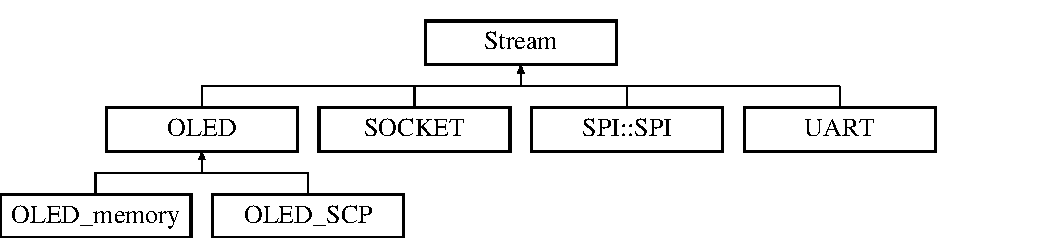
\includegraphics[height=2.000000cm]{class_stream}
\end{center}
\end{figure}
\subsection*{Public Member Functions}
\begin{DoxyCompactItemize}
\item 
\hyperlink{class_stream_afd83bbd749c467ad3dd85e1b80170c9b}{Stream} (uint8\-\_\-t $\ast$\hyperlink{class_stream_aaa6b266a85844345faee432d0267c6ec}{input\-\_\-stream}, uint16\-\_\-t \hyperlink{class_stream_a8a754b0acc9552d1b78de92b2476f4cb}{input\-\_\-stream\-\_\-size}, uint8\-\_\-t $\ast$\hyperlink{class_stream_ab2d136f405b24e5eb2a6058b24fabfa3}{output\-\_\-stream}, uint16\-\_\-t \hyperlink{class_stream_a3a171d646ab70eeb9c034aecb3a72003}{output\-\_\-stream\-\_\-size})
\item 
virtual void \hyperlink{class_stream_a508be3423e4d99ab2757275fb723002a}{Write} (uint8\-\_\-t $\ast$string, uint16\-\_\-t size)
\item 
virtual void \hyperlink{class_stream_a4f3ec0f7a24ddcfd054566feb614afba}{Read} (uint8\-\_\-t $\ast$string, uint16\-\_\-t size)
\item 
virtual uint8\-\_\-t \hyperlink{class_stream_aeb3f1b3d55f4b502c02d73ce4de42714}{Read\-Byte} ()
\item 
virtual void \hyperlink{class_stream_aeaed767b3a8d946c6f81465fa83ff17f}{Write\-Byte} (uint8\-\_\-t byte)
\item 
virtual uint8\-\_\-t \hyperlink{class_stream_a6a16ddb03d3360cef4daf4d38245091d}{Get\-Available\-Write\-Bytes} ()
\item 
virtual uint8\-\_\-t \hyperlink{class_stream_a71cec6c46f3d50cc3ab420e93ae434e1}{Get\-Available\-Read\-Bytes} ()
\item 
virtual bool \hyperlink{class_stream_a088c4e68d568acfad715c56f408fe9f8}{Check\-Input\-Overflow\-Flag} ()
\item 
virtual bool \hyperlink{class_stream_aee6c201819b874c5934a270592d9d311}{Check\-Output\-Overflow\-Flag} ()
\end{DoxyCompactItemize}
\subsection*{Protected Member Functions}
\begin{DoxyCompactItemize}
\item 
virtual void \hyperlink{class_stream_add5927208d603b08341f8972652d9c44}{Read\-From\-Buffer} (uint8\-\_\-t $\ast$buffer, uint16\-\_\-t \&start\-\_\-index, uint16\-\_\-t \&stop\-\_\-index, uint16\-\_\-t \&buffer\-\_\-size, uint8\-\_\-t $\ast$string, uint16\-\_\-t \&string\-\_\-size)
\item 
virtual void \hyperlink{class_stream_a456d59b1944143a8e4a977b8861d42ea}{Write\-To\-Buffer} (uint8\-\_\-t $\ast$buffer, uint16\-\_\-t \&start\-\_\-index, uint16\-\_\-t \&stop\-\_\-index, uint16\-\_\-t \&buffer\-\_\-size, bool \&overflow\-\_\-flag, uint8\-\_\-t $\ast$string, uint16\-\_\-t \&string\-\_\-size)
\item 
virtual uint8\-\_\-t \hyperlink{class_stream_a6c49bb8565d238e13c3ca3e9eddcf38e}{Read\-Byte\-From\-Buffer} (uint8\-\_\-t $\ast$buffer, uint16\-\_\-t \&start\-\_\-index, uint16\-\_\-t \&stop\-\_\-index, uint16\-\_\-t \&buffer\-\_\-size)
\item 
virtual void \hyperlink{class_stream_a129f3c3e763ceab692bdde38fdc89402}{Write\-Byte\-To\-Buffer} (uint8\-\_\-t $\ast$buffer, uint16\-\_\-t \&start\-\_\-index, uint16\-\_\-t \&stop\-\_\-index, uint16\-\_\-t \&buffer\-\_\-size, bool \&overflow\-\_\-flag, uint8\-\_\-t \&byte)
\item 
virtual void \hyperlink{class_stream_a70108ab0e811c6cab2636bf7afeb5e14}{Write\-Byte\-To\-Input\-Stream} (uint8\-\_\-t byte)
\item 
virtual uint8\-\_\-t \hyperlink{class_stream_a712a8e0c6659799b1bb2999b53bd983d}{Read\-Byte\-From\-Output\-Stream} ()
\item 
virtual void \hyperlink{class_stream_aa2f020721d273ce821ccf626e5eb773c}{Write\-To\-Input\-Stream} (uint8\-\_\-t $\ast$string, uint16\-\_\-t size)
\item 
virtual void \hyperlink{class_stream_adce437b86a098710237ac7dcccd5508d}{Read\-From\-Output\-Stream} (uint8\-\_\-t $\ast$string, uint16\-\_\-t size)
\item 
virtual uint16\-\_\-t \hyperlink{class_stream_a8abdeaae6339d9873842a951843cb386}{Calculate\-Length} (uint16\-\_\-t \&start\-\_\-index, uint16\-\_\-t \&stop\-\_\-index, uint16\-\_\-t \&buffer\-\_\-size)
\item 
virtual uint16\-\_\-t \hyperlink{class_stream_ac9d4705ce8fe5c9ac473939fcac423f6}{Get\-Input\-Stream\-Length} ()
\item 
virtual uint16\-\_\-t \hyperlink{class_stream_a6378bb812d0b77890926d1c724140146}{Get\-Output\-Stream\-Length} ()
\end{DoxyCompactItemize}
\subsection*{Protected Attributes}
\begin{DoxyCompactItemize}
\item 
uint8\-\_\-t $\ast$ \hyperlink{class_stream_aaa6b266a85844345faee432d0267c6ec}{input\-\_\-stream} = nullptr
\item 
uint8\-\_\-t $\ast$ \hyperlink{class_stream_ab2d136f405b24e5eb2a6058b24fabfa3}{output\-\_\-stream} = nullptr
\item 
uint16\-\_\-t \hyperlink{class_stream_ade2d5afb993214626e7c7d66cb76cd46}{input\-\_\-stream\-\_\-start\-\_\-index} = 0
\item 
uint16\-\_\-t \hyperlink{class_stream_a7406f5db92c18f0a6d7dcc924a6122cc}{output\-\_\-stream\-\_\-start\-\_\-index} = 0
\item 
uint16\-\_\-t \hyperlink{class_stream_a52cf2f675dd7ec342615e82cc29513de}{input\-\_\-stream\-\_\-stop\-\_\-index} = 0
\item 
uint16\-\_\-t \hyperlink{class_stream_ac3b2282b5977151124aa77c2d4e411ec}{output\-\_\-stream\-\_\-stop\-\_\-index} = 0
\item 
uint16\-\_\-t \hyperlink{class_stream_a3a171d646ab70eeb9c034aecb3a72003}{output\-\_\-stream\-\_\-size} = 0
\item 
uint16\-\_\-t \hyperlink{class_stream_a8a754b0acc9552d1b78de92b2476f4cb}{input\-\_\-stream\-\_\-size} = 0
\item 
bool \hyperlink{class_stream_aeffd88d8ca71bf0d084ded2a251e3a57}{input\-\_\-stream\-\_\-overflowed} = false
\item 
bool \hyperlink{class_stream_a91eb40b21c46bd57b61811a890ac047a}{output\-\_\-stream\-\_\-overflowed} = false
\end{DoxyCompactItemize}


\subsection{Constructor \& Destructor Documentation}
\hypertarget{class_stream_afd83bbd749c467ad3dd85e1b80170c9b}{\index{Stream@{Stream}!Stream@{Stream}}
\index{Stream@{Stream}!Stream@{Stream}}
\subsubsection[{Stream}]{\setlength{\rightskip}{0pt plus 5cm}Stream\-::\-Stream (
\begin{DoxyParamCaption}
\item[{uint8\-\_\-t $\ast$}]{input\-\_\-stream, }
\item[{uint16\-\_\-t}]{input\-\_\-stream\-\_\-size, }
\item[{uint8\-\_\-t $\ast$}]{output\-\_\-stream, }
\item[{uint16\-\_\-t}]{output\-\_\-stream\-\_\-size}
\end{DoxyParamCaption}
)\hspace{0.3cm}{\ttfamily [inline]}}}\label{class_stream_afd83bbd749c467ad3dd85e1b80170c9b}
The constructor. Needed to initialize stream sizes 
\begin{DoxyParams}{Parameters}
{\em input\-\_\-stream\-\_\-size} & The size of the input ring buffer. \\
\hline
{\em output\-\_\-stream\-\_\-size} & The size of the output ring buffer. \\
\hline
\end{DoxyParams}


\subsection{Member Function Documentation}
\hypertarget{class_stream_a8abdeaae6339d9873842a951843cb386}{\index{Stream@{Stream}!Calculate\-Length@{Calculate\-Length}}
\index{Calculate\-Length@{Calculate\-Length}!Stream@{Stream}}
\subsubsection[{Calculate\-Length}]{\setlength{\rightskip}{0pt plus 5cm}uint16\-\_\-t Stream\-::\-Calculate\-Length (
\begin{DoxyParamCaption}
\item[{uint16\-\_\-t \&}]{start\-\_\-index, }
\item[{uint16\-\_\-t \&}]{stop\-\_\-index, }
\item[{uint16\-\_\-t \&}]{buffer\-\_\-size}
\end{DoxyParamCaption}
)\hspace{0.3cm}{\ttfamily [protected]}, {\ttfamily [virtual]}}}\label{class_stream_a8abdeaae6339d9873842a951843cb386}
Calculates the length of the readable part of the buffer 
\begin{DoxyParams}{Parameters}
{\em start\-\_\-index} & The start index of the buffer \\
\hline
{\em stop\-\_\-index} & The stop index of the buffer \\
\hline
\end{DoxyParams}
\begin{DoxyReturn}{Returns}
Length of valid data 
\end{DoxyReturn}
\hypertarget{class_stream_a088c4e68d568acfad715c56f408fe9f8}{\index{Stream@{Stream}!Check\-Input\-Overflow\-Flag@{Check\-Input\-Overflow\-Flag}}
\index{Check\-Input\-Overflow\-Flag@{Check\-Input\-Overflow\-Flag}!Stream@{Stream}}
\subsubsection[{Check\-Input\-Overflow\-Flag}]{\setlength{\rightskip}{0pt plus 5cm}bool Stream\-::\-Check\-Input\-Overflow\-Flag (
\begin{DoxyParamCaption}
{}
\end{DoxyParamCaption}
)\hspace{0.3cm}{\ttfamily [virtual]}}}\label{class_stream_a088c4e68d568acfad715c56f408fe9f8}
Checks whether or not the input overflow flag has been set. If it has, it conducts the nessesary procedures to clear out the overflow \hypertarget{class_stream_aee6c201819b874c5934a270592d9d311}{\index{Stream@{Stream}!Check\-Output\-Overflow\-Flag@{Check\-Output\-Overflow\-Flag}}
\index{Check\-Output\-Overflow\-Flag@{Check\-Output\-Overflow\-Flag}!Stream@{Stream}}
\subsubsection[{Check\-Output\-Overflow\-Flag}]{\setlength{\rightskip}{0pt plus 5cm}bool Stream\-::\-Check\-Output\-Overflow\-Flag (
\begin{DoxyParamCaption}
{}
\end{DoxyParamCaption}
)\hspace{0.3cm}{\ttfamily [virtual]}}}\label{class_stream_aee6c201819b874c5934a270592d9d311}
Checks whether or not the output overflow flag has been set. If it has, it conducts the nessesary procedures to clear out the overflow \hypertarget{class_stream_a71cec6c46f3d50cc3ab420e93ae434e1}{\index{Stream@{Stream}!Get\-Available\-Read\-Bytes@{Get\-Available\-Read\-Bytes}}
\index{Get\-Available\-Read\-Bytes@{Get\-Available\-Read\-Bytes}!Stream@{Stream}}
\subsubsection[{Get\-Available\-Read\-Bytes}]{\setlength{\rightskip}{0pt plus 5cm}uint8\-\_\-t Stream\-::\-Get\-Available\-Read\-Bytes (
\begin{DoxyParamCaption}
{}
\end{DoxyParamCaption}
)\hspace{0.3cm}{\ttfamily [virtual]}}}\label{class_stream_a71cec6c46f3d50cc3ab420e93ae434e1}
Simply returns the number of bytes available for reading (the actual data available for receiving in the buffer) \hypertarget{class_stream_a6a16ddb03d3360cef4daf4d38245091d}{\index{Stream@{Stream}!Get\-Available\-Write\-Bytes@{Get\-Available\-Write\-Bytes}}
\index{Get\-Available\-Write\-Bytes@{Get\-Available\-Write\-Bytes}!Stream@{Stream}}
\subsubsection[{Get\-Available\-Write\-Bytes}]{\setlength{\rightskip}{0pt plus 5cm}uint8\-\_\-t Stream\-::\-Get\-Available\-Write\-Bytes (
\begin{DoxyParamCaption}
{}
\end{DoxyParamCaption}
)\hspace{0.3cm}{\ttfamily [virtual]}}}\label{class_stream_a6a16ddb03d3360cef4daf4d38245091d}
Simply returns the number of bytes available in the output buffer. The output depends on the maximum bytes allocated in the implementation. \hypertarget{class_stream_ac9d4705ce8fe5c9ac473939fcac423f6}{\index{Stream@{Stream}!Get\-Input\-Stream\-Length@{Get\-Input\-Stream\-Length}}
\index{Get\-Input\-Stream\-Length@{Get\-Input\-Stream\-Length}!Stream@{Stream}}
\subsubsection[{Get\-Input\-Stream\-Length}]{\setlength{\rightskip}{0pt plus 5cm}uint16\-\_\-t Stream\-::\-Get\-Input\-Stream\-Length (
\begin{DoxyParamCaption}
{}
\end{DoxyParamCaption}
)\hspace{0.3cm}{\ttfamily [protected]}, {\ttfamily [virtual]}}}\label{class_stream_ac9d4705ce8fe5c9ac473939fcac423f6}
Calculates the length of the readable part of the buffer 
\begin{DoxyParams}{Parameters}
{\em start\-\_\-index} & The start index of the buffer \\
\hline
{\em stop\-\_\-index} & The stop index of the buffer \\
\hline
\end{DoxyParams}
\begin{DoxyReturn}{Returns}
Length of valid data 
\end{DoxyReturn}
\hypertarget{class_stream_a6378bb812d0b77890926d1c724140146}{\index{Stream@{Stream}!Get\-Output\-Stream\-Length@{Get\-Output\-Stream\-Length}}
\index{Get\-Output\-Stream\-Length@{Get\-Output\-Stream\-Length}!Stream@{Stream}}
\subsubsection[{Get\-Output\-Stream\-Length}]{\setlength{\rightskip}{0pt plus 5cm}uint16\-\_\-t Stream\-::\-Get\-Output\-Stream\-Length (
\begin{DoxyParamCaption}
{}
\end{DoxyParamCaption}
)\hspace{0.3cm}{\ttfamily [protected]}, {\ttfamily [virtual]}}}\label{class_stream_a6378bb812d0b77890926d1c724140146}
Calculates the length of the readable part of the buffer \begin{DoxyReturn}{Returns}
Length of valid data 
\end{DoxyReturn}
\hypertarget{class_stream_a4f3ec0f7a24ddcfd054566feb614afba}{\index{Stream@{Stream}!Read@{Read}}
\index{Read@{Read}!Stream@{Stream}}
\subsubsection[{Read}]{\setlength{\rightskip}{0pt plus 5cm}void Stream\-::\-Read (
\begin{DoxyParamCaption}
\item[{uint8\-\_\-t $\ast$}]{string, }
\item[{uint16\-\_\-t}]{size}
\end{DoxyParamCaption}
)\hspace{0.3cm}{\ttfamily [virtual]}}}\label{class_stream_a4f3ec0f7a24ddcfd054566feb614afba}
Reads data from the input stream and stores in the specified data. 
\begin{DoxyParams}{Parameters}
{\em string} & Where the data should be stored \\
\hline
{\em size} & Size of the data \\
\hline
\end{DoxyParams}
\hypertarget{class_stream_aeb3f1b3d55f4b502c02d73ce4de42714}{\index{Stream@{Stream}!Read\-Byte@{Read\-Byte}}
\index{Read\-Byte@{Read\-Byte}!Stream@{Stream}}
\subsubsection[{Read\-Byte}]{\setlength{\rightskip}{0pt plus 5cm}uint8\-\_\-t Stream\-::\-Read\-Byte (
\begin{DoxyParamCaption}
{}
\end{DoxyParamCaption}
)\hspace{0.3cm}{\ttfamily [virtual]}}}\label{class_stream_aeb3f1b3d55f4b502c02d73ce4de42714}
Reads one byte from the input stream \hypertarget{class_stream_a6c49bb8565d238e13c3ca3e9eddcf38e}{\index{Stream@{Stream}!Read\-Byte\-From\-Buffer@{Read\-Byte\-From\-Buffer}}
\index{Read\-Byte\-From\-Buffer@{Read\-Byte\-From\-Buffer}!Stream@{Stream}}
\subsubsection[{Read\-Byte\-From\-Buffer}]{\setlength{\rightskip}{0pt plus 5cm}uint8\-\_\-t Stream\-::\-Read\-Byte\-From\-Buffer (
\begin{DoxyParamCaption}
\item[{uint8\-\_\-t $\ast$}]{buffer, }
\item[{uint16\-\_\-t \&}]{start\-\_\-index, }
\item[{uint16\-\_\-t \&}]{stop\-\_\-index, }
\item[{uint16\-\_\-t \&}]{buffer\-\_\-size}
\end{DoxyParamCaption}
)\hspace{0.3cm}{\ttfamily [protected]}, {\ttfamily [virtual]}}}\label{class_stream_a6c49bb8565d238e13c3ca3e9eddcf38e}
Reads a byte from the given buffer 
\begin{DoxyParams}{Parameters}
{\em buffer} & The buffer to read from \\
\hline
{\em start\-\_\-index} & The first valid bit of the buffer \\
\hline
{\em stop\-\_\-index} & The last valid bit of the buffer \\
\hline
{\em size} & The size of the buffer \\
\hline
\end{DoxyParams}
\begin{DoxyReturn}{Returns}
The byte that was read 
\end{DoxyReturn}
\hypertarget{class_stream_a712a8e0c6659799b1bb2999b53bd983d}{\index{Stream@{Stream}!Read\-Byte\-From\-Output\-Stream@{Read\-Byte\-From\-Output\-Stream}}
\index{Read\-Byte\-From\-Output\-Stream@{Read\-Byte\-From\-Output\-Stream}!Stream@{Stream}}
\subsubsection[{Read\-Byte\-From\-Output\-Stream}]{\setlength{\rightskip}{0pt plus 5cm}uint8\-\_\-t Stream\-::\-Read\-Byte\-From\-Output\-Stream (
\begin{DoxyParamCaption}
{}
\end{DoxyParamCaption}
)\hspace{0.3cm}{\ttfamily [protected]}, {\ttfamily [virtual]}}}\label{class_stream_a712a8e0c6659799b1bb2999b53bd983d}
Reads a byte from the output stream \hypertarget{class_stream_add5927208d603b08341f8972652d9c44}{\index{Stream@{Stream}!Read\-From\-Buffer@{Read\-From\-Buffer}}
\index{Read\-From\-Buffer@{Read\-From\-Buffer}!Stream@{Stream}}
\subsubsection[{Read\-From\-Buffer}]{\setlength{\rightskip}{0pt plus 5cm}void Stream\-::\-Read\-From\-Buffer (
\begin{DoxyParamCaption}
\item[{uint8\-\_\-t $\ast$}]{buffer, }
\item[{uint16\-\_\-t \&}]{start\-\_\-index, }
\item[{uint16\-\_\-t \&}]{stop\-\_\-index, }
\item[{uint16\-\_\-t \&}]{buffer\-\_\-size, }
\item[{uint8\-\_\-t $\ast$}]{string, }
\item[{uint16\-\_\-t \&}]{string\-\_\-size}
\end{DoxyParamCaption}
)\hspace{0.3cm}{\ttfamily [protected]}, {\ttfamily [virtual]}}}\label{class_stream_add5927208d603b08341f8972652d9c44}
Reads a string from the given buffer. 
\begin{DoxyParams}{Parameters}
{\em buffer} & Buffer to read from \\
\hline
{\em start\-\_\-index} & The first valid byte of the buffer \\
\hline
{\em stop\-\_\-index} & The last valid byte of the buffer \\
\hline
{\em size} & The size of the buffer \\
\hline
{\em string} & The string to read into \\
\hline
{\em length} & The length of the string \\
\hline
\end{DoxyParams}
\hypertarget{class_stream_adce437b86a098710237ac7dcccd5508d}{\index{Stream@{Stream}!Read\-From\-Output\-Stream@{Read\-From\-Output\-Stream}}
\index{Read\-From\-Output\-Stream@{Read\-From\-Output\-Stream}!Stream@{Stream}}
\subsubsection[{Read\-From\-Output\-Stream}]{\setlength{\rightskip}{0pt plus 5cm}void Stream\-::\-Read\-From\-Output\-Stream (
\begin{DoxyParamCaption}
\item[{uint8\-\_\-t $\ast$}]{string, }
\item[{uint16\-\_\-t}]{size}
\end{DoxyParamCaption}
)\hspace{0.3cm}{\ttfamily [protected]}, {\ttfamily [virtual]}}}\label{class_stream_adce437b86a098710237ac7dcccd5508d}
Reads data from the input stream and stores in the specified data. 
\begin{DoxyParams}{Parameters}
{\em string} & Where the data should be stored \\
\hline
{\em size} & Size of the data \\
\hline
\end{DoxyParams}
\hypertarget{class_stream_a508be3423e4d99ab2757275fb723002a}{\index{Stream@{Stream}!Write@{Write}}
\index{Write@{Write}!Stream@{Stream}}
\subsubsection[{Write}]{\setlength{\rightskip}{0pt plus 5cm}void Stream\-::\-Write (
\begin{DoxyParamCaption}
\item[{uint8\-\_\-t $\ast$}]{string, }
\item[{uint16\-\_\-t}]{size}
\end{DoxyParamCaption}
)\hspace{0.3cm}{\ttfamily [virtual]}}}\label{class_stream_a508be3423e4d99ab2757275fb723002a}
Writes the specified data to the output stream. 
\begin{DoxyParams}{Parameters}
{\em string} & Input data \\
\hline
{\em size} & Size of the input data \\
\hline
\end{DoxyParams}
\hypertarget{class_stream_aeaed767b3a8d946c6f81465fa83ff17f}{\index{Stream@{Stream}!Write\-Byte@{Write\-Byte}}
\index{Write\-Byte@{Write\-Byte}!Stream@{Stream}}
\subsubsection[{Write\-Byte}]{\setlength{\rightskip}{0pt plus 5cm}void Stream\-::\-Write\-Byte (
\begin{DoxyParamCaption}
\item[{uint8\-\_\-t}]{byte}
\end{DoxyParamCaption}
)\hspace{0.3cm}{\ttfamily [virtual]}}}\label{class_stream_aeaed767b3a8d946c6f81465fa83ff17f}
Writes one byte to the output stream \hypertarget{class_stream_a129f3c3e763ceab692bdde38fdc89402}{\index{Stream@{Stream}!Write\-Byte\-To\-Buffer@{Write\-Byte\-To\-Buffer}}
\index{Write\-Byte\-To\-Buffer@{Write\-Byte\-To\-Buffer}!Stream@{Stream}}
\subsubsection[{Write\-Byte\-To\-Buffer}]{\setlength{\rightskip}{0pt plus 5cm}void Stream\-::\-Write\-Byte\-To\-Buffer (
\begin{DoxyParamCaption}
\item[{uint8\-\_\-t $\ast$}]{buffer, }
\item[{uint16\-\_\-t \&}]{start\-\_\-index, }
\item[{uint16\-\_\-t \&}]{stop\-\_\-index, }
\item[{uint16\-\_\-t \&}]{buffer\-\_\-size, }
\item[{bool \&}]{overflow\-\_\-flag, }
\item[{uint8\-\_\-t \&}]{byte}
\end{DoxyParamCaption}
)\hspace{0.3cm}{\ttfamily [protected]}, {\ttfamily [virtual]}}}\label{class_stream_a129f3c3e763ceab692bdde38fdc89402}
Writes a byte to the buffer 
\begin{DoxyParams}{Parameters}
{\em buffer} & The buffer to write to \\
\hline
{\em start\-\_\-index} & The first valid bit of the buffer \\
\hline
{\em stop\-\_\-index} & The last valid bit of the buffer \\
\hline
{\em size} & The size of the buffer \\
\hline
{\em byte} & The byte to be written \\
\hline
{\em overflow\-\_\-flag} & A flag indicated an overflow \\
\hline
\end{DoxyParams}
\hypertarget{class_stream_a70108ab0e811c6cab2636bf7afeb5e14}{\index{Stream@{Stream}!Write\-Byte\-To\-Input\-Stream@{Write\-Byte\-To\-Input\-Stream}}
\index{Write\-Byte\-To\-Input\-Stream@{Write\-Byte\-To\-Input\-Stream}!Stream@{Stream}}
\subsubsection[{Write\-Byte\-To\-Input\-Stream}]{\setlength{\rightskip}{0pt plus 5cm}void Stream\-::\-Write\-Byte\-To\-Input\-Stream (
\begin{DoxyParamCaption}
\item[{uint8\-\_\-t}]{byte}
\end{DoxyParamCaption}
)\hspace{0.3cm}{\ttfamily [protected]}, {\ttfamily [virtual]}}}\label{class_stream_a70108ab0e811c6cab2636bf7afeb5e14}
Writes a byte to the input stream 
\begin{DoxyParams}{Parameters}
{\em byte} & The byte to be written \\
\hline
\end{DoxyParams}
\hypertarget{class_stream_a456d59b1944143a8e4a977b8861d42ea}{\index{Stream@{Stream}!Write\-To\-Buffer@{Write\-To\-Buffer}}
\index{Write\-To\-Buffer@{Write\-To\-Buffer}!Stream@{Stream}}
\subsubsection[{Write\-To\-Buffer}]{\setlength{\rightskip}{0pt plus 5cm}void Stream\-::\-Write\-To\-Buffer (
\begin{DoxyParamCaption}
\item[{uint8\-\_\-t $\ast$}]{buffer, }
\item[{uint16\-\_\-t \&}]{start\-\_\-index, }
\item[{uint16\-\_\-t \&}]{stop\-\_\-index, }
\item[{uint16\-\_\-t \&}]{buffer\-\_\-size, }
\item[{bool \&}]{overflow\-\_\-flag, }
\item[{uint8\-\_\-t $\ast$}]{string, }
\item[{uint16\-\_\-t \&}]{string\-\_\-size}
\end{DoxyParamCaption}
)\hspace{0.3cm}{\ttfamily [protected]}, {\ttfamily [virtual]}}}\label{class_stream_a456d59b1944143a8e4a977b8861d42ea}
Writes a string to the given buffer. 
\begin{DoxyParams}{Parameters}
{\em buffer} & Buffer to write to \\
\hline
{\em start\-\_\-index} & The first valid byte of the buffer \\
\hline
{\em stop\-\_\-index} & The last valid byte of the buffer \\
\hline
{\em size} & The size of the buffer \\
\hline
{\em string} & The string to read from \\
\hline
{\em length} & The length of the string \\
\hline
\end{DoxyParams}
\hypertarget{class_stream_aa2f020721d273ce821ccf626e5eb773c}{\index{Stream@{Stream}!Write\-To\-Input\-Stream@{Write\-To\-Input\-Stream}}
\index{Write\-To\-Input\-Stream@{Write\-To\-Input\-Stream}!Stream@{Stream}}
\subsubsection[{Write\-To\-Input\-Stream}]{\setlength{\rightskip}{0pt plus 5cm}void Stream\-::\-Write\-To\-Input\-Stream (
\begin{DoxyParamCaption}
\item[{uint8\-\_\-t $\ast$}]{string, }
\item[{uint16\-\_\-t}]{size}
\end{DoxyParamCaption}
)\hspace{0.3cm}{\ttfamily [protected]}, {\ttfamily [virtual]}}}\label{class_stream_aa2f020721d273ce821ccf626e5eb773c}
Writes the specified data to the output stream. 
\begin{DoxyParams}{Parameters}
{\em string} & Input data \\
\hline
{\em size} & Size of the input data \\
\hline
\end{DoxyParams}


\subsection{Member Data Documentation}
\hypertarget{class_stream_aaa6b266a85844345faee432d0267c6ec}{\index{Stream@{Stream}!input\-\_\-stream@{input\-\_\-stream}}
\index{input\-\_\-stream@{input\-\_\-stream}!Stream@{Stream}}
\subsubsection[{input\-\_\-stream}]{\setlength{\rightskip}{0pt plus 5cm}uint8\-\_\-t$\ast$ Stream\-::input\-\_\-stream = nullptr\hspace{0.3cm}{\ttfamily [protected]}}}\label{class_stream_aaa6b266a85844345faee432d0267c6ec}
Stores the input stream data \hypertarget{class_stream_aeffd88d8ca71bf0d084ded2a251e3a57}{\index{Stream@{Stream}!input\-\_\-stream\-\_\-overflowed@{input\-\_\-stream\-\_\-overflowed}}
\index{input\-\_\-stream\-\_\-overflowed@{input\-\_\-stream\-\_\-overflowed}!Stream@{Stream}}
\subsubsection[{input\-\_\-stream\-\_\-overflowed}]{\setlength{\rightskip}{0pt plus 5cm}bool Stream\-::input\-\_\-stream\-\_\-overflowed = false\hspace{0.3cm}{\ttfamily [protected]}}}\label{class_stream_aeffd88d8ca71bf0d084ded2a251e3a57}
Flag indicating whether the input stream has overflowed or not. \hypertarget{class_stream_a8a754b0acc9552d1b78de92b2476f4cb}{\index{Stream@{Stream}!input\-\_\-stream\-\_\-size@{input\-\_\-stream\-\_\-size}}
\index{input\-\_\-stream\-\_\-size@{input\-\_\-stream\-\_\-size}!Stream@{Stream}}
\subsubsection[{input\-\_\-stream\-\_\-size}]{\setlength{\rightskip}{0pt plus 5cm}uint16\-\_\-t Stream\-::input\-\_\-stream\-\_\-size = 0\hspace{0.3cm}{\ttfamily [protected]}}}\label{class_stream_a8a754b0acc9552d1b78de92b2476f4cb}
The size of the current input stream. This has to be set \hypertarget{class_stream_ade2d5afb993214626e7c7d66cb76cd46}{\index{Stream@{Stream}!input\-\_\-stream\-\_\-start\-\_\-index@{input\-\_\-stream\-\_\-start\-\_\-index}}
\index{input\-\_\-stream\-\_\-start\-\_\-index@{input\-\_\-stream\-\_\-start\-\_\-index}!Stream@{Stream}}
\subsubsection[{input\-\_\-stream\-\_\-start\-\_\-index}]{\setlength{\rightskip}{0pt plus 5cm}uint16\-\_\-t Stream\-::input\-\_\-stream\-\_\-start\-\_\-index = 0\hspace{0.3cm}{\ttfamily [protected]}}}\label{class_stream_ade2d5afb993214626e7c7d66cb76cd46}
An index that indicates where in the output stream the next bit is to be written \hypertarget{class_stream_a52cf2f675dd7ec342615e82cc29513de}{\index{Stream@{Stream}!input\-\_\-stream\-\_\-stop\-\_\-index@{input\-\_\-stream\-\_\-stop\-\_\-index}}
\index{input\-\_\-stream\-\_\-stop\-\_\-index@{input\-\_\-stream\-\_\-stop\-\_\-index}!Stream@{Stream}}
\subsubsection[{input\-\_\-stream\-\_\-stop\-\_\-index}]{\setlength{\rightskip}{0pt plus 5cm}uint16\-\_\-t Stream\-::input\-\_\-stream\-\_\-stop\-\_\-index = 0\hspace{0.3cm}{\ttfamily [protected]}}}\label{class_stream_a52cf2f675dd7ec342615e82cc29513de}
The index indicates where the input ring buffer stops having data \hypertarget{class_stream_ab2d136f405b24e5eb2a6058b24fabfa3}{\index{Stream@{Stream}!output\-\_\-stream@{output\-\_\-stream}}
\index{output\-\_\-stream@{output\-\_\-stream}!Stream@{Stream}}
\subsubsection[{output\-\_\-stream}]{\setlength{\rightskip}{0pt plus 5cm}uint8\-\_\-t$\ast$ Stream\-::output\-\_\-stream = nullptr\hspace{0.3cm}{\ttfamily [protected]}}}\label{class_stream_ab2d136f405b24e5eb2a6058b24fabfa3}
Stores the output stream data \hypertarget{class_stream_a91eb40b21c46bd57b61811a890ac047a}{\index{Stream@{Stream}!output\-\_\-stream\-\_\-overflowed@{output\-\_\-stream\-\_\-overflowed}}
\index{output\-\_\-stream\-\_\-overflowed@{output\-\_\-stream\-\_\-overflowed}!Stream@{Stream}}
\subsubsection[{output\-\_\-stream\-\_\-overflowed}]{\setlength{\rightskip}{0pt plus 5cm}bool Stream\-::output\-\_\-stream\-\_\-overflowed = false\hspace{0.3cm}{\ttfamily [protected]}}}\label{class_stream_a91eb40b21c46bd57b61811a890ac047a}
Flag indicating whether the output stream has overflowed or not. \hypertarget{class_stream_a3a171d646ab70eeb9c034aecb3a72003}{\index{Stream@{Stream}!output\-\_\-stream\-\_\-size@{output\-\_\-stream\-\_\-size}}
\index{output\-\_\-stream\-\_\-size@{output\-\_\-stream\-\_\-size}!Stream@{Stream}}
\subsubsection[{output\-\_\-stream\-\_\-size}]{\setlength{\rightskip}{0pt plus 5cm}uint16\-\_\-t Stream\-::output\-\_\-stream\-\_\-size = 0\hspace{0.3cm}{\ttfamily [protected]}}}\label{class_stream_a3a171d646ab70eeb9c034aecb3a72003}
The size of the current output stream. This has to be set \hypertarget{class_stream_a7406f5db92c18f0a6d7dcc924a6122cc}{\index{Stream@{Stream}!output\-\_\-stream\-\_\-start\-\_\-index@{output\-\_\-stream\-\_\-start\-\_\-index}}
\index{output\-\_\-stream\-\_\-start\-\_\-index@{output\-\_\-stream\-\_\-start\-\_\-index}!Stream@{Stream}}
\subsubsection[{output\-\_\-stream\-\_\-start\-\_\-index}]{\setlength{\rightskip}{0pt plus 5cm}uint16\-\_\-t Stream\-::output\-\_\-stream\-\_\-start\-\_\-index = 0\hspace{0.3cm}{\ttfamily [protected]}}}\label{class_stream_a7406f5db92c18f0a6d7dcc924a6122cc}
An index that indicates where in the input stream the next bit is to be written \hypertarget{class_stream_ac3b2282b5977151124aa77c2d4e411ec}{\index{Stream@{Stream}!output\-\_\-stream\-\_\-stop\-\_\-index@{output\-\_\-stream\-\_\-stop\-\_\-index}}
\index{output\-\_\-stream\-\_\-stop\-\_\-index@{output\-\_\-stream\-\_\-stop\-\_\-index}!Stream@{Stream}}
\subsubsection[{output\-\_\-stream\-\_\-stop\-\_\-index}]{\setlength{\rightskip}{0pt plus 5cm}uint16\-\_\-t Stream\-::output\-\_\-stream\-\_\-stop\-\_\-index = 0\hspace{0.3cm}{\ttfamily [protected]}}}\label{class_stream_ac3b2282b5977151124aa77c2d4e411ec}
The index indicates where the output ring buffer stops having data 

The documentation for this class was generated from the following files\-:\begin{DoxyCompactItemize}
\item 
lib/stream/\hyperlink{stream_8h}{stream.\-h}\item 
lib/stream/stream.\-cpp\end{DoxyCompactItemize}

\hypertarget{class_u_a_r_t}{\section{U\-A\-R\-T Class Reference}
\label{class_u_a_r_t}\index{U\-A\-R\-T@{U\-A\-R\-T}}
}
Inheritance diagram for U\-A\-R\-T\-:\begin{figure}[H]
\begin{center}
\leavevmode
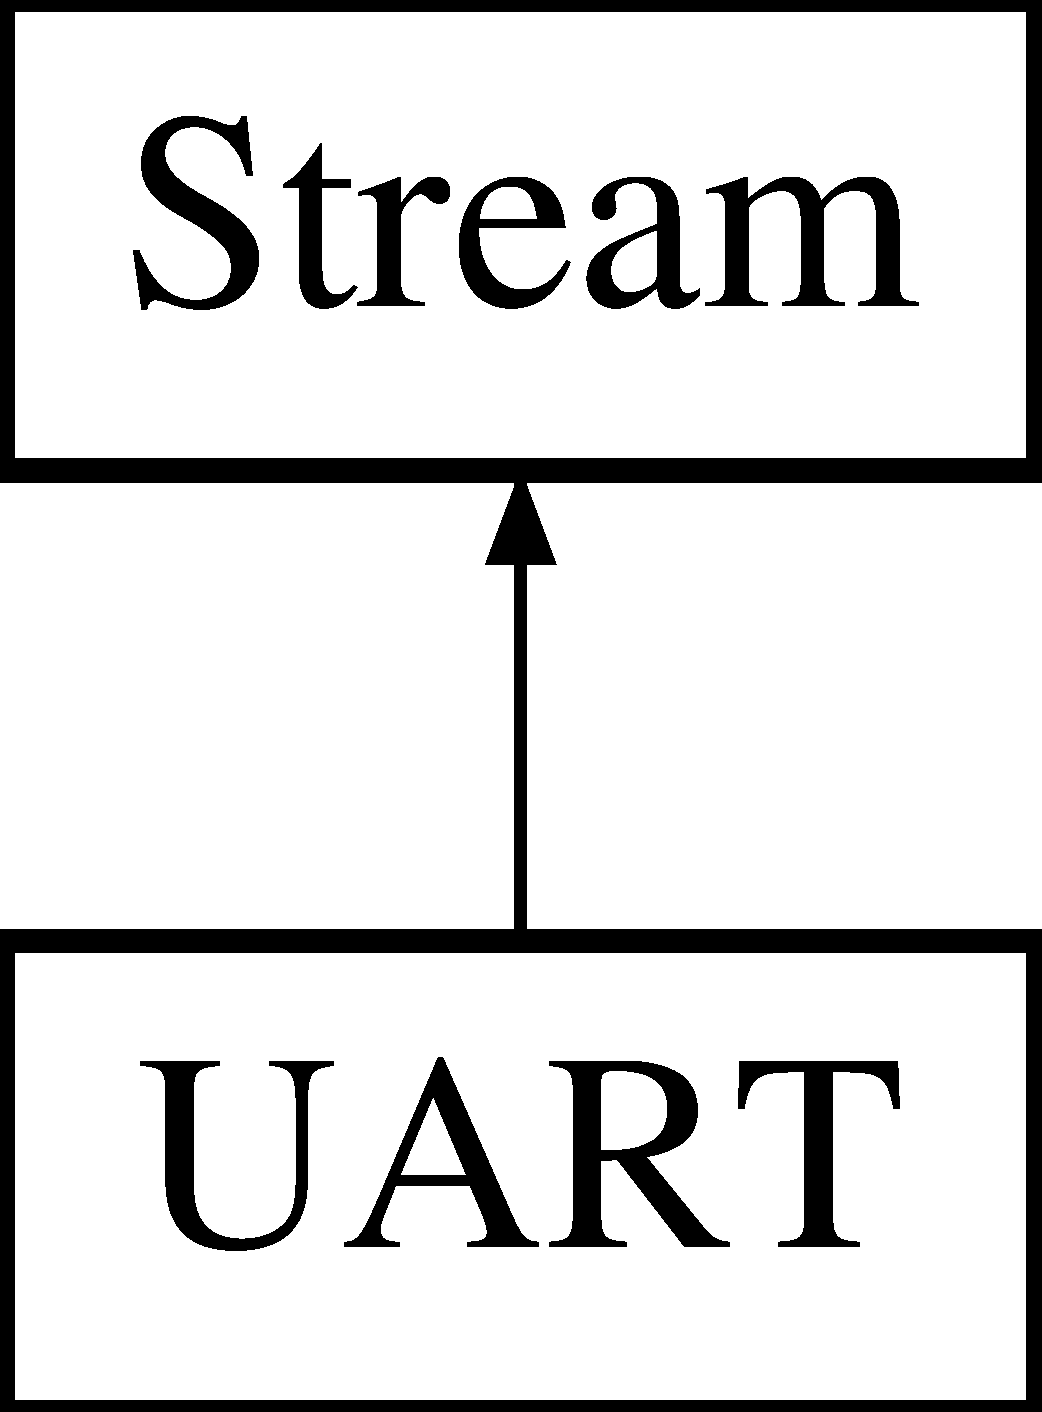
\includegraphics[height=2.000000cm]{class_u_a_r_t}
\end{center}
\end{figure}
\subsection*{Public Member Functions}
\begin{DoxyCompactItemize}
\item 
void \hyperlink{class_u_a_r_t_a8bb77ca27b4e17d608d2743313625ac4}{Write} (uint8\-\_\-t $\ast$string, uint16\-\_\-t size)
\item 
void \hyperlink{class_u_a_r_t_aed659ee8bc31ba966144d1a522506a7b}{Init} (uint16\-\_\-t baud\-\_\-rate)
\item 
\hyperlink{class_u_a_r_t_a97debffc29b178c09b104f4542298a36}{U\-A\-R\-T} (const \hyperlink{class_u_a_r_t}{U\-A\-R\-T} \&)=delete
\item 
void \hyperlink{class_u_a_r_t_a843ab7fc20f5ce5f030d2ca5ee98d6b6}{operator=} (const \hyperlink{class_u_a_r_t}{U\-A\-R\-T} \&)=delete
\end{DoxyCompactItemize}
\subsection*{Static Public Member Functions}
\begin{DoxyCompactItemize}
\item 
static \hyperlink{class_u_a_r_t}{U\-A\-R\-T} \& \hyperlink{class_u_a_r_t_a745c8f35f3ca3ab6359cedda3e640777}{Get\-Instance} ()
\end{DoxyCompactItemize}
\subsection*{Private Member Functions}
\begin{DoxyCompactItemize}
\item 
\hypertarget{class_u_a_r_t_a195cdcca08c2ae1d03ee8bf13a87b95a}{void {\bfseries initialize\-\_\-transmission} ()}\label{class_u_a_r_t_a195cdcca08c2ae1d03ee8bf13a87b95a}

\item 
\hyperlink{class_u_a_r_t_a68e7e88d2a13f5da85f0fde1ef98515f}{U\-A\-R\-T} ()
\end{DoxyCompactItemize}
\subsection*{Private Attributes}
\begin{DoxyCompactItemize}
\item 
\hypertarget{class_u_a_r_t_ae98e7d277a1833478aa85dc9e686150a}{bool {\bfseries ongoing\-\_\-transmission} = false}\label{class_u_a_r_t_ae98e7d277a1833478aa85dc9e686150a}

\end{DoxyCompactItemize}
\subsection*{Friends}
\begin{DoxyCompactItemize}
\item 
void \hyperlink{class_u_a_r_t_accc13d37cd82c841e387e1d5cf4d9a94}{U\-S\-A\-R\-T0\-\_\-\-U\-D\-R\-E\-\_\-vect} ()
\end{DoxyCompactItemize}
\subsection*{Additional Inherited Members}


\subsection{Constructor \& Destructor Documentation}
\hypertarget{class_u_a_r_t_a97debffc29b178c09b104f4542298a36}{\index{U\-A\-R\-T@{U\-A\-R\-T}!U\-A\-R\-T@{U\-A\-R\-T}}
\index{U\-A\-R\-T@{U\-A\-R\-T}!UART@{U\-A\-R\-T}}
\subsubsection[{U\-A\-R\-T}]{\setlength{\rightskip}{0pt plus 5cm}U\-A\-R\-T\-::\-U\-A\-R\-T (
\begin{DoxyParamCaption}
\item[{const {\bf U\-A\-R\-T} \&}]{}
\end{DoxyParamCaption}
)\hspace{0.3cm}{\ttfamily [delete]}}}\label{class_u_a_r_t_a97debffc29b178c09b104f4542298a36}
Beacause of singleton -\/ makes sure its not copied etc. \hypertarget{class_u_a_r_t_a68e7e88d2a13f5da85f0fde1ef98515f}{\index{U\-A\-R\-T@{U\-A\-R\-T}!U\-A\-R\-T@{U\-A\-R\-T}}
\index{U\-A\-R\-T@{U\-A\-R\-T}!UART@{U\-A\-R\-T}}
\subsubsection[{U\-A\-R\-T}]{\setlength{\rightskip}{0pt plus 5cm}U\-A\-R\-T\-::\-U\-A\-R\-T (
\begin{DoxyParamCaption}
{}
\end{DoxyParamCaption}
)\hspace{0.3cm}{\ttfamily [private]}}}\label{class_u_a_r_t_a68e7e88d2a13f5da85f0fde1ef98515f}
A constructor that initializes the \hyperlink{class_u_a_r_t}{U\-A\-R\-T} to a certain size 

\subsection{Member Function Documentation}
\hypertarget{class_u_a_r_t_a745c8f35f3ca3ab6359cedda3e640777}{\index{U\-A\-R\-T@{U\-A\-R\-T}!Get\-Instance@{Get\-Instance}}
\index{Get\-Instance@{Get\-Instance}!UART@{U\-A\-R\-T}}
\subsubsection[{Get\-Instance}]{\setlength{\rightskip}{0pt plus 5cm}static {\bf U\-A\-R\-T}\& U\-A\-R\-T\-::\-Get\-Instance (
\begin{DoxyParamCaption}
{}
\end{DoxyParamCaption}
)\hspace{0.3cm}{\ttfamily [inline]}, {\ttfamily [static]}}}\label{class_u_a_r_t_a745c8f35f3ca3ab6359cedda3e640777}
A Singleton implementation of this class \hypertarget{class_u_a_r_t_aed659ee8bc31ba966144d1a522506a7b}{\index{U\-A\-R\-T@{U\-A\-R\-T}!Init@{Init}}
\index{Init@{Init}!UART@{U\-A\-R\-T}}
\subsubsection[{Init}]{\setlength{\rightskip}{0pt plus 5cm}void U\-A\-R\-T\-::\-Init (
\begin{DoxyParamCaption}
\item[{uint16\-\_\-t}]{baud\-\_\-rate}
\end{DoxyParamCaption}
)}}\label{class_u_a_r_t_aed659ee8bc31ba966144d1a522506a7b}
Initializer because of the singleton implementation. 
\begin{DoxyParams}{Parameters}
{\em baud\-\_\-rate} & The baud rate of the uart \\
\hline
\end{DoxyParams}
\hypertarget{class_u_a_r_t_a843ab7fc20f5ce5f030d2ca5ee98d6b6}{\index{U\-A\-R\-T@{U\-A\-R\-T}!operator=@{operator=}}
\index{operator=@{operator=}!UART@{U\-A\-R\-T}}
\subsubsection[{operator=}]{\setlength{\rightskip}{0pt plus 5cm}void U\-A\-R\-T\-::operator= (
\begin{DoxyParamCaption}
\item[{const {\bf U\-A\-R\-T} \&}]{}
\end{DoxyParamCaption}
)\hspace{0.3cm}{\ttfamily [delete]}}}\label{class_u_a_r_t_a843ab7fc20f5ce5f030d2ca5ee98d6b6}
Beacause of singleton -\/ makes sure its not copied etc. \hypertarget{class_u_a_r_t_a8bb77ca27b4e17d608d2743313625ac4}{\index{U\-A\-R\-T@{U\-A\-R\-T}!Write@{Write}}
\index{Write@{Write}!UART@{U\-A\-R\-T}}
\subsubsection[{Write}]{\setlength{\rightskip}{0pt plus 5cm}void U\-A\-R\-T\-::\-Write (
\begin{DoxyParamCaption}
\item[{uint8\-\_\-t $\ast$}]{string, }
\item[{uint16\-\_\-t}]{size}
\end{DoxyParamCaption}
)\hspace{0.3cm}{\ttfamily [virtual]}}}\label{class_u_a_r_t_a8bb77ca27b4e17d608d2743313625ac4}
Write the inserted string to output (i.\-e. write to computer) 
\begin{DoxyParams}{Parameters}
{\em string} & The \char`\"{}data string\char`\"{} that shall be written to the output \\
\hline
{\em size} & the size of the data string \\
\hline
\end{DoxyParams}


Reimplemented from \hyperlink{class_stream_a508be3423e4d99ab2757275fb723002a}{Stream}.



\subsection{Friends And Related Function Documentation}
\hypertarget{class_u_a_r_t_accc13d37cd82c841e387e1d5cf4d9a94}{\index{U\-A\-R\-T@{U\-A\-R\-T}!U\-S\-A\-R\-T0\-\_\-\-U\-D\-R\-E\-\_\-vect@{U\-S\-A\-R\-T0\-\_\-\-U\-D\-R\-E\-\_\-vect}}
\index{U\-S\-A\-R\-T0\-\_\-\-U\-D\-R\-E\-\_\-vect@{U\-S\-A\-R\-T0\-\_\-\-U\-D\-R\-E\-\_\-vect}!UART@{U\-A\-R\-T}}
\subsubsection[{U\-S\-A\-R\-T0\-\_\-\-U\-D\-R\-E\-\_\-vect}]{\setlength{\rightskip}{0pt plus 5cm}void U\-S\-A\-R\-T0\-\_\-\-U\-D\-R\-E\-\_\-vect (
\begin{DoxyParamCaption}
{}
\end{DoxyParamCaption}
)\hspace{0.3cm}{\ttfamily [friend]}}}\label{class_u_a_r_t_accc13d37cd82c841e387e1d5cf4d9a94}
The interrupt handler vector. To be run on each D\-R\-E interrupt 

The documentation for this class was generated from the following files\-:\begin{DoxyCompactItemize}
\item 
lib/uart/\hyperlink{uart_8h}{uart.\-h}\item 
lib/uart/uart.\-cpp\end{DoxyCompactItemize}

\chapter{File Documentation}
\hypertarget{oled_8h}{\section{lib/oled/oled.h File Reference}
\label{oled_8h}\index{lib/oled/oled.\-h@{lib/oled/oled.\-h}}
}
{\ttfamily \#include \char`\"{}../stream/stream.\-h\char`\"{}}\\*
{\ttfamily \#include $<$avr/io.\-h$>$}\\*
\subsection*{Classes}
\begin{DoxyCompactItemize}
\item 
class \hyperlink{class_o_l_e_d}{O\-L\-E\-D}
\end{DoxyCompactItemize}


\subsection{Detailed Description}
\begin{DoxyAuthor}{Author}
Johan Lofstad, Sondre Baugstø and Sondre Russvoll 
\end{DoxyAuthor}
\begin{DoxyVersion}{Version}
1.\-0
\end{DoxyVersion}
An interface to communicate with the oled display 
\hypertarget{spi_8h}{}\section{lib/spi/spi.h File Reference}
\label{spi_8h}\index{lib/spi/spi.\+h@{lib/spi/spi.\+h}}
{\ttfamily \#include \char`\"{}../stream/stream.\+h\char`\"{}}\\*
{\ttfamily \#include $<$avr/io.\+h$>$}\\*
{\ttfamily \#include $<$avr/interrupt.\+h$>$}\\*
\subsection*{Classes}
\begin{DoxyCompactItemize}
\item 
struct \hyperlink{struct_s_p_i___n_1_1_p_i_n}{S\+P\+I\+\_\+\+N\+::\+P\+IN}
\item 
class \hyperlink{class_s_p_i___n_1_1_s_p_i}{S\+P\+I\+\_\+\+N\+::\+S\+PI}
\end{DoxyCompactItemize}
\subsection*{Functions}
\begin{DoxyCompactItemize}
\item 
{\bfseries S\+P\+I\+\_\+\+N\+::\+I\+SR} (S\+P\+I\+\_\+\+S\+T\+C\+\_\+vect)\hypertarget{spi_8h_af9dd63511a1eced9ad21190a5f10ea65}{}\label{spi_8h_af9dd63511a1eced9ad21190a5f10ea65}

\end{DoxyCompactItemize}


\subsection{Detailed Description}
\begin{DoxyAuthor}{Author}
Johan Lofstad, Sondre Baugstø, Sondre Russvoll 
\end{DoxyAuthor}
\begin{DoxyVersion}{Version}
1.\+0
\end{DoxyVersion}
An S\+PI driver 
\hypertarget{stream_8h}{\section{lib/stream/stream.h File Reference}
\label{stream_8h}\index{lib/stream/stream.\-h@{lib/stream/stream.\-h}}
}
{\ttfamily \#include $<$string.\-h$>$}\\*
{\ttfamily \#include $<$avr/io.\-h$>$}\\*
\subsection*{Classes}
\begin{DoxyCompactItemize}
\item 
class \hyperlink{class_stream}{Stream}
\end{DoxyCompactItemize}


\subsection{Detailed Description}
\begin{DoxyAuthor}{Author}
Johan Lofstad, Sondre Baugstø, Sondre Russvoll 
\end{DoxyAuthor}
\begin{DoxyVersion}{Version}
1.\-0
\end{DoxyVersion}
An interface for handling streams with default methods. 
\hypertarget{uart_8h}{}\section{lib/uart/uart.h File Reference}
\label{uart_8h}\index{lib/uart/uart.\+h@{lib/uart/uart.\+h}}
{\ttfamily \#include $<$avr/io.\+h$>$}\newline
{\ttfamily \#include $<$avr/interrupt.\+h$>$}\newline
{\ttfamily \#include \char`\"{}../stream/stream.\+h\char`\"{}}\newline
\subsection*{Classes}
\begin{DoxyCompactItemize}
\item 
class \hyperlink{class_u_a_r_t}{U\+A\+RT}
\end{DoxyCompactItemize}
\subsection*{Macros}
\begin{DoxyCompactItemize}
\item 
\hypertarget{uart_8h_a711e9130c825a7269c8c87dbb57a85e0}{}\label{uart_8h_a711e9130c825a7269c8c87dbb57a85e0} 
\#define {\bfseries M\+Y\+U\+B\+RR}~F\+O\+SC/16/B\+A\+UD-\/1
\end{DoxyCompactItemize}
\subsection*{Functions}
\begin{DoxyCompactItemize}
\item 
\hypertarget{uart_8h_a95e67e677722a53e3ad9f1ffce2e7408}{}\label{uart_8h_a95e67e677722a53e3ad9f1ffce2e7408} 
{\bfseries I\+SR} (U\+S\+A\+R\+T0\+\_\+\+U\+D\+R\+E\+\_\+vect)
\end{DoxyCompactItemize}


\subsection{Detailed Description}
\begin{DoxyAuthor}{Author}
Johan Lofstad, Sondre Baugstø and Sondre Russvoll 
\end{DoxyAuthor}
\begin{DoxyVersion}{Version}
1.\+1
\end{DoxyVersion}
An interface for communicating through \hyperlink{class_u_a_r_t}{U\+A\+RT} 
%--- End generated contents ---

% Index
\backmatter
\newpage
\phantomsection
\clearemptydoublepage
\addcontentsline{toc}{chapter}{Index}
\printindex

\end{document}
